% Options for packages loaded elsewhere
\PassOptionsToPackage{unicode}{hyperref}
\PassOptionsToPackage{hyphens}{url}
%
\documentclass[
]{book}
\usepackage{amsmath,amssymb}
\usepackage{iftex}
\ifPDFTeX
  \usepackage[T1]{fontenc}
  \usepackage[utf8]{inputenc}
  \usepackage{textcomp} % provide euro and other symbols
\else % if luatex or xetex
  \usepackage{unicode-math} % this also loads fontspec
  \defaultfontfeatures{Scale=MatchLowercase}
  \defaultfontfeatures[\rmfamily]{Ligatures=TeX,Scale=1}
\fi
\usepackage{lmodern}
\ifPDFTeX\else
  % xetex/luatex font selection
\fi
% Use upquote if available, for straight quotes in verbatim environments
\IfFileExists{upquote.sty}{\usepackage{upquote}}{}
\IfFileExists{microtype.sty}{% use microtype if available
  \usepackage[]{microtype}
  \UseMicrotypeSet[protrusion]{basicmath} % disable protrusion for tt fonts
}{}
\makeatletter
\@ifundefined{KOMAClassName}{% if non-KOMA class
  \IfFileExists{parskip.sty}{%
    \usepackage{parskip}
  }{% else
    \setlength{\parindent}{0pt}
    \setlength{\parskip}{6pt plus 2pt minus 1pt}}
}{% if KOMA class
  \KOMAoptions{parskip=half}}
\makeatother
\usepackage{xcolor}
\usepackage{color}
\usepackage{fancyvrb}
\newcommand{\VerbBar}{|}
\newcommand{\VERB}{\Verb[commandchars=\\\{\}]}
\DefineVerbatimEnvironment{Highlighting}{Verbatim}{commandchars=\\\{\}}
% Add ',fontsize=\small' for more characters per line
\usepackage{framed}
\definecolor{shadecolor}{RGB}{248,248,248}
\newenvironment{Shaded}{\begin{snugshade}}{\end{snugshade}}
\newcommand{\AlertTok}[1]{\textcolor[rgb]{0.94,0.16,0.16}{#1}}
\newcommand{\AnnotationTok}[1]{\textcolor[rgb]{0.56,0.35,0.01}{\textbf{\textit{#1}}}}
\newcommand{\AttributeTok}[1]{\textcolor[rgb]{0.13,0.29,0.53}{#1}}
\newcommand{\BaseNTok}[1]{\textcolor[rgb]{0.00,0.00,0.81}{#1}}
\newcommand{\BuiltInTok}[1]{#1}
\newcommand{\CharTok}[1]{\textcolor[rgb]{0.31,0.60,0.02}{#1}}
\newcommand{\CommentTok}[1]{\textcolor[rgb]{0.56,0.35,0.01}{\textit{#1}}}
\newcommand{\CommentVarTok}[1]{\textcolor[rgb]{0.56,0.35,0.01}{\textbf{\textit{#1}}}}
\newcommand{\ConstantTok}[1]{\textcolor[rgb]{0.56,0.35,0.01}{#1}}
\newcommand{\ControlFlowTok}[1]{\textcolor[rgb]{0.13,0.29,0.53}{\textbf{#1}}}
\newcommand{\DataTypeTok}[1]{\textcolor[rgb]{0.13,0.29,0.53}{#1}}
\newcommand{\DecValTok}[1]{\textcolor[rgb]{0.00,0.00,0.81}{#1}}
\newcommand{\DocumentationTok}[1]{\textcolor[rgb]{0.56,0.35,0.01}{\textbf{\textit{#1}}}}
\newcommand{\ErrorTok}[1]{\textcolor[rgb]{0.64,0.00,0.00}{\textbf{#1}}}
\newcommand{\ExtensionTok}[1]{#1}
\newcommand{\FloatTok}[1]{\textcolor[rgb]{0.00,0.00,0.81}{#1}}
\newcommand{\FunctionTok}[1]{\textcolor[rgb]{0.13,0.29,0.53}{\textbf{#1}}}
\newcommand{\ImportTok}[1]{#1}
\newcommand{\InformationTok}[1]{\textcolor[rgb]{0.56,0.35,0.01}{\textbf{\textit{#1}}}}
\newcommand{\KeywordTok}[1]{\textcolor[rgb]{0.13,0.29,0.53}{\textbf{#1}}}
\newcommand{\NormalTok}[1]{#1}
\newcommand{\OperatorTok}[1]{\textcolor[rgb]{0.81,0.36,0.00}{\textbf{#1}}}
\newcommand{\OtherTok}[1]{\textcolor[rgb]{0.56,0.35,0.01}{#1}}
\newcommand{\PreprocessorTok}[1]{\textcolor[rgb]{0.56,0.35,0.01}{\textit{#1}}}
\newcommand{\RegionMarkerTok}[1]{#1}
\newcommand{\SpecialCharTok}[1]{\textcolor[rgb]{0.81,0.36,0.00}{\textbf{#1}}}
\newcommand{\SpecialStringTok}[1]{\textcolor[rgb]{0.31,0.60,0.02}{#1}}
\newcommand{\StringTok}[1]{\textcolor[rgb]{0.31,0.60,0.02}{#1}}
\newcommand{\VariableTok}[1]{\textcolor[rgb]{0.00,0.00,0.00}{#1}}
\newcommand{\VerbatimStringTok}[1]{\textcolor[rgb]{0.31,0.60,0.02}{#1}}
\newcommand{\WarningTok}[1]{\textcolor[rgb]{0.56,0.35,0.01}{\textbf{\textit{#1}}}}
\usepackage{longtable,booktabs,array}
\usepackage{calc} % for calculating minipage widths
% Correct order of tables after \paragraph or \subparagraph
\usepackage{etoolbox}
\makeatletter
\patchcmd\longtable{\par}{\if@noskipsec\mbox{}\fi\par}{}{}
\makeatother
% Allow footnotes in longtable head/foot
\IfFileExists{footnotehyper.sty}{\usepackage{footnotehyper}}{\usepackage{footnote}}
\makesavenoteenv{longtable}
\usepackage{graphicx}
\makeatletter
\def\maxwidth{\ifdim\Gin@nat@width>\linewidth\linewidth\else\Gin@nat@width\fi}
\def\maxheight{\ifdim\Gin@nat@height>\textheight\textheight\else\Gin@nat@height\fi}
\makeatother
% Scale images if necessary, so that they will not overflow the page
% margins by default, and it is still possible to overwrite the defaults
% using explicit options in \includegraphics[width, height, ...]{}
\setkeys{Gin}{width=\maxwidth,height=\maxheight,keepaspectratio}
% Set default figure placement to htbp
\makeatletter
\def\fps@figure{htbp}
\makeatother
\setlength{\emergencystretch}{3em} % prevent overfull lines
\providecommand{\tightlist}{%
  \setlength{\itemsep}{0pt}\setlength{\parskip}{0pt}}
\setcounter{secnumdepth}{5}
\usepackage{booktabs}
\ifLuaTeX
  \usepackage{selnolig}  % disable illegal ligatures
\fi
\usepackage[]{natbib}
\bibliographystyle{plainnat}
\IfFileExists{bookmark.sty}{\usepackage{bookmark}}{\usepackage{hyperref}}
\IfFileExists{xurl.sty}{\usepackage{xurl}}{} % add URL line breaks if available
\urlstyle{same}
\hypersetup{
  pdftitle={A Minimal Book on R},
  pdfauthor={Pascal Bessonneau},
  hidelinks,
  pdfcreator={LaTeX via pandoc}}

\title{A Minimal Book on R}
\author{Pascal Bessonneau}
\date{2024-04-09}

\begin{document}
\maketitle

{
\setcounter{tocdepth}{1}
\tableofcontents
}
\hypertarget{objectif}{%
\chapter{Objectif}\label{objectif}}

Ce document constitue la trame du cours sur R pour les doctorants ``orientation''
du CRTD du CNAM.

Il n'est pas exhaustif et se place plutôt en appui du cours de M. Kilani. Il est
construit sur les bases et sur les difficultés du langage.

\hypertarget{architecture-de-r}{%
\chapter{Architecture de R}\label{architecture-de-r}}

R est à l'origine un logiciel de statistiques. Pour en faciliter l'usage il y
avait une interface très rugueuse qui était livré avec sous Windows.

Pour l'utiliser, en fait, il fallait écrire le code dans un bloc-notes (le code
est du texte brut) et le coller dans la console de R.

Vous pouvez toujours voir ce que ça donne en lançant R et non pas RStudio
sur votre bureau. En prenant la mesure qu'il y a eu beaucoup de progrès de fait.

Maintenant il existe RStudio, racheté par Posit. En fait c'est éditeur de texte
grandement amélioré.

Vous tapez le script dans la fenêtre en haut à gauche et vous l'exécutez en
cliquant sur l'icone ou CTRL+ENTREE. Vous pouvez limiter ce que vous exécutez
en sélectionnant du texte dans l'éditeur, seul le texte sélectionné sera soumis.

En clair, comme RStudio est un éditeur amélioré :
- le code qui n'est pas soumis, R ne le reconnait pas. Si vous créez une variable
en ligne 4 mais que vous ne le soumettez pas, quand vous aurez besoin de la
variable en ligne 30, elle n'existera pas.
- l'éditeur de texte peut contenir autre chose que du texte simple. Par exemple
du RMarkdown comme c'est le cas pour ce document. C'est un langage qui produit
de l'HTML c'est-à-dire des pages web. Le Markdown est très simple, le langage
tient sur une feuille : \href{https://www.markdownguide.org/cheat-sheet/}{ici}.
- ou du LaTeX avec le mode knitr
- On peut des graphiques R dans la fenêtre RStudio (en bas à droite)
- RStudio peut servir pour la gestion de paquets
- \ldots{}

RStudio fait donc beaucoup de choses.

A noter que Jamovi et JASP utilisent aussi R sauf que pour eux ce n'est presque
plus visible. A part dans les extensions et/ou les modules. Il y a des modules
Jamovi pour écrire du code R ou pour faire des modèles structuraux directement
en R dans Jamovi.

Vous allez avoir une démonstration enregistré pour l'utilisation de RStudio.

Les autres choses à rappeler, c'est que R est un langage cassee dépendant :
- les noms de fonctions de R sont à écrire en \textbf{minuscules}
- un objet n'est pas le même si une ou plusieurs lettres sont en majuscule au lieu
d'être en minuscule.

\begin{Shaded}
\begin{Highlighting}[]
\NormalTok{aAa }\OtherTok{\textless{}{-}} \DecValTok{2}
\NormalTok{AAa }\OtherTok{\textless{}{-}} \DecValTok{4}
\end{Highlighting}
\end{Shaded}

donc

\begin{Shaded}
\begin{Highlighting}[]
\NormalTok{AAa}
\end{Highlighting}
\end{Shaded}

\begin{verbatim}
## [1] 4
\end{verbatim}

et

\begin{Shaded}
\begin{Highlighting}[]
\NormalTok{aAa}
\end{Highlighting}
\end{Shaded}

\begin{verbatim}
## [1] 2
\end{verbatim}

Les commentaires dans R sont à noter avec des \#. Tout ce qui suit le \# est un
commentaire.

Comme RStudio vous l'aurez remarqué vous aide en analysant et en colorant le
code, n'utilisez pas un script R pour mettre des remarques (et non du code) en
dehors de commentaires. Sinon c'est la catastrophe\ldots{}

\textbf{Utiliser toujours RStudio en mode Projet}

\hypertarget{paquets}{%
\section{Paquets}\label{paquets}}

Les fonctionnalités de R sont finalement assez limitées. Il fait un certain
nombre de statistiques et surtout fourni des outils mathématiques puissants
mais ça grande force est de proposer des paquets qui ajoute des fonctionnalités.

Ces paquets sont développés par des gens (qui font ça sur leur temps personnel
ou professionnel), des entreprises, des fondations, \ldots{}

La liste des paquets officiels est \href{https://cran.r-project.org/web/packages/available_packages_by_name.html}{là}

Ils sont maintenant pléthoriques et je vous conseille de vous reportez \href{https://cran.r-project.org/web/views/}{à cette page}.

Elles répertorient les paquets utiles par domaine d'application. De plus les
paquets un peu douteux en qualité n'y figure pas. Donc c'est du solide.

Pour cela je vous recommande de l'utiliser pour se faire, suivez les instructions ci-dessous:

\begin{Shaded}
\begin{Highlighting}[]
\FunctionTok{install.packages}\NormalTok{(}\StringTok{"ctv"}\NormalTok{)}
\end{Highlighting}
\end{Shaded}

Puis quand vous voulez installer une vue (SocialSciences par exemple) :

\begin{Shaded}
\begin{Highlighting}[]
\FunctionTok{library}\NormalTok{(ctv)}
\FunctionTok{install.views}\NormalTok{(}\StringTok{"SocialSciences"}\NormalTok{)}
\end{Highlighting}
\end{Shaded}

On vient de voir comment appeler un paquet :

\begin{Shaded}
\begin{Highlighting}[]
\FunctionTok{library}\NormalTok{(tidyverse)}
\end{Highlighting}
\end{Shaded}

ou

\begin{Shaded}
\begin{Highlighting}[]
\FunctionTok{require}\NormalTok{(tidyverse)}
\end{Highlighting}
\end{Shaded}

Cela revient presque au même. Presque. Pour commencer vous pouvez utiliser
\textbf{library} en priorité.

Essayez d'installer un paquet :

\begin{Shaded}
\begin{Highlighting}[]
\FunctionTok{install.packages}\NormalTok{(}\StringTok{"readxl"}\NormalTok{)}
\end{Highlighting}
\end{Shaded}

Maintenant vous pouvez lire les fichiers Excel. Vous n'avez besoin d'installer
le paquet qu'une fois mais vous devez le réclamer avec \textbf{library} la première
fois que vous l'utilisez dans un script. La politique est de charger tous les
paquets que vous utilisez \textbf{en tête du script}.

Maintenant on va faire des statistiques.

\hypertarget{le-langage-r}{%
\chapter{Le langage R}\label{le-langage-r}}

\hypertarget{introduction}{%
\section{Introduction}\label{introduction}}

Le but est d'aborder des notions et de voir quelques exemples.

R ne fonctionne pas comme JASP, Jamovi, SAS ou SPSS. Par exemple SPSS, vous ouvrez une
source de données et vous voyez vos données sur un tableur.

Quand vous passez une commande sur SPSS, il n'y a pas d'ambiguité, le traitement
se fait sur le tableur actif.

Avec SAS, on ajoute une dose de complexité, car vous avez des bibliothèques
et des tables.

Dans les deux cas, quand vous lancez une procédure statistique vous récupérez
les résultats dans une fenêtre dédié car il y a une séparation des données
et des résultats (dans la quasi-totalité des cas).

Avec R, c'est différent. R est un langage de programmation comme Python, Pascal,
Rust, etc.

La force de R et ce qui le rend compliqué est qu'il n'y a pas de séparation aussi
stricte entre données et résultats.

Vous avez des objets en mémoire dans R et ces objets peuvent servir aussi bien
de sources de données, d'arguments pour sélectionner une partie des résultats ou
bien être des résultats d'une opérations statistiques.

\hypertarget{un-exemple-de-traitement-de-donnuxe9es}{%
\section{Un exemple de traitement de données}\label{un-exemple-de-traitement-de-donnuxe9es}}

On va travailler sur une base de données qui sont les iris de Fisher. C'est
plus simple car c'est un jeu de données qui est en mémoire dans R, on verra
comment charger une source de données plus tard.

\begin{Shaded}
\begin{Highlighting}[]
\FunctionTok{data}\NormalTok{(iris)}
\end{Highlighting}
\end{Shaded}

Vous pouvez cliquer sur \textbf{iris} qui est apparu dans la fenêtre en haut
à droite de RStudio. Elle ouvre un tableur assez frustre mais qui permet
de visualiser les données.

Mais c'est une très mauvaise habitude d'utiliser ce tableur pour visualiser
les données.

Il vaut mieux taper :

\begin{Shaded}
\begin{Highlighting}[]
\FunctionTok{str}\NormalTok{(iris)}
\end{Highlighting}
\end{Shaded}

\begin{verbatim}
## 'data.frame':    150 obs. of  5 variables:
##  $ Sepal.Length: num  5.1 4.9 4.7 4.6 5 5.4 4.6 5 4.4 4.9 ...
##  $ Sepal.Width : num  3.5 3 3.2 3.1 3.6 3.9 3.4 3.4 2.9 3.1 ...
##  $ Petal.Length: num  1.4 1.4 1.3 1.5 1.4 1.7 1.4 1.5 1.4 1.5 ...
##  $ Petal.Width : num  0.2 0.2 0.2 0.2 0.2 0.4 0.3 0.2 0.2 0.1 ...
##  $ Species     : Factor w/ 3 levels "setosa","versicolor",..: 1 1 1 1 1 1 1 1 1 1 ...
\end{verbatim}

\textbf{str} c'est pour \textbf{structure}. Enfin je crois. Elle vous décrit quelle est la
nature de l'objet et de quoi il est composé. Ca peut être rudemment complexe.

Mais là non. Il nous dit que c'est une \textbf{data.frame}. Le type \textbf{data.frame}
est ce qui se rapproche le plus d'un tableau de données comme dans SPSS ou Jamovi.

R nous dit que la data.frame a 150 observations et 5 variables. La structure est
tabulaire comme dans Jamovi ou JASP: on a 150 relevés de plante (individus) et
on a gardé 5 éléments caractérisant l'individu.

\begin{itemize}
\tightlist
\item
  Sepal.Length : \textbf{num} veut dire \textbf{numeric}, c'est une taille de Sépale.
\item
  Sepal.Width : \textbf{num} veut dire \textbf{numeric}, c'est une taille de Sépale.
\item
  \ldots{}
\item
  Species : c'est l'espèce, qui peut prendre 3 valeurs. Dans un type appelé
  \textbf{Factor}
\end{itemize}

On voit que R sépare bien chacune des variables. Pour schématiser dans notre cas
nous avons des individus en ligne et des observations en colonne. Comme Jamovi.

\hypertarget{vecteurs}{%
\section{Vecteurs}\label{vecteurs}}

\hypertarget{exemple-de-vecteurs}{%
\subsection{Exemple de vecteurs}\label{exemple-de-vecteurs}}

Là où ça devient différent c'est que la \textbf{data.frame} est en fait un aggrégat
d'élements plus simples.

Vous pouvez extraire par exemple la longueur des sépales pour tous les individus:

\begin{Shaded}
\begin{Highlighting}[]
\NormalTok{iris[,}\StringTok{"Sepal.Length"}\NormalTok{]}
\end{Highlighting}
\end{Shaded}

\begin{verbatim}
##   [1] 5.1 4.9 4.7 4.6 5.0 5.4 4.6 5.0 4.4 4.9 5.4 4.8 4.8 4.3 5.8 5.7 5.4 5.1 5.7 5.1 5.4 5.1 4.6 5.1 4.8 5.0 5.0 5.2 5.2
##  [30] 4.7 4.8 5.4 5.2 5.5 4.9 5.0 5.5 4.9 4.4 5.1 5.0 4.5 4.4 5.0 5.1 4.8 5.1 4.6 5.3 5.0 7.0 6.4 6.9 5.5 6.5 5.7 6.3 4.9
##  [59] 6.6 5.2 5.0 5.9 6.0 6.1 5.6 6.7 5.6 5.8 6.2 5.6 5.9 6.1 6.3 6.1 6.4 6.6 6.8 6.7 6.0 5.7 5.5 5.5 5.8 6.0 5.4 6.0 6.7
##  [88] 6.3 5.6 5.5 5.5 6.1 5.8 5.0 5.6 5.7 5.7 6.2 5.1 5.7 6.3 5.8 7.1 6.3 6.5 7.6 4.9 7.3 6.7 7.2 6.5 6.4 6.8 5.7 5.8 6.4
## [117] 6.5 7.7 7.7 6.0 6.9 5.6 7.7 6.3 6.7 7.2 6.2 6.1 6.4 7.2 7.4 7.9 6.4 6.3 6.1 7.7 6.3 6.4 6.0 6.9 6.7 6.9 5.8 6.8 6.7
## [146] 6.7 6.3 6.5 6.2 5.9
\end{verbatim}

Vous regardez par colonne, vous obtenez les valeurs pour les 150 individus.

Si vous regardez la structure de ce que vous avez obtenu :

\begin{Shaded}
\begin{Highlighting}[]
\FunctionTok{str}\NormalTok{(iris[,}\StringTok{"Sepal.Length"}\NormalTok{])}
\end{Highlighting}
\end{Shaded}

\begin{verbatim}
##  num [1:150] 5.1 4.9 4.7 4.6 5 5.4 4.6 5 4.4 4.9 ...
\end{verbatim}

Vous voyez que ce qui s'affichait tout à l'heure sur la \textbf{data.frame}.

Vous pouvez calculer la moyenne des longueurs:

\begin{Shaded}
\begin{Highlighting}[]
\FunctionTok{mean}\NormalTok{(iris[,}\StringTok{"Sepal.Length"}\NormalTok{])}
\end{Highlighting}
\end{Shaded}

\begin{verbatim}
## [1] 5.843333
\end{verbatim}

Vous venez de faire une opération sur un vecteur. C'est un ensemble qui est typé
ici des numériques mais ça peut être du texte, des entiers, etc. respectivement
\textbf{character}, \textbf{integer}, etc.

Vous pouvez extraire ce vecteur :

\begin{Shaded}
\begin{Highlighting}[]
\NormalTok{longueur.sepale }\OtherTok{\textless{}{-}}\NormalTok{ iris[,}\StringTok{"Sepal.Length"}\NormalTok{]}
\end{Highlighting}
\end{Shaded}

Vous remarquez que R n'affiche pas le résultat de l'opération car on ne lui demande
pas de résultat. On affecte la partie à droite de ``\textless-'' à la partie gauche.

Si on fait:

\begin{Shaded}
\begin{Highlighting}[]
\NormalTok{longueur.sepale}
\end{Highlighting}
\end{Shaded}

\begin{verbatim}
##   [1] 5.1 4.9 4.7 4.6 5.0 5.4 4.6 5.0 4.4 4.9 5.4 4.8 4.8 4.3 5.8 5.7 5.4 5.1 5.7 5.1 5.4 5.1 4.6 5.1 4.8 5.0 5.0 5.2 5.2
##  [30] 4.7 4.8 5.4 5.2 5.5 4.9 5.0 5.5 4.9 4.4 5.1 5.0 4.5 4.4 5.0 5.1 4.8 5.1 4.6 5.3 5.0 7.0 6.4 6.9 5.5 6.5 5.7 6.3 4.9
##  [59] 6.6 5.2 5.0 5.9 6.0 6.1 5.6 6.7 5.6 5.8 6.2 5.6 5.9 6.1 6.3 6.1 6.4 6.6 6.8 6.7 6.0 5.7 5.5 5.5 5.8 6.0 5.4 6.0 6.7
##  [88] 6.3 5.6 5.5 5.5 6.1 5.8 5.0 5.6 5.7 5.7 6.2 5.1 5.7 6.3 5.8 7.1 6.3 6.5 7.6 4.9 7.3 6.7 7.2 6.5 6.4 6.8 5.7 5.8 6.4
## [117] 6.5 7.7 7.7 6.0 6.9 5.6 7.7 6.3 6.7 7.2 6.2 6.1 6.4 7.2 7.4 7.9 6.4 6.3 6.1 7.7 6.3 6.4 6.0 6.9 6.7 6.9 5.8 6.8 6.7
## [146] 6.7 6.3 6.5 6.2 5.9
\end{verbatim}

On retrouve bien nos longueurs.

On peut en calculer la moyenne :

\begin{Shaded}
\begin{Highlighting}[]
\FunctionTok{mean}\NormalTok{(longueur.sepale)}
\end{Highlighting}
\end{Shaded}

\begin{verbatim}
## [1] 5.843333
\end{verbatim}

Qu'est ce qui se passe ? En fait on a indexé notre \textbf{data.frame}.

On a dit à R, renvoie nous la variable ``Sepal.Length'' et nous avons décidé de le
stocker dans une variable autre.

\hypertarget{cruxe9ation-de-vecteurs}{%
\subsection{Création de vecteurs}\label{cruxe9ation-de-vecteurs}}

Pour créer un vecteur, il faut utiliser la fonction \textbf{c} pour \textbf{concatenate}.

Exemple :

\begin{Shaded}
\begin{Highlighting}[]
\FunctionTok{c}\NormalTok{(}\StringTok{"Sepal.Length"}\NormalTok{,}\StringTok{"Petal.Length"}\NormalTok{)}
\end{Highlighting}
\end{Shaded}

\begin{verbatim}
## [1] "Sepal.Length" "Petal.Length"
\end{verbatim}

On peut l'affecter à une variable:

\begin{Shaded}
\begin{Highlighting}[]
\NormalTok{longueurs }\OtherTok{\textless{}{-}} \FunctionTok{c}\NormalTok{(}\StringTok{"Sepal.Length"}\NormalTok{,}\StringTok{"Petal.Length"}\NormalTok{)}
\end{Highlighting}
\end{Shaded}

C'est un vecteur :

\begin{Shaded}
\begin{Highlighting}[]
\FunctionTok{str}\NormalTok{(longueurs)}
\end{Highlighting}
\end{Shaded}

\begin{verbatim}
##  chr [1:2] "Sepal.Length" "Petal.Length"
\end{verbatim}

Maintenant on peut faire:

\begin{Shaded}
\begin{Highlighting}[]
\NormalTok{iris[,longueurs]}
\end{Highlighting}
\end{Shaded}

\begin{verbatim}
##     Sepal.Length Petal.Length
## 1            5.1          1.4
## 2            4.9          1.4
## 3            4.7          1.3
## 4            4.6          1.5
## 5            5.0          1.4
## 6            5.4          1.7
## 7            4.6          1.4
## 8            5.0          1.5
## 9            4.4          1.4
## 10           4.9          1.5
## 11           5.4          1.5
## 12           4.8          1.6
## 13           4.8          1.4
## 14           4.3          1.1
## 15           5.8          1.2
## 16           5.7          1.5
## 17           5.4          1.3
## 18           5.1          1.4
## 19           5.7          1.7
## 20           5.1          1.5
## 21           5.4          1.7
## 22           5.1          1.5
## 23           4.6          1.0
## 24           5.1          1.7
## 25           4.8          1.9
## 26           5.0          1.6
## 27           5.0          1.6
## 28           5.2          1.5
## 29           5.2          1.4
## 30           4.7          1.6
## 31           4.8          1.6
## 32           5.4          1.5
## 33           5.2          1.5
## 34           5.5          1.4
## 35           4.9          1.5
## 36           5.0          1.2
## 37           5.5          1.3
## 38           4.9          1.4
## 39           4.4          1.3
## 40           5.1          1.5
## 41           5.0          1.3
## 42           4.5          1.3
## 43           4.4          1.3
## 44           5.0          1.6
## 45           5.1          1.9
## 46           4.8          1.4
## 47           5.1          1.6
## 48           4.6          1.4
## 49           5.3          1.5
## 50           5.0          1.4
## 51           7.0          4.7
## 52           6.4          4.5
## 53           6.9          4.9
## 54           5.5          4.0
## 55           6.5          4.6
## 56           5.7          4.5
## 57           6.3          4.7
## 58           4.9          3.3
## 59           6.6          4.6
## 60           5.2          3.9
## 61           5.0          3.5
## 62           5.9          4.2
## 63           6.0          4.0
## 64           6.1          4.7
## 65           5.6          3.6
## 66           6.7          4.4
## 67           5.6          4.5
## 68           5.8          4.1
## 69           6.2          4.5
## 70           5.6          3.9
## 71           5.9          4.8
## 72           6.1          4.0
## 73           6.3          4.9
## 74           6.1          4.7
## 75           6.4          4.3
## 76           6.6          4.4
## 77           6.8          4.8
## 78           6.7          5.0
## 79           6.0          4.5
## 80           5.7          3.5
## 81           5.5          3.8
## 82           5.5          3.7
## 83           5.8          3.9
## 84           6.0          5.1
## 85           5.4          4.5
## 86           6.0          4.5
## 87           6.7          4.7
## 88           6.3          4.4
## 89           5.6          4.1
## 90           5.5          4.0
## 91           5.5          4.4
## 92           6.1          4.6
## 93           5.8          4.0
## 94           5.0          3.3
## 95           5.6          4.2
## 96           5.7          4.2
## 97           5.7          4.2
## 98           6.2          4.3
## 99           5.1          3.0
## 100          5.7          4.1
## 101          6.3          6.0
## 102          5.8          5.1
## 103          7.1          5.9
## 104          6.3          5.6
## 105          6.5          5.8
## 106          7.6          6.6
## 107          4.9          4.5
## 108          7.3          6.3
## 109          6.7          5.8
## 110          7.2          6.1
## 111          6.5          5.1
## 112          6.4          5.3
## 113          6.8          5.5
## 114          5.7          5.0
## 115          5.8          5.1
## 116          6.4          5.3
## 117          6.5          5.5
## 118          7.7          6.7
## 119          7.7          6.9
## 120          6.0          5.0
## 121          6.9          5.7
## 122          5.6          4.9
## 123          7.7          6.7
## 124          6.3          4.9
## 125          6.7          5.7
## 126          7.2          6.0
## 127          6.2          4.8
## 128          6.1          4.9
## 129          6.4          5.6
## 130          7.2          5.8
## 131          7.4          6.1
## 132          7.9          6.4
## 133          6.4          5.6
## 134          6.3          5.1
## 135          6.1          5.6
## 136          7.7          6.1
## 137          6.3          5.6
## 138          6.4          5.5
## 139          6.0          4.8
## 140          6.9          5.4
## 141          6.7          5.6
## 142          6.9          5.1
## 143          5.8          5.1
## 144          6.8          5.9
## 145          6.7          5.7
## 146          6.7          5.2
## 147          6.3          5.0
## 148          6.5          5.2
## 149          6.2          5.4
## 150          5.9          5.1
\end{verbatim}

On vient d'indexer iris avec un vecteur composé de deux noms qui sont les noms
des variables.

R lit la partie droite de la virgule et comprends que nous voulons les deux variables.
Quelle est la structure de ce que l'on récupère :

\begin{Shaded}
\begin{Highlighting}[]
\FunctionTok{str}\NormalTok{(iris[,longueurs])}
\end{Highlighting}
\end{Shaded}

\begin{verbatim}
## 'data.frame':    150 obs. of  2 variables:
##  $ Sepal.Length: num  5.1 4.9 4.7 4.6 5 5.4 4.6 5 4.4 4.9 ...
##  $ Petal.Length: num  1.4 1.4 1.3 1.5 1.4 1.7 1.4 1.5 1.4 1.5 ...
\end{verbatim}

C'est une \textbf{data.frame} les informations sur nos 150 individus pour les longueurs.

on peut faire:

\begin{Shaded}
\begin{Highlighting}[]
\NormalTok{iris.longueurs }\OtherTok{\textless{}{-}}\NormalTok{ iris[,longueurs]}
\FunctionTok{str}\NormalTok{(iris.longueurs)}
\end{Highlighting}
\end{Shaded}

\begin{verbatim}
## 'data.frame':    150 obs. of  2 variables:
##  $ Sepal.Length: num  5.1 4.9 4.7 4.6 5 5.4 4.6 5 4.4 4.9 ...
##  $ Petal.Length: num  1.4 1.4 1.3 1.5 1.4 1.7 1.4 1.5 1.4 1.5 ...
\end{verbatim}

\begin{Shaded}
\begin{Highlighting}[]
\NormalTok{iris.longueurs[,}\StringTok{"Sepal.Length"}\NormalTok{]}
\end{Highlighting}
\end{Shaded}

\begin{verbatim}
##   [1] 5.1 4.9 4.7 4.6 5.0 5.4 4.6 5.0 4.4 4.9 5.4 4.8 4.8 4.3 5.8 5.7 5.4 5.1 5.7 5.1 5.4 5.1 4.6 5.1 4.8 5.0 5.0 5.2 5.2
##  [30] 4.7 4.8 5.4 5.2 5.5 4.9 5.0 5.5 4.9 4.4 5.1 5.0 4.5 4.4 5.0 5.1 4.8 5.1 4.6 5.3 5.0 7.0 6.4 6.9 5.5 6.5 5.7 6.3 4.9
##  [59] 6.6 5.2 5.0 5.9 6.0 6.1 5.6 6.7 5.6 5.8 6.2 5.6 5.9 6.1 6.3 6.1 6.4 6.6 6.8 6.7 6.0 5.7 5.5 5.5 5.8 6.0 5.4 6.0 6.7
##  [88] 6.3 5.6 5.5 5.5 6.1 5.8 5.0 5.6 5.7 5.7 6.2 5.1 5.7 6.3 5.8 7.1 6.3 6.5 7.6 4.9 7.3 6.7 7.2 6.5 6.4 6.8 5.7 5.8 6.4
## [117] 6.5 7.7 7.7 6.0 6.9 5.6 7.7 6.3 6.7 7.2 6.2 6.1 6.4 7.2 7.4 7.9 6.4 6.3 6.1 7.7 6.3 6.4 6.0 6.9 6.7 6.9 5.8 6.8 6.7
## [146] 6.7 6.3 6.5 6.2 5.9
\end{verbatim}

\begin{Shaded}
\begin{Highlighting}[]
\FunctionTok{mean}\NormalTok{(iris.longueurs[,}\StringTok{"Sepal.Length"}\NormalTok{])}
\end{Highlighting}
\end{Shaded}

\begin{verbatim}
## [1] 5.843333
\end{verbatim}

\hypertarget{les-types-de-vecteurs}{%
\subsection{Les types de vecteurs}\label{les-types-de-vecteurs}}

les vecteurs en résumé peuvent être :
- des numéros entiers, \textbf{int}
- des chaines de caractères, \textbf{chr}
- des logiques, \textbf{logi}
- des réels, \textbf{num}
- \ldots{}

On peut créer un vecteur d'entiers

\begin{Shaded}
\begin{Highlighting}[]
\FunctionTok{c}\NormalTok{(}\DecValTok{1}\NormalTok{,}\DecValTok{3}\NormalTok{)}
\end{Highlighting}
\end{Shaded}

\begin{verbatim}
## [1] 1 3
\end{verbatim}

Un vecteur de logique: (T pour vrai, F pour faux)

\begin{Shaded}
\begin{Highlighting}[]
\FunctionTok{c}\NormalTok{(T,F,T,F,F)}
\end{Highlighting}
\end{Shaded}

\begin{verbatim}
## [1]  TRUE FALSE  TRUE FALSE FALSE
\end{verbatim}

Et là surprise : si on demande à R de nous retourner la première et la troisième
variable de iris

\begin{Shaded}
\begin{Highlighting}[]
\FunctionTok{str}\NormalTok{(iris[,}\FunctionTok{c}\NormalTok{(}\DecValTok{1}\NormalTok{,}\DecValTok{3}\NormalTok{)])}
\end{Highlighting}
\end{Shaded}

\begin{verbatim}
## 'data.frame':    150 obs. of  2 variables:
##  $ Sepal.Length: num  5.1 4.9 4.7 4.6 5 5.4 4.6 5 4.4 4.9 ...
##  $ Petal.Length: num  1.4 1.4 1.3 1.5 1.4 1.7 1.4 1.5 1.4 1.5 ...
\end{verbatim}

Plus compliqué. On sait qu'il y a 5 variables dans iris ? On est d'accord ?
Donc si on lui demande de nous renvoyer la variable quand c'est vrai et de ne pas
nous la renvoyer quand c'est faux ?

\begin{Shaded}
\begin{Highlighting}[]
\FunctionTok{str}\NormalTok{(iris[,}\FunctionTok{c}\NormalTok{(T,F,T,F,F)])}
\end{Highlighting}
\end{Shaded}

\begin{verbatim}
## 'data.frame':    150 obs. of  2 variables:
##  $ Sepal.Length: num  5.1 4.9 4.7 4.6 5 5.4 4.6 5 4.4 4.9 ...
##  $ Petal.Length: num  1.4 1.4 1.3 1.5 1.4 1.7 1.4 1.5 1.4 1.5 ...
\end{verbatim}

En fait les \textbf{data.frame}s sont des agrégats de vecteurs que l'on peut indexer
avec des vecteurs.

Pourquoi on ne peut pas faire :

\begin{Shaded}
\begin{Highlighting}[]
\FunctionTok{mean}\NormalTok{(iris.longueurs)}
\end{Highlighting}
\end{Shaded}

parce qu'on a deux variables ? R refuse de faire ce qui n'a pas de sens.

Après tout on voudrait faire la moyenne de sépale et de pétale. Déjà mais
ça pourrait être pire :

\begin{Shaded}
\begin{Highlighting}[]
\FunctionTok{mean}\NormalTok{(iris[,}\FunctionTok{c}\NormalTok{(}\StringTok{"Sepal.Length"}\NormalTok{,}\StringTok{"Species"}\NormalTok{)])}
\end{Highlighting}
\end{Shaded}

C'est la catastrophe. Vous essayez de faire une moyenne sur une variable texte
et une variable continue. C'est faux.

Pour faire le résumer d'une variable texte:

\begin{Shaded}
\begin{Highlighting}[]
\FunctionTok{table}\NormalTok{(iris[,}\StringTok{"Species"}\NormalTok{])}
\end{Highlighting}
\end{Shaded}

\begin{verbatim}
## 
##     setosa versicolor  virginica 
##         50         50         50
\end{verbatim}

\hypertarget{pour-ruxe9sumuxe9}{%
\subsection{Pour résumé}\label{pour-ruxe9sumuxe9}}

On a les \textbf{data.frame}, on a les \textbf{vector} de différents types. On sait qu'on
peut sélectionner les variables par l'intermédiaire de vecteurs.

\hypertarget{suxe9lection-des-individus}{%
\section{Sélection des individus}\label{suxe9lection-des-individus}}

Intuitivement, comment sélectionner des individus ?

Ca marche comme pour les variables, on utilise des vecteurs ?

On veut les individus de 1 et 5.

\begin{Shaded}
\begin{Highlighting}[]
\FunctionTok{str}\NormalTok{(iris[}\FunctionTok{c}\NormalTok{(}\DecValTok{1}\NormalTok{,}\DecValTok{5}\NormalTok{),])}
\end{Highlighting}
\end{Shaded}

\begin{verbatim}
## 'data.frame':    2 obs. of  5 variables:
##  $ Sepal.Length: num  5.1 5
##  $ Sepal.Width : num  3.5 3.6
##  $ Petal.Length: num  1.4 1.4
##  $ Petal.Width : num  0.2 0.2
##  $ Species     : Factor w/ 3 levels "setosa","versicolor",..: 1 1
\end{verbatim}

Attention à la place de la virgule. Cette fois on sélectionne des lignes. A gauche
de la virgule pour des lignes et à droite pour les colonnes.

C'est tout bon.

On a vu qu'il y avait trois espèces. Si on veut sélectionner ceux qui sont du type
\textbf{versicolor} ?

On se rappele des vecteurs de logique: là où iris{[},``Species''{]} vaudra \textbf{versicolor}
on sélectionne et là où ce n'est pas \textbf{versicolor} on ne sélectionne pas.

On ne va pas le faire à la main. On ne fait rien à la main sous R.

\begin{Shaded}
\begin{Highlighting}[]
\NormalTok{especes }\OtherTok{\textless{}{-}} \FunctionTok{c}\NormalTok{(}\StringTok{"versicolor"}\NormalTok{,}\StringTok{"truc"}\NormalTok{,}\StringTok{"versicolor"}\NormalTok{,}\StringTok{"setosa"}\NormalTok{)}
\NormalTok{especes}
\end{Highlighting}
\end{Shaded}

\begin{verbatim}
## [1] "versicolor" "truc"       "versicolor" "setosa"
\end{verbatim}

\begin{Shaded}
\begin{Highlighting}[]
\NormalTok{especes}\SpecialCharTok{==}\StringTok{"versicolor"}
\end{Highlighting}
\end{Shaded}

\begin{verbatim}
## [1]  TRUE FALSE  TRUE FALSE
\end{verbatim}

On l'adapte pour notre cas :

\begin{Shaded}
\begin{Highlighting}[]
\NormalTok{iris[,}\StringTok{"Species"}\NormalTok{]}\SpecialCharTok{==}\StringTok{"versicolor"}
\end{Highlighting}
\end{Shaded}

\begin{verbatim}
##   [1] FALSE FALSE FALSE FALSE FALSE FALSE FALSE FALSE FALSE FALSE FALSE FALSE FALSE FALSE FALSE FALSE FALSE FALSE FALSE
##  [20] FALSE FALSE FALSE FALSE FALSE FALSE FALSE FALSE FALSE FALSE FALSE FALSE FALSE FALSE FALSE FALSE FALSE FALSE FALSE
##  [39] FALSE FALSE FALSE FALSE FALSE FALSE FALSE FALSE FALSE FALSE FALSE FALSE  TRUE  TRUE  TRUE  TRUE  TRUE  TRUE  TRUE
##  [58]  TRUE  TRUE  TRUE  TRUE  TRUE  TRUE  TRUE  TRUE  TRUE  TRUE  TRUE  TRUE  TRUE  TRUE  TRUE  TRUE  TRUE  TRUE  TRUE
##  [77]  TRUE  TRUE  TRUE  TRUE  TRUE  TRUE  TRUE  TRUE  TRUE  TRUE  TRUE  TRUE  TRUE  TRUE  TRUE  TRUE  TRUE  TRUE  TRUE
##  [96]  TRUE  TRUE  TRUE  TRUE  TRUE FALSE FALSE FALSE FALSE FALSE FALSE FALSE FALSE FALSE FALSE FALSE FALSE FALSE FALSE
## [115] FALSE FALSE FALSE FALSE FALSE FALSE FALSE FALSE FALSE FALSE FALSE FALSE FALSE FALSE FALSE FALSE FALSE FALSE FALSE
## [134] FALSE FALSE FALSE FALSE FALSE FALSE FALSE FALSE FALSE FALSE FALSE FALSE FALSE FALSE FALSE FALSE FALSE
\end{verbatim}

Donc on indexe les individus :

\begin{Shaded}
\begin{Highlighting}[]
\NormalTok{versicolor }\OtherTok{\textless{}{-}}\NormalTok{ iris[iris[,}\StringTok{"Species"}\NormalTok{]}\SpecialCharTok{==}\StringTok{"versicolor"}\NormalTok{,]}
\end{Highlighting}
\end{Shaded}

Faites un point pour voir si tout est conforme dans votre esprit sur la place
des accolades, etc. En fait c'est le \textbf{old-fashioned} R.

En fait ça commence à devenir compliqué, alors des gens on fait des fonctions
qui génère des vecteurs\ldots{} à partir de mots anglais.

On va créer ainsi de gauche à droite des sous espaces pour ne retenir que ce
qui nous intéresse.

Exemple :
from iris, filter Species==``versicolor'',

\begin{Shaded}
\begin{Highlighting}[]
\FunctionTok{require}\NormalTok{(tidyverse)}
\end{Highlighting}
\end{Shaded}

\begin{Shaded}
\begin{Highlighting}[]
\NormalTok{iris }\SpecialCharTok{|\textgreater{}} \FunctionTok{filter}\NormalTok{(Species}\SpecialCharTok{==}\StringTok{"setosa"}\NormalTok{)}
\end{Highlighting}
\end{Shaded}

\begin{verbatim}
##    Sepal.Length Sepal.Width Petal.Length Petal.Width Species
## 1           5.1         3.5          1.4         0.2  setosa
## 2           4.9         3.0          1.4         0.2  setosa
## 3           4.7         3.2          1.3         0.2  setosa
## 4           4.6         3.1          1.5         0.2  setosa
## 5           5.0         3.6          1.4         0.2  setosa
## 6           5.4         3.9          1.7         0.4  setosa
## 7           4.6         3.4          1.4         0.3  setosa
## 8           5.0         3.4          1.5         0.2  setosa
## 9           4.4         2.9          1.4         0.2  setosa
## 10          4.9         3.1          1.5         0.1  setosa
## 11          5.4         3.7          1.5         0.2  setosa
## 12          4.8         3.4          1.6         0.2  setosa
## 13          4.8         3.0          1.4         0.1  setosa
## 14          4.3         3.0          1.1         0.1  setosa
## 15          5.8         4.0          1.2         0.2  setosa
## 16          5.7         4.4          1.5         0.4  setosa
## 17          5.4         3.9          1.3         0.4  setosa
## 18          5.1         3.5          1.4         0.3  setosa
## 19          5.7         3.8          1.7         0.3  setosa
## 20          5.1         3.8          1.5         0.3  setosa
## 21          5.4         3.4          1.7         0.2  setosa
## 22          5.1         3.7          1.5         0.4  setosa
## 23          4.6         3.6          1.0         0.2  setosa
## 24          5.1         3.3          1.7         0.5  setosa
## 25          4.8         3.4          1.9         0.2  setosa
## 26          5.0         3.0          1.6         0.2  setosa
## 27          5.0         3.4          1.6         0.4  setosa
## 28          5.2         3.5          1.5         0.2  setosa
## 29          5.2         3.4          1.4         0.2  setosa
## 30          4.7         3.2          1.6         0.2  setosa
## 31          4.8         3.1          1.6         0.2  setosa
## 32          5.4         3.4          1.5         0.4  setosa
## 33          5.2         4.1          1.5         0.1  setosa
## 34          5.5         4.2          1.4         0.2  setosa
## 35          4.9         3.1          1.5         0.2  setosa
## 36          5.0         3.2          1.2         0.2  setosa
## 37          5.5         3.5          1.3         0.2  setosa
## 38          4.9         3.6          1.4         0.1  setosa
## 39          4.4         3.0          1.3         0.2  setosa
## 40          5.1         3.4          1.5         0.2  setosa
## 41          5.0         3.5          1.3         0.3  setosa
## 42          4.5         2.3          1.3         0.3  setosa
## 43          4.4         3.2          1.3         0.2  setosa
## 44          5.0         3.5          1.6         0.6  setosa
## 45          5.1         3.8          1.9         0.4  setosa
## 46          4.8         3.0          1.4         0.3  setosa
## 47          5.1         3.8          1.6         0.2  setosa
## 48          4.6         3.2          1.4         0.2  setosa
## 49          5.3         3.7          1.5         0.2  setosa
## 50          5.0         3.3          1.4         0.2  setosa
\end{verbatim}

\hypertarget{calcul-de-la-moyenne-et-nouveaux-guxe9nuxe9rateurs}{%
\subsection{Calcul de la moyenne et nouveaux générateurs}\label{calcul-de-la-moyenne-et-nouveaux-guxe9nuxe9rateurs}}

Pour la moyenne des longueurs de sépales ?

\begin{Shaded}
\begin{Highlighting}[]
\NormalTok{iris }\SpecialCharTok{|\textgreater{}} \FunctionTok{summarise}\NormalTok{(}\AttributeTok{moyenne=}\FunctionTok{mean}\NormalTok{(Sepal.Length))  }
\end{Highlighting}
\end{Shaded}

\begin{verbatim}
##    moyenne
## 1 5.843333
\end{verbatim}

Ce qui devient :

\begin{Shaded}
\begin{Highlighting}[]
\NormalTok{iris }\SpecialCharTok{|\textgreater{}} \FunctionTok{filter}\NormalTok{(Species}\SpecialCharTok{==}\StringTok{"setosa"}\NormalTok{) }\SpecialCharTok{|\textgreater{}} \FunctionTok{summarise}\NormalTok{(}\AttributeTok{moyenne=}\FunctionTok{mean}\NormalTok{(Sepal.Length))}
\end{Highlighting}
\end{Shaded}

\begin{verbatim}
##   moyenne
## 1   5.006
\end{verbatim}

Mais y'a des choses plus pratique.

\begin{Shaded}
\begin{Highlighting}[]
\NormalTok{iris }\SpecialCharTok{|\textgreater{}} \FunctionTok{group\_by}\NormalTok{(Species) }\SpecialCharTok{|\textgreater{}} \FunctionTok{summarise}\NormalTok{(}\AttributeTok{moyenne=}\FunctionTok{mean}\NormalTok{(Sepal.Length))}
\end{Highlighting}
\end{Shaded}

\begin{verbatim}
## # A tibble: 3 x 2
##   Species    moyenne
##   <fct>        <dbl>
## 1 setosa        5.01
## 2 versicolor    5.94
## 3 virginica     6.59
\end{verbatim}

\begin{Shaded}
\begin{Highlighting}[]
\FunctionTok{quantile}\NormalTok{(iris[,}\StringTok{"Sepal.Length"}\NormalTok{])}
\end{Highlighting}
\end{Shaded}

\begin{verbatim}
##   0%  25%  50%  75% 100% 
##  4.3  5.1  5.8  6.4  7.9
\end{verbatim}

\begin{Shaded}
\begin{Highlighting}[]
\NormalTok{iris }\SpecialCharTok{|\textgreater{}} \FunctionTok{group\_by}\NormalTok{(Species) }\SpecialCharTok{|\textgreater{}} \FunctionTok{summarise}\NormalTok{(}\AttributeTok{moy.Sepal.Length=}\FunctionTok{mean}\NormalTok{(Sepal.Length),}\AttributeTok{ec=}\FunctionTok{sd}\NormalTok{(Sepal.Length),}\AttributeTok{mediane=}\FunctionTok{quantile}\NormalTok{(Sepal.Length,}\AttributeTok{probs=}\FloatTok{0.5}\NormalTok{))}
\end{Highlighting}
\end{Shaded}

\begin{verbatim}
## # A tibble: 3 x 4
##   Species    moy.Sepal.Length    ec mediane
##   <fct>                 <dbl> <dbl>   <dbl>
## 1 setosa                 5.01 0.352     5  
## 2 versicolor             5.94 0.516     5.9
## 3 virginica              6.59 0.636     6.5
\end{verbatim}

\begin{Shaded}
\begin{Highlighting}[]
\NormalTok{iris }\SpecialCharTok{|\textgreater{}} \FunctionTok{group\_by}\NormalTok{(Species) }\SpecialCharTok{|\textgreater{}} \FunctionTok{summarise}\NormalTok{(}\AttributeTok{moy.Sepal.Length=}\FunctionTok{mean}\NormalTok{(Sepal.Length),}\AttributeTok{ec=}\FunctionTok{sd}\NormalTok{(Sepal.Length),}\AttributeTok{mediane=}\FunctionTok{quantile}\NormalTok{(Sepal.Length,}\AttributeTok{probs=}\FloatTok{0.5}\NormalTok{),}\AttributeTok{q90=}\FunctionTok{quantile}\NormalTok{(Sepal.Length,}\AttributeTok{probs=}\FloatTok{0.9}\NormalTok{))}
\end{Highlighting}
\end{Shaded}

\begin{verbatim}
## # A tibble: 3 x 5
##   Species    moy.Sepal.Length    ec mediane   q90
##   <fct>                 <dbl> <dbl>   <dbl> <dbl>
## 1 setosa                 5.01 0.352     5    5.41
## 2 versicolor             5.94 0.516     5.9  6.7 
## 3 virginica              6.59 0.636     6.5  7.61
\end{verbatim}

Etc\ldots{}

Ah au fait c'est quoi comme vient de retourner ?

\begin{Shaded}
\begin{Highlighting}[]
\FunctionTok{str}\NormalTok{(iris }\SpecialCharTok{|\textgreater{}} \FunctionTok{group\_by}\NormalTok{(Species) }\SpecialCharTok{|\textgreater{}} \FunctionTok{summarise}\NormalTok{(}\AttributeTok{sepal.length=}\FunctionTok{mean}\NormalTok{(Sepal.Length),}
                                       \AttributeTok{sepal.width=}\FunctionTok{mean}\NormalTok{(Sepal.Width)))}
\end{Highlighting}
\end{Shaded}

\begin{verbatim}
## tibble [3 x 3] (S3: tbl_df/tbl/data.frame)
##  $ Species     : Factor w/ 3 levels "setosa","versicolor",..: 1 2 3
##  $ sepal.length: num [1:3] 5.01 5.94 6.59
##  $ sepal.width : num [1:3] 3.43 2.77 2.97
\end{verbatim}

Calculer la moyenne de toutes les colonnes sauf Species ?

\begin{Shaded}
\begin{Highlighting}[]
\NormalTok{iris }\SpecialCharTok{|\textgreater{}} \FunctionTok{group\_by}\NormalTok{(Species) }\SpecialCharTok{|\textgreater{}} \FunctionTok{summarise}\NormalTok{(}\FunctionTok{across}\NormalTok{(Sepal.Length}\SpecialCharTok{:}\NormalTok{Petal.Width,mean))}
\end{Highlighting}
\end{Shaded}

\begin{verbatim}
## # A tibble: 3 x 5
##   Species    Sepal.Length Sepal.Width Petal.Length Petal.Width
##   <fct>             <dbl>       <dbl>        <dbl>       <dbl>
## 1 setosa             5.01        3.43         1.46       0.246
## 2 versicolor         5.94        2.77         4.26       1.33 
## 3 virginica          6.59        2.97         5.55       2.03
\end{verbatim}

\hypertarget{importation-de-donnuxe9es}{%
\chapter{Importation de Données}\label{importation-de-donnuxe9es}}

\hypertarget{parcours-sup.}{%
\section{Parcours Sup.}\label{parcours-sup.}}

Les données de ParcourSup viennent de là :
\href{https://data.education.gouv.fr/explore/embed/dataset/fr-esr-parcoursup/table/?sort=tri}{Parcoursup 2023 - vœux de poursuite d'études et de réorientation dans l'enseignement supérieur et réponses des établissements}

sinon vous avez les métiers en tensions :
\href{https://data.education.gouv.fr/explore/embed/dataset/fr-en-taux-de-pression-et-demploi/table/?disjunctive.diplome\&disjunctive.type_dip_lib\&disjunctive.filiere\&disjunctive.specialite_lib}{Taux de pression et d'emploi pour les diplômes de la voie professionnelle}

En suivant les liens vous pouvez télécharger les fichiers Excel.

Déplacer le fichier Excel à la racine de votre projet. puis

\begin{Shaded}
\begin{Highlighting}[]
\FunctionTok{library}\NormalTok{(readxl)}
\end{Highlighting}
\end{Shaded}

\begin{Shaded}
\begin{Highlighting}[]
\NormalTok{parcours }\OtherTok{\textless{}{-}} \FunctionTok{read\_excel}\NormalTok{(}\StringTok{"data/fr{-}esr{-}parcoursup.xlsx"}\NormalTok{)}
\end{Highlighting}
\end{Shaded}

Je viens de créer une data.frame du nom de parcours avec le contenu du fichier
Excel.

Pour sélectionner les variables, utiliser le raccourci TAB.

Pour charger un fichier SPSS, il faut aussi un paquet supplémentaire :

\begin{Shaded}
\begin{Highlighting}[]
\FunctionTok{require}\NormalTok{(haven)}
\end{Highlighting}
\end{Shaded}

\begin{Shaded}
\begin{Highlighting}[]
\NormalTok{patient }\OtherTok{\textless{}{-}} \FunctionTok{read\_sav}\NormalTok{(}\StringTok{"data/patient.sav"}\NormalTok{)}
\end{Highlighting}
\end{Shaded}

C'est le même paquet pour les formats \textbf{SAS} (\textbf{sas7bdat}) et \textbf{STATA}. On
trouve le chargement des mêmes types de fichier dans le paquet \textbf{foreign}
mais attention ce sont pour les vieux formats de fichiers.

Par exemple pour SAS, il suffit de changer de fonction :

\begin{Shaded}
\begin{Highlighting}[]
\NormalTok{patient }\OtherTok{\textless{}{-}} \FunctionTok{read\_sas}\NormalTok{(}\StringTok{"patient.sas7bdat"}\NormalTok{)}
\end{Highlighting}
\end{Shaded}

Lors de l'import, de SAS, SPSS, il conserve le type de la variable. Quand on veux
importer un fichier Excel ou un fichier texte, cela est différent.

On va prendre l'exemple de fichier texte : l'importation se fait en fait en
trois temps.

\begin{Shaded}
\begin{Highlighting}[]
\FunctionTok{library}\NormalTok{(readr)}
\NormalTok{patient }\OtherTok{\textless{}{-}} \FunctionTok{read\_csv}\NormalTok{(}\StringTok{"data/patient.csv"}\NormalTok{)}
\end{Highlighting}
\end{Shaded}

\begin{verbatim}
## Rows: 200 Columns: 17
## -- Column specification -------------------------------------------------------------------------------------------------
## Delimiter: ","
## chr  (5): UID, Hopital, sexe, scoliose, drepano
## dbl (12): poids, vitaux, CIM2, age, dureeopmin, postopj, ACP, peridurale, periACP, nbttt, totalechelle, nbechelle
## 
## i Use `spec()` to retrieve the full column specification for this data.
## i Specify the column types or set `show_col_types = FALSE` to quiet this message.
\end{verbatim}

\begin{Shaded}
\begin{Highlighting}[]
\FunctionTok{table}\NormalTok{(patient}\SpecialCharTok{$}\NormalTok{scoliose)}
\end{Highlighting}
\end{Shaded}

\begin{verbatim}
## 
##  ante autre  post 
##     3     2    20
\end{verbatim}

Dans un premier temps, la fonction \textbf{read\_csv} va parcourir les 1000 premières
lignes du fichier à la découverte de :
- du séparateur entre les champs
- du séparateur de décimales
- le type de chaque colonne.

Si par exemple il trouve que des chiffres dans une colonne, le type sera \textbf{dbl}.
Par contre s'il trouve un mélange de charactères et de chiffres, là rien ne va
plus. Ca peut se produire par exemple lorsque vous avez des chiffres mélangés
à des valeurs manquantes qui sont représentés par des valeurs textes ou bien des
symboles textuels.

Les petites machines qui transforment les données en données typées sont des
parser. Elles sont d'ailleurs disponible à part :

\begin{Shaded}
\begin{Highlighting}[]
\FunctionTok{str}\NormalTok{(}\FunctionTok{parse\_double}\NormalTok{(}\FunctionTok{c}\NormalTok{(}\StringTok{"1.56"}\NormalTok{, }\StringTok{"NA"}\NormalTok{, }\StringTok{"NA"}\NormalTok{)))}
\end{Highlighting}
\end{Shaded}

\begin{verbatim}
##  num [1:3] 1.56 NA NA
\end{verbatim}

NA est reconnu comme valeur manquante alors pas de souci, le 1.56 est reconnu.

et si on mettait 1,56 ?

\begin{Shaded}
\begin{Highlighting}[]
\FunctionTok{str}\NormalTok{(}\FunctionTok{parse\_double}\NormalTok{(}\FunctionTok{c}\NormalTok{(}\StringTok{"1,56"}\NormalTok{, }\StringTok{"NA"}\NormalTok{, }\StringTok{"NA"}\NormalTok{)))}
\end{Highlighting}
\end{Shaded}

\begin{verbatim}
## Warning: 1 parsing failure.
## row col               expected actual
##   1  -- no trailing characters   1,56
\end{verbatim}

\begin{verbatim}
##  num [1:3] NA NA NA
##  - attr(*, "problems")= tibble [1 x 4] (S3: tbl_df/tbl/data.frame)
##   ..$ row     : int 1
##   ..$ col     : int NA
##   ..$ expected: chr "no trailing characters"
##   ..$ actual  : chr "1,56"
\end{verbatim}

pas terrible ce qui suit :

\begin{Shaded}
\begin{Highlighting}[]
\FunctionTok{str}\NormalTok{(}\FunctionTok{parse\_double}\NormalTok{(}\FunctionTok{c}\NormalTok{(}\StringTok{"1.56"}\NormalTok{, }\StringTok{"NR"}\NormalTok{, }\StringTok{"NR"}\NormalTok{)))}
\end{Highlighting}
\end{Shaded}

\begin{verbatim}
## Warning: 2 parsing failures.
## row col expected actual
##   2  -- a double     NR
##   3  -- a double     NR
\end{verbatim}

\begin{verbatim}
##  num [1:3] 1.56 NA NA
##  - attr(*, "problems")= tibble [2 x 4] (S3: tbl_df/tbl/data.frame)
##   ..$ row     : int [1:2] 2 3
##   ..$ col     : int [1:2] NA NA
##   ..$ expected: chr [1:2] "a double" "a double"
##   ..$ actual  : chr [1:2] "NR" "NR"
\end{verbatim}

On rétablit la situation normale en mettant na = NR :

\begin{Shaded}
\begin{Highlighting}[]
\FunctionTok{str}\NormalTok{(}\FunctionTok{parse\_double}\NormalTok{(}\FunctionTok{c}\NormalTok{(}\StringTok{"1.56"}\NormalTok{, }\StringTok{"NA"}\NormalTok{, }\StringTok{"NA"}\NormalTok{),}\AttributeTok{na =} \StringTok{"NR"}\NormalTok{))}
\end{Highlighting}
\end{Shaded}

\begin{verbatim}
## Warning: 2 parsing failures.
## row col expected actual
##   2  -- a double     --
##   3  -- a double     --
\end{verbatim}

\begin{verbatim}
##  num [1:3] 1.56 NA NA
##  - attr(*, "problems")= tibble [2 x 4] (S3: tbl_df/tbl/data.frame)
##   ..$ row     : int [1:2] 2 3
##   ..$ col     : int [1:2] NA NA
##   ..$ expected: chr [1:2] "a double" "a double"
##   ..$ actual  : chr [1:2] "NA" "NA"
\end{verbatim}

Dans la jungle des parsers, on a les parsers :
- parse\_logical()
- parse\_integer()
- parse\_double()
- parse\_character()
- parse\_number()
- parse\_factor()
- parse\_datetime() (may be the force with you)
- \ldots{}

Si vous avez bien suivi, la machine va lire les n premières lignes et à chaque
colonne essayer de deviner le type de variable et appeler le parser qui va
bien : ce sont les fonctions \textbf{guess\_}.

Ceux sont eux qui vont décider du type de variable que vous importez. Pour le
faire vous même, il suffit de spécificier chaque à la main :

\begin{Shaded}
\begin{Highlighting}[]
\FunctionTok{read\_csv}\NormalTok{(}\StringTok{"data/iris.csv"}\NormalTok{, }\AttributeTok{col\_types =} \FunctionTok{list}\NormalTok{(}
  \AttributeTok{Sepal.Length =} \FunctionTok{col\_double}\NormalTok{(),}
  \AttributeTok{Sepal.Width =} \FunctionTok{col\_double}\NormalTok{(),}
  \AttributeTok{Petal.Length =} \FunctionTok{col\_double}\NormalTok{(),}
  \AttributeTok{Petal.Width =} \FunctionTok{col\_double}\NormalTok{(),}
  \AttributeTok{Species =} \FunctionTok{col\_factor}\NormalTok{(}\FunctionTok{c}\NormalTok{(}\StringTok{"setosa"}\NormalTok{, }\StringTok{"versicolor"}\NormalTok{, }\StringTok{"virginica"}\NormalTok{))}
\NormalTok{))}
\end{Highlighting}
\end{Shaded}

\begin{verbatim}
## Warning: The following named parsers don't match the column names: Sepal.Length, Sepal.Width, Petal.Length, Petal.Width,
## Species
\end{verbatim}

\begin{verbatim}
## Warning: One or more parsing issues, call `problems()` on your data frame for details, e.g.:
##   dat <- vroom(...)
##   problems(dat)
\end{verbatim}

\begin{verbatim}
## # A tibble: 150 x 1
##    `Sepal.Length;Sepal.Width;Petal.Length;Petal.Width;Species`
##    <chr>                                                      
##  1 5,1;3,5;1,4;NA;setosa                                      
##  2 4,9;3;1,4;NA;setosa                                        
##  3 4,7;3,2;1,3;NA;setosa                                      
##  4 4,6;3,1;1,5;NA;setosa                                      
##  5 5;3,6;1,4;NA;setosa                                        
##  6 5,4;3,9;1,7;0,4;setosa                                     
##  7 4,6;3,4;1,4;0,3;setosa                                     
##  8 5;3,4;1,5;0,2;setosa                                       
##  9 4,4;2,9;1,4;0,2;setosa                                     
## 10 4,9;3,1;1,5;0,1;setosa                                     
## # i 140 more rows
\end{verbatim}

Sur cette ligne, c'est un peu complexe et surtout cela fait appel à deux élements
que vous connaissez pas. Les \textbf{list}s et les \textbf{factor}s.

Un \textbf{factor} est un ensemble de valeurs fini : c'est comme ça que vous pouvez
coder un ensemble de valeurs que vous pouvez énumérer et que vous utiliseriez
par exemple dans une expérience. Par exemple, on peut avoir comme facteur :

\begin{itemize}
\tightlist
\item
  le nombre de cylindres de mtcars 4, 6 ou 8
\item
  les médicaments dans une expérience en double aveugle: A, B, C
\item
  \ldots{}
\end{itemize}

L'idée est qu'un facteur est à utiliser dans une ANOVA (un test de différences de
moyennes sur 1 à k groupes).

La liste est une \textbf{data.frame} libertaire : par libértaire j'entends qu'on peut
mettre n'importe objet et l'indexer (presque) comme une \textbf{data.frame}.

\begin{Shaded}
\begin{Highlighting}[]
\NormalTok{a }\OtherTok{\textless{}{-}} \FunctionTok{list}\NormalTok{(iris,}\FunctionTok{c}\NormalTok{(}\DecValTok{1}\NormalTok{,}\DecValTok{2}\NormalTok{,}\DecValTok{3}\NormalTok{),LETTERS,mtcars[,}\FunctionTok{c}\NormalTok{(}\StringTok{"cyl"}\NormalTok{,}\StringTok{"mpg"}\NormalTok{)])}
\FunctionTok{str}\NormalTok{(a)}
\end{Highlighting}
\end{Shaded}

\begin{verbatim}
## List of 4
##  $ :'data.frame':    150 obs. of  5 variables:
##   ..$ Sepal.Length: num [1:150] 5.1 4.9 4.7 4.6 5 5.4 4.6 5 4.4 4.9 ...
##   ..$ Sepal.Width : num [1:150] 3.5 3 3.2 3.1 3.6 3.9 3.4 3.4 2.9 3.1 ...
##   ..$ Petal.Length: num [1:150] 1.4 1.4 1.3 1.5 1.4 1.7 1.4 1.5 1.4 1.5 ...
##   ..$ Petal.Width : num [1:150] 0.2 0.2 0.2 0.2 0.2 0.4 0.3 0.2 0.2 0.1 ...
##   ..$ Species     : Factor w/ 3 levels "setosa","versicolor",..: 1 1 1 1 1 1 1 1 1 1 ...
##  $ : num [1:3] 1 2 3
##  $ : chr [1:26] "A" "B" "C" "D" ...
##  $ :'data.frame':    32 obs. of  2 variables:
##   ..$ cyl: num [1:32] 6 6 4 6 8 6 8 4 4 6 ...
##   ..$ mpg: num [1:32] 21 21 22.8 21.4 18.7 18.1 14.3 24.4 22.8 19.2 ...
\end{verbatim}

On voit que c'est un type \textbf{list}, les \textbf{data.frame}.

\hypertarget{ruxe9sumuxe9s-rapides-descriptives}{%
\chapter{Résumés rapides descriptives}\label{ruxe9sumuxe9s-rapides-descriptives}}

\hypertarget{les-premiuxe8res-tables}{%
\section{Les premières tables}\label{les-premiuxe8res-tables}}

\begin{Shaded}
\begin{Highlighting}[]
\FunctionTok{library}\NormalTok{(gtsummary)}
\end{Highlighting}
\end{Shaded}

\begin{Shaded}
\begin{Highlighting}[]
\FunctionTok{tbl\_summary}\NormalTok{(mtcars)}
\end{Highlighting}
\end{Shaded}

\begin{tabular}{l|c}
\hline
**Characteristic** & **N = 32**\\
\hline
mpg & 19.2 (15.4, 22.8)\\
\hline
cyl & \\
\hline
4 & 11 (34\%)\\
\hline
6 & 7 (22\%)\\
\hline
8 & 14 (44\%)\\
\hline
disp & 196 (121, 326)\\
\hline
hp & 123 (97, 180)\\
\hline
drat & 3.70 (3.08, 3.92)\\
\hline
wt & 3.33 (2.58, 3.61)\\
\hline
qsec & 17.71 (16.89, 18.90)\\
\hline
vs & 14 (44\%)\\
\hline
am & 13 (41\%)\\
\hline
gear & \\
\hline
3 & 15 (47\%)\\
\hline
4 & 12 (38\%)\\
\hline
5 & 5 (16\%)\\
\hline
carb & \\
\hline
1 & 7 (22\%)\\
\hline
2 & 10 (31\%)\\
\hline
3 & 3 (9.4\%)\\
\hline
4 & 10 (31\%)\\
\hline
6 & 1 (3.1\%)\\
\hline
8 & 1 (3.1\%)\\
\hline
\end{tabular}

\begin{Shaded}
\begin{Highlighting}[]
\FunctionTok{tbl\_summary}\NormalTok{(iris)}
\end{Highlighting}
\end{Shaded}

\begin{tabular}{l|c}
\hline
**Characteristic** & **N = 150**\\
\hline
Sepal.Length & 5.80 (5.10, 6.40)\\
\hline
Sepal.Width & 3.00 (2.80, 3.30)\\
\hline
Petal.Length & 4.35 (1.60, 5.10)\\
\hline
Petal.Width & 1.30 (0.30, 1.80)\\
\hline
Species & \\
\hline
setosa & 50 (33\%)\\
\hline
versicolor & 50 (33\%)\\
\hline
virginica & 50 (33\%)\\
\hline
\end{tabular}

Plus fort,

\begin{Shaded}
\begin{Highlighting}[]
\FunctionTok{tbl\_summary}\NormalTok{(iris,}\AttributeTok{by=}\StringTok{"Species"}\NormalTok{)}
\end{Highlighting}
\end{Shaded}

\begin{tabular}{l|c|c|c}
\hline
**Characteristic** & **setosa**, N = 50 & **versicolor**, N = 50 & **virginica**, N = 50\\
\hline
Sepal.Length & 5.00 (4.80, 5.20) & 5.90 (5.60, 6.30) & 6.50 (6.23, 6.90)\\
\hline
Sepal.Width & 3.40 (3.20, 3.68) & 2.80 (2.53, 3.00) & 3.00 (2.80, 3.18)\\
\hline
Petal.Length & 1.50 (1.40, 1.58) & 4.35 (4.00, 4.60) & 5.55 (5.10, 5.88)\\
\hline
Petal.Width & 0.20 (0.20, 0.30) & 1.30 (1.20, 1.50) & 2.00 (1.80, 2.30)\\
\hline
\end{tabular}

On peut rajouter un test statistique:

\begin{Shaded}
\begin{Highlighting}[]
\FunctionTok{tbl\_summary}\NormalTok{(iris,}\AttributeTok{by=}\StringTok{"Species"}\NormalTok{ ) }\SpecialCharTok{\%\textgreater{}\%} \FunctionTok{add\_p}\NormalTok{() }\SpecialCharTok{\%\textgreater{}\%} \FunctionTok{add\_overall}\NormalTok{()}
\end{Highlighting}
\end{Shaded}

\begin{tabular}{l|c|c|c|c|c}
\hline
**Characteristic** & **Overall**, N = 150 & **setosa**, N = 50 & **versicolor**, N = 50 & **virginica**, N = 50 & **p-value**\\
\hline
Sepal.Length & 5.80 (5.10, 6.40) & 5.00 (4.80, 5.20) & 5.90 (5.60, 6.30) & 6.50 (6.23, 6.90) & <0.001\\
\hline
Sepal.Width & 3.00 (2.80, 3.30) & 3.40 (3.20, 3.68) & 2.80 (2.53, 3.00) & 3.00 (2.80, 3.18) & <0.001\\
\hline
Petal.Length & 4.35 (1.60, 5.10) & 1.50 (1.40, 1.58) & 4.35 (4.00, 4.60) & 5.55 (5.10, 5.88) & <0.001\\
\hline
Petal.Width & 1.30 (0.30, 1.80) & 0.20 (0.20, 0.30) & 1.30 (1.20, 1.50) & 2.00 (1.80, 2.30) & <0.001\\
\hline
\end{tabular}

\begin{Shaded}
\begin{Highlighting}[]
\NormalTok{trial }\SpecialCharTok{\%\textgreater{}\%}
  \FunctionTok{tbl\_cross}\NormalTok{(}\AttributeTok{row =}\NormalTok{ stage, }\AttributeTok{col =}\NormalTok{ trt, }\AttributeTok{percent =} \StringTok{"cell"}\NormalTok{) }\SpecialCharTok{\%\textgreater{}\%}
  \FunctionTok{add\_p}\NormalTok{() }\SpecialCharTok{\%\textgreater{}\%}
  \FunctionTok{bold\_labels}\NormalTok{()}
\end{Highlighting}
\end{Shaded}

\begin{tabular}{l|c|c|c|c}
\hline
 & Drug A & Drug B & **Total** & **p-value**\\
\hline
\_\_T Stage\_\_ &  &  &  & 0.9\\
\hline
T1 & 28 (14\%) & 25 (13\%) & 53 (27\%) & \\
\hline
T2 & 25 (13\%) & 29 (15\%) & 54 (27\%) & \\
\hline
T3 & 22 (11\%) & 21 (11\%) & 43 (22\%) & \\
\hline
T4 & 23 (12\%) & 27 (14\%) & 50 (25\%) & \\
\hline
\_\_Total\_\_ & 98 (49\%) & 102 (51\%) & 200 (100\%) & \\
\hline
\end{tabular}

\hypertarget{tableaux-croisuxe9s}{%
\section{Tableaux croisés}\label{tableaux-croisuxe9s}}

On peut faire des tris croisés et choisir le sens des pourcentages : par cellule,
par ligne ou par colonne.

\begin{Shaded}
\begin{Highlighting}[]
\NormalTok{patient }\SpecialCharTok{\%\textgreater{}\%}
  \FunctionTok{tbl\_cross}\NormalTok{(}\AttributeTok{row =}\NormalTok{ Hopital, }\AttributeTok{col =}\NormalTok{ sexe, }\AttributeTok{percent =} \StringTok{"col"}\NormalTok{) }\SpecialCharTok{\%\textgreater{}\%}
  \FunctionTok{add\_p}\NormalTok{() }\SpecialCharTok{\%\textgreater{}\%}
  \FunctionTok{bold\_labels}\NormalTok{()}
\end{Highlighting}
\end{Shaded}

\begin{tabular}{l|c|c|c|c}
\hline
 & Feminin & Masculin & **Total** & **p-value**\\
\hline
\_\_Hopital\_\_ &  &  &  & 0.007\\
\hline
A & 48 (42\%) & 52 (61\%) & 100 (50\%) & \\
\hline
B & 67 (58\%) & 33 (39\%) & 100 (50\%) & \\
\hline
\_\_Total\_\_ & 115 (100\%) & 85 (100\%) & 200 (100\%) & \\
\hline
\end{tabular}

\hypertarget{themes}{%
\section{Themes}\label{themes}}

\begin{Shaded}
\begin{Highlighting}[]
\FunctionTok{theme\_gtsummary\_compact}\NormalTok{(}\AttributeTok{set\_theme =} \ConstantTok{TRUE}\NormalTok{, }\AttributeTok{font\_size =} \ConstantTok{NULL}\NormalTok{)}

\NormalTok{patient }\SpecialCharTok{\%\textgreater{}\%}
  \FunctionTok{tbl\_cross}\NormalTok{(}\AttributeTok{row =}\NormalTok{ Hopital, }\AttributeTok{col =}\NormalTok{ sexe, }\AttributeTok{percent =} \StringTok{"col"}\NormalTok{) }\SpecialCharTok{\%\textgreater{}\%}
  \FunctionTok{add\_p}\NormalTok{() }\SpecialCharTok{\%\textgreater{}\%}
  \FunctionTok{bold\_labels}\NormalTok{()}
\end{Highlighting}
\end{Shaded}

\begin{tabular}{l|c|c|c|c}
\hline
 & Feminin & Masculin & **Total** & **p-value**\\
\hline
\_\_Hopital\_\_ &  &  &  & 0.007\\
\hline
A & 48 (42\%) & 52 (61\%) & 100 (50\%) & \\
\hline
B & 67 (58\%) & 33 (39\%) & 100 (50\%) & \\
\hline
\_\_Total\_\_ & 115 (100\%) & 85 (100\%) & 200 (100\%) & \\
\hline
\end{tabular}

\begin{Shaded}
\begin{Highlighting}[]
\FunctionTok{reset\_gtsummary\_theme}\NormalTok{()}
\end{Highlighting}
\end{Shaded}

\hypertarget{exportation}{%
\section{Exportation}\label{exportation}}

Pour les exporter avec le paquet \textbf{writexl} :

\begin{Shaded}
\begin{Highlighting}[]
\NormalTok{iris }\SpecialCharTok{\%\textgreater{}\%} \FunctionTok{tbl\_summary}\NormalTok{(}\AttributeTok{by=}\NormalTok{Species) }\SpecialCharTok{\%\textgreater{}\%}
\NormalTok{  gtsummary}\SpecialCharTok{::}\FunctionTok{as\_tibble}\NormalTok{() }\SpecialCharTok{\%\textgreater{}\%} 
\NormalTok{  writexl}\SpecialCharTok{::}\FunctionTok{write\_xlsx}\NormalTok{(., }\StringTok{"example\_gtsummary1.xlsx"}\NormalTok{)}
\end{Highlighting}
\end{Shaded}

Sinon

\begin{Shaded}
\begin{Highlighting}[]
\NormalTok{iris }\SpecialCharTok{\%\textgreater{}\%} \FunctionTok{tbl\_summary}\NormalTok{(}\AttributeTok{by=}\NormalTok{Species) }\SpecialCharTok{\%\textgreater{}\%}
\NormalTok{  gtsummary}\SpecialCharTok{::}\FunctionTok{as\_gt}\NormalTok{() }\SpecialCharTok{\%\textgreater{}\%} 
\NormalTok{  gt}\SpecialCharTok{::}\FunctionTok{gtsave}\NormalTok{(., }\StringTok{"example\_gtsummary3.rtf"}\NormalTok{)}
\end{Highlighting}
\end{Shaded}

\hypertarget{personnalisation-des-statistiques}{%
\section{Personnalisation des statistiques}\label{personnalisation-des-statistiques}}

Sans qu'il soit nécessaire de fonction, vous pouvez personnaliser les sortie.

Il suffit de changer la valeur de \textbf{statistic}.

Les mots-clefs sont, pour les variables quantitatives et qualtitatives :
- \textbf{\{N\_obs\}} total number of observations

\begin{itemize}
\item
  \textbf{\{N\_miss\}} number of missing observations
\item
  \textbf{\{N\_nonmiss\}} number of non-missing observations
\item
  \textbf{\{p\_miss\}} percentage of observations missing
\item
  \textbf{\{p\_nonmiss\}} percentage of observations not missing
\end{itemize}

Pour les variables quantitatives :
- \textbf{\{mean\}}

\begin{itemize}
\item
  \textbf{\{median\}}
\item
  \textbf{\{sd\}}
\item
  les quantiles \textbf{\{pDD\}} avec DD un chiffre sur 100 comme \textbf{\{p25\}}
\item
  \textbf{\{min\}}
\item
  \textbf{\{max\}}
\end{itemize}

Pour les variables qualitatives :
- \textbf{\{p\}} le pourcentage

\begin{itemize}
\item
  \textbf{\{n\}}, nombre d'observations dans la cellule
\item
  nombre total \textbf{\{N\}}
\end{itemize}

Il suffit alors de préciser les statistiques à afficher :

\begin{Shaded}
\begin{Highlighting}[]
\NormalTok{iris }\SpecialCharTok{\%\textgreater{}\%} \FunctionTok{tbl\_summary}\NormalTok{(}\AttributeTok{statistic =} \FunctionTok{list}\NormalTok{(}
  \FunctionTok{all\_continuous}\NormalTok{() }\SpecialCharTok{\textasciitilde{}} \StringTok{"\{mean\} (\{sd\}) \{min\} \{max\}"}\NormalTok{,}
  \FunctionTok{all\_categorical}\NormalTok{() }\SpecialCharTok{\textasciitilde{}} \StringTok{"\{n\} / \{N\} (\{p\}\%)"}\NormalTok{)) }\SpecialCharTok{\%\textgreater{}\%}
  \FunctionTok{modify\_footnote}\NormalTok{( }\FunctionTok{all\_stat\_cols}\NormalTok{() }\SpecialCharTok{\textasciitilde{}} \StringTok{"Moyenne (EC) Min. Max.; Effectif cellule / Total (\%)"}\NormalTok{)}
\end{Highlighting}
\end{Shaded}

\begin{tabular}{l|c}
\hline
**Characteristic** & **N = 150**\\
\hline
Sepal.Length & 5.84 (0.83) 4.30 7.90\\
\hline
Sepal.Width & 3.06 (0.44) 2.00 4.40\\
\hline
Petal.Length & 3.76 (1.77) 1.00 6.90\\
\hline
Petal.Width & 1.20 (0.76) 0.10 2.50\\
\hline
Species & \\
\hline
setosa & 50 / 150 (33\%)\\
\hline
versicolor & 50 / 150 (33\%)\\
\hline
virginica & 50 / 150 (33\%)\\
\hline
\end{tabular}

Vous pouvez également le faire sur plusieurs lignes en spécifiant que vous voulez
les statistiques sur plusieurs lignes avec un argument supplémentaire :

\begin{Shaded}
\begin{Highlighting}[]
\NormalTok{iris }\SpecialCharTok{\%\textgreater{}\%}
  \FunctionTok{tbl\_summary}\NormalTok{(}
    \AttributeTok{type =} \FunctionTok{all\_continuous}\NormalTok{() }\SpecialCharTok{\textasciitilde{}} \StringTok{"continuous2"}\NormalTok{,}
    \AttributeTok{statistic =} \FunctionTok{list}\NormalTok{(}\FunctionTok{all\_continuous}\NormalTok{() }\SpecialCharTok{\textasciitilde{}} \FunctionTok{c}\NormalTok{(}
      \StringTok{"\{N\_nonmiss\}"}\NormalTok{,}
      \StringTok{"\{mean\} (\{sd\})"}\NormalTok{,}
      \StringTok{"\{median\} (\{p25\}, \{p75\})"}\NormalTok{,}
      \StringTok{"\{min\}, \{max\}"}
\NormalTok{    ), }\FunctionTok{all\_categorical}\NormalTok{() }\SpecialCharTok{\textasciitilde{}} \StringTok{"\{n\} / \{N\} (\{p\}\%)"}\NormalTok{))}
\end{Highlighting}
\end{Shaded}

\begin{tabular}{l|c}
\hline
**Characteristic** & **N = 150**\\
\hline
Sepal.Length & \\
\hline
N & 150\\
\hline
Mean (SD) & 5.84 (0.83)\\
\hline
Median (IQR) & 5.80 (5.10, 6.40)\\
\hline
Range & 4.30, 7.90\\
\hline
Sepal.Width & \\
\hline
N & 150\\
\hline
Mean (SD) & 3.06 (0.44)\\
\hline
Median (IQR) & 3.00 (2.80, 3.30)\\
\hline
Range & 2.00, 4.40\\
\hline
Petal.Length & \\
\hline
N & 150\\
\hline
Mean (SD) & 3.76 (1.77)\\
\hline
Median (IQR) & 4.35 (1.60, 5.10)\\
\hline
Range & 1.00, 6.90\\
\hline
Petal.Width & \\
\hline
N & 150\\
\hline
Mean (SD) & 1.20 (0.76)\\
\hline
Median (IQR) & 1.30 (0.30, 1.80)\\
\hline
Range & 0.10, 2.50\\
\hline
Species & \\
\hline
setosa & 50 / 150 (33\%)\\
\hline
versicolor & 50 / 150 (33\%)\\
\hline
virginica & 50 / 150 (33\%)\\
\hline
\end{tabular}

Vous pouvez de même personnaliser en adaptant la langue :

\begin{Shaded}
\begin{Highlighting}[]
\FunctionTok{theme\_gtsummary\_language}\NormalTok{(}\AttributeTok{language =} \StringTok{"fr"}\NormalTok{, }\AttributeTok{decimal.mark =} \StringTok{","}\NormalTok{, }\AttributeTok{big.mark =} \StringTok{" "}\NormalTok{)}
\NormalTok{iris }\SpecialCharTok{\%\textgreater{}\%}
  \FunctionTok{tbl\_summary}\NormalTok{(}
    \AttributeTok{type =} \FunctionTok{all\_continuous}\NormalTok{() }\SpecialCharTok{\textasciitilde{}} \StringTok{"continuous2"}\NormalTok{,}
    \AttributeTok{statistic =} \FunctionTok{list}\NormalTok{(}\FunctionTok{all\_continuous}\NormalTok{() }\SpecialCharTok{\textasciitilde{}} \FunctionTok{c}\NormalTok{(}
      \StringTok{"\{N\_nonmiss\}"}\NormalTok{,}
      \StringTok{"\{mean\} (\{sd\})"}\NormalTok{,}
      \StringTok{"\{median\} (\{p25\}, \{p75\})"}\NormalTok{,}
      \StringTok{"\{min\}, \{max\}"}
\NormalTok{    ), }\FunctionTok{all\_categorical}\NormalTok{() }\SpecialCharTok{\textasciitilde{}} \StringTok{"\{n\} / \{N\} (\{p\}\%)"}\NormalTok{))}
\end{Highlighting}
\end{Shaded}

\begin{tabular}{l|c}
\hline
**Caractéristique** & **N = 150**\\
\hline
Sepal.Length & \\
\hline
N & 150\\
\hline
Moyenne (ET) & 5,84 (0,83)\\
\hline
Médiane (EI) & 5,80 (5,10, 6,40)\\
\hline
Étendue & 4,30, 7,90\\
\hline
Sepal.Width & \\
\hline
N & 150\\
\hline
Moyenne (ET) & 3,06 (0,44)\\
\hline
Médiane (EI) & 3,00 (2,80, 3,30)\\
\hline
Étendue & 2,00, 4,40\\
\hline
Petal.Length & \\
\hline
N & 150\\
\hline
Moyenne (ET) & 3,76 (1,77)\\
\hline
Médiane (EI) & 4,35 (1,60, 5,10)\\
\hline
Étendue & 1,00, 6,90\\
\hline
Petal.Width & \\
\hline
N & 150\\
\hline
Moyenne (ET) & 1,20 (0,76)\\
\hline
Médiane (EI) & 1,30 (0,30, 1,80)\\
\hline
Étendue & 0,10, 2,50\\
\hline
Species & \\
\hline
setosa & 50 / 150 (33\%)\\
\hline
versicolor & 50 / 150 (33\%)\\
\hline
virginica & 50 / 150 (33\%)\\
\hline
\end{tabular}

\hypertarget{moduxe8les}{%
\section{Modèles}\label{moduxe8les}}

\hypertarget{exemple-de-moduxe8le-de-ruxe9gression-linuxe9aire}{%
\subsection{Exemple de modèle de régression linéaire}\label{exemple-de-moduxe8le-de-ruxe9gression-linuxe9aire}}

On peut faire aussi des modèles avec gtsummary :

\begin{Shaded}
\begin{Highlighting}[]
\FunctionTok{tbl\_merge}\NormalTok{(}\FunctionTok{list}\NormalTok{(}
  \FunctionTok{tbl\_regression}\NormalTok{(}
    \FunctionTok{lm}\NormalTok{(totalechelle}\SpecialCharTok{\textasciitilde{}}\NormalTok{sexe}\SpecialCharTok{+}\NormalTok{vitaux}\SpecialCharTok{+}\NormalTok{dureeopmin,}\AttributeTok{data=}\NormalTok{patient[patient}\SpecialCharTok{$}\NormalTok{Hopital}\SpecialCharTok{==}\StringTok{"A"}\NormalTok{,])}
\NormalTok{  ),}
  \FunctionTok{tbl\_regression}\NormalTok{(}
    \FunctionTok{lm}\NormalTok{(totalechelle}\SpecialCharTok{\textasciitilde{}}\NormalTok{sexe}\SpecialCharTok{+}\NormalTok{vitaux}\SpecialCharTok{+}\NormalTok{dureeopmin,}\AttributeTok{data=}\NormalTok{patient[patient}\SpecialCharTok{$}\NormalTok{Hopital}\SpecialCharTok{==}\StringTok{"B"}\NormalTok{,])}
\NormalTok{  ))}
\NormalTok{)}
\end{Highlighting}
\end{Shaded}

\begin{tabular}{l|c|c|c|c|c|c}
\hline
**Caractéristique** & **Beta** & **95\% IC** & **p-valeur** & **Beta** & **95\% IC** & **p-valeur**\\
\hline
sexe &  &  &  &  &  & \\
\hline
Feminin & — & — &  & — & — & \\
\hline
Masculin & -345 & -528 – -162 & <0,001 & -314 & -634 – 6,3 & 0,055\\
\hline
vitaux & 18 & 11 – 25 & <0,001 & 4,0 & -7,8 – 16 & 0,5\\
\hline
dureeopmin & 0,29 & -0,58 – 1,2 & 0,5 & 1,2 & -0,16 – 2,5 & 0,084\\
\hline
\end{tabular}

Une liste des fonctionnalités est disponible là :
\href{https://www.danieldsjoberg.com/gtsummary/reference/theme_gtsummary.html\#examples}{Ici}

\hypertarget{graphiques-et-ggplot}{%
\chapter{Graphiques et ggplot}\label{graphiques-et-ggplot}}

Les graphiques sont une composante de R qui est en partie à l'origine de son
succès car on peut de très beaux et ce depuis la création de R.

\hypertarget{les-graphiques-de-base}{%
\section{Les graphiques de base}\label{les-graphiques-de-base}}

Certaines sont très simples d'autres un peu plus compliquées. Nous verrons dans
un premier temps les graphiques de base c'est-à-dire qui ne nécessitent pas de
charger un \textbf{package}.

\hypertarget{pour-les-graphiques-de-chiffres}{%
\subsection{Pour les graphiques de chiffres}\label{pour-les-graphiques-de-chiffres}}

Les premières fonctions présentées sont les plus usuelles comme les histogrammes.

\begin{Shaded}
\begin{Highlighting}[]
\FunctionTok{hist}\NormalTok{(patient}\SpecialCharTok{$}\NormalTok{poids)}
\end{Highlighting}
\end{Shaded}

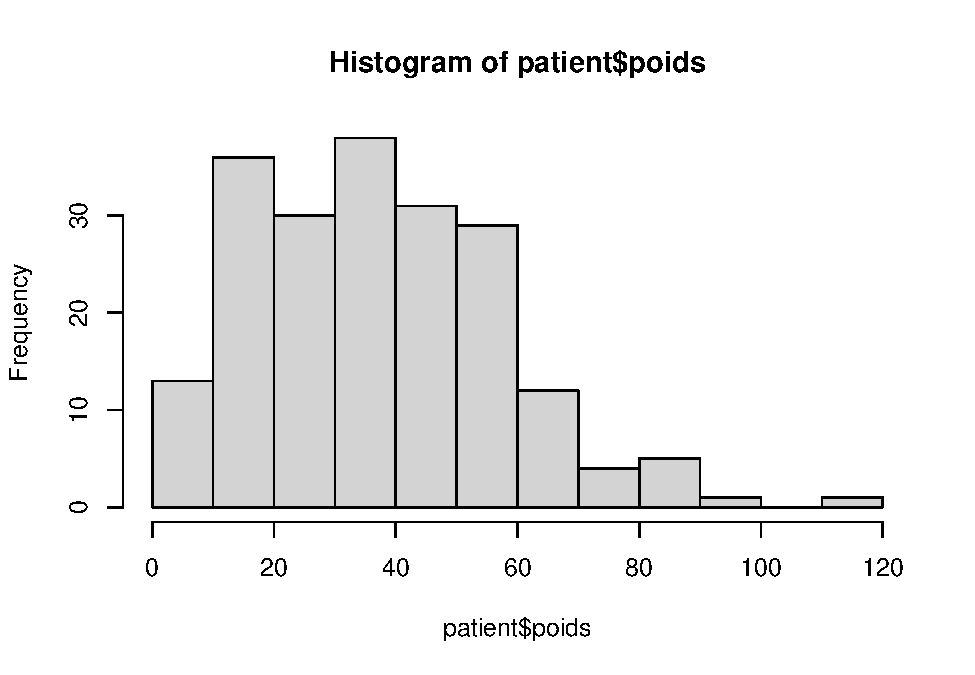
\includegraphics{_main_files/figure-latex/poids1-1.pdf}

Ce n'est pas très esthétique. Il y a des arguments aux fonctions qui permettent
d'améliorer les choses.

Déjà changer les noms des axes X et y, notamment se débarasser de \textbf{Frequency}
qui est un faux ami en français.

\begin{Shaded}
\begin{Highlighting}[]
\FunctionTok{hist}\NormalTok{(patient}\SpecialCharTok{$}\NormalTok{poids,}\AttributeTok{xlab=}\StringTok{"Poids"}\NormalTok{,}\AttributeTok{ylab=}\StringTok{"Effectifs"}\NormalTok{)}
\end{Highlighting}
\end{Shaded}

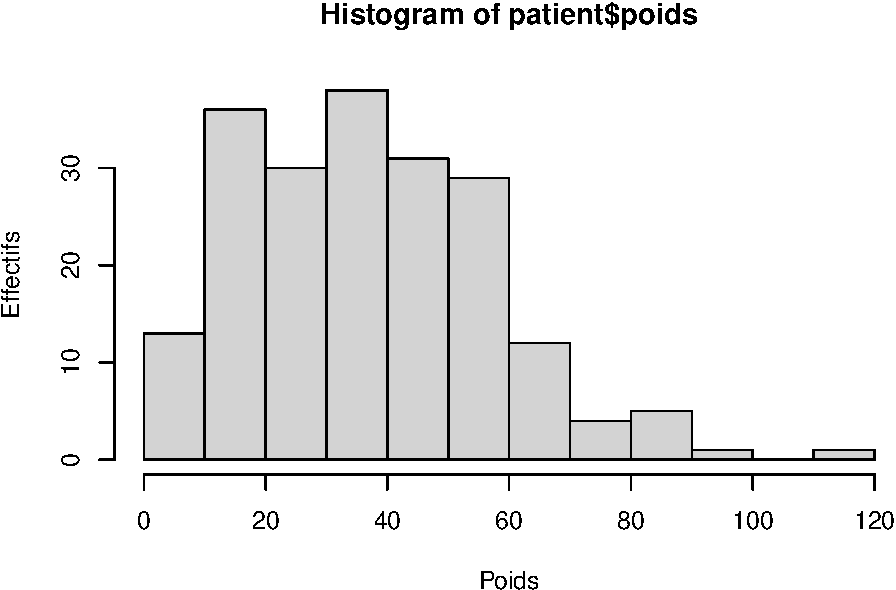
\includegraphics{_main_files/figure-latex/poids2-1.pdf}
Ensuite le titre :

\begin{Shaded}
\begin{Highlighting}[]
\FunctionTok{hist}\NormalTok{(patient}\SpecialCharTok{$}\NormalTok{poids,}\AttributeTok{xlab=}\StringTok{"Poids"}\NormalTok{,}\AttributeTok{ylab=}\StringTok{"Effectifs"}\NormalTok{,}\AttributeTok{main=}\StringTok{"Poids des patients"}\NormalTok{)}
\end{Highlighting}
\end{Shaded}

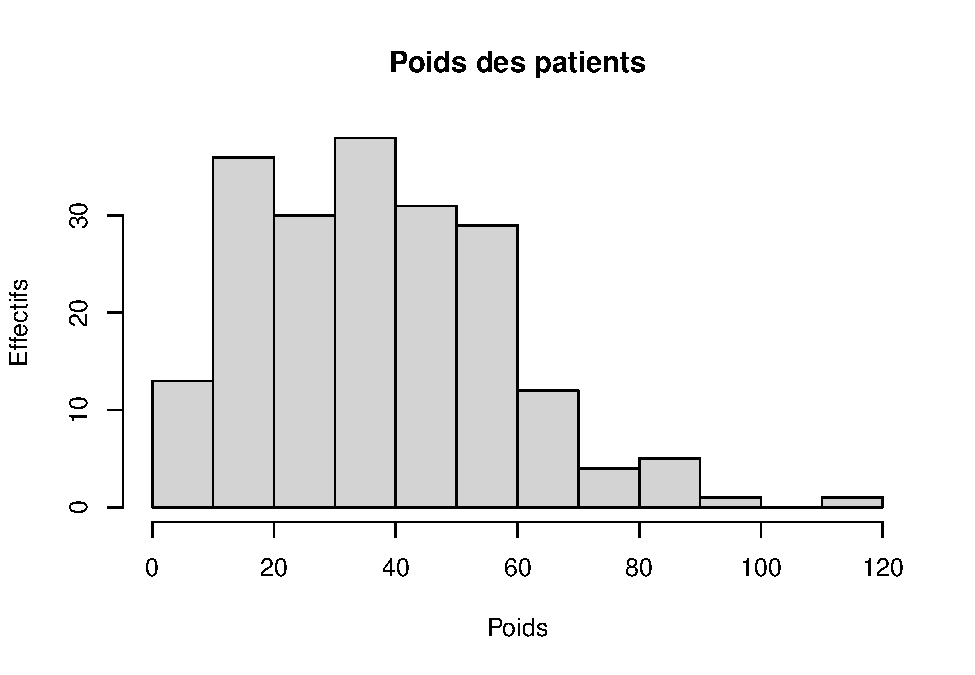
\includegraphics{_main_files/figure-latex/poids3-1.pdf}

Pour la couleur, c'est un peu plus compliqué. En effet il y a simple des couleurs
qui répondent à leurs mots en anglais, la liste est \href{https://www.datanovia.com/en/blog/awesome-list-of-657-r-color-names/}{là}.

Mais les couleurs correspondent au codage web des couleurs qui sont en fait des
hexadécimaux. Si vous voulez personnaliser plus les couleurs, je vous conseille
le paquet \textbf{RColorBrewer} qui possède de jolis (et intelligents) assortiments
de couleurs et \href{https://larmarange.github.io/analyse-R/couleurs.html}{de la lecture}

\begin{Shaded}
\begin{Highlighting}[]
\FunctionTok{hist}\NormalTok{(patient}\SpecialCharTok{$}\NormalTok{poids,}\AttributeTok{xlab=}\StringTok{"Poids"}\NormalTok{,}\AttributeTok{ylab=}\StringTok{"Effectifs"}\NormalTok{,}\AttributeTok{main=}\StringTok{"Poids des patients"}\NormalTok{,}\AttributeTok{col=}\StringTok{"lightblue"}\NormalTok{)}
\end{Highlighting}
\end{Shaded}

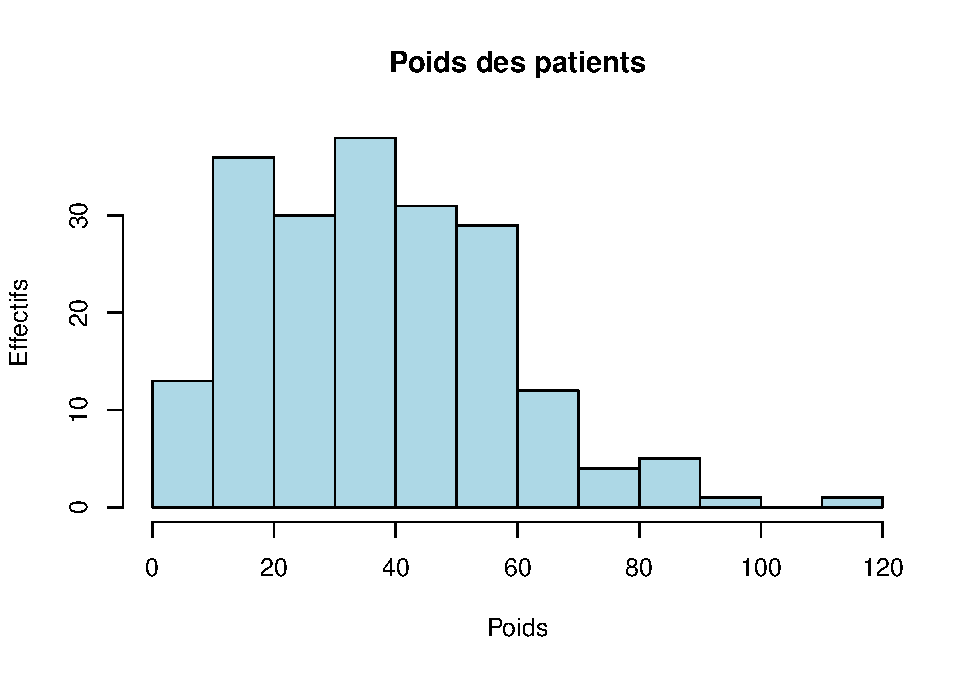
\includegraphics{_main_files/figure-latex/unnamed-chunk-74-1.pdf}
Ensuite il y a les boxplots ou boîtes à moustache pour les variables continues.

\begin{Shaded}
\begin{Highlighting}[]
\FunctionTok{boxplot}\NormalTok{(patient}\SpecialCharTok{$}\NormalTok{poids)}
\end{Highlighting}
\end{Shaded}

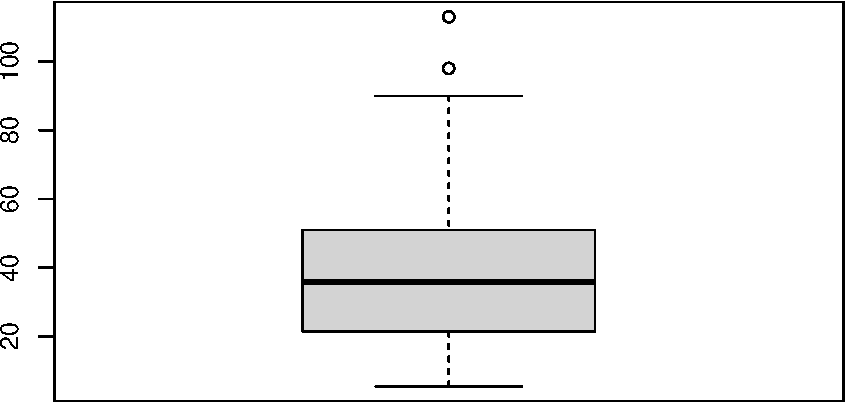
\includegraphics{_main_files/figure-latex/poids4-1.pdf}

De même on arrange un peu :

\begin{Shaded}
\begin{Highlighting}[]
\FunctionTok{boxplot}\NormalTok{(patient}\SpecialCharTok{$}\NormalTok{poids,}\AttributeTok{ylab=}\StringTok{"Poids"}\NormalTok{,}\AttributeTok{main=}\StringTok{"Poids des patients"}\NormalTok{)}
\end{Highlighting}
\end{Shaded}

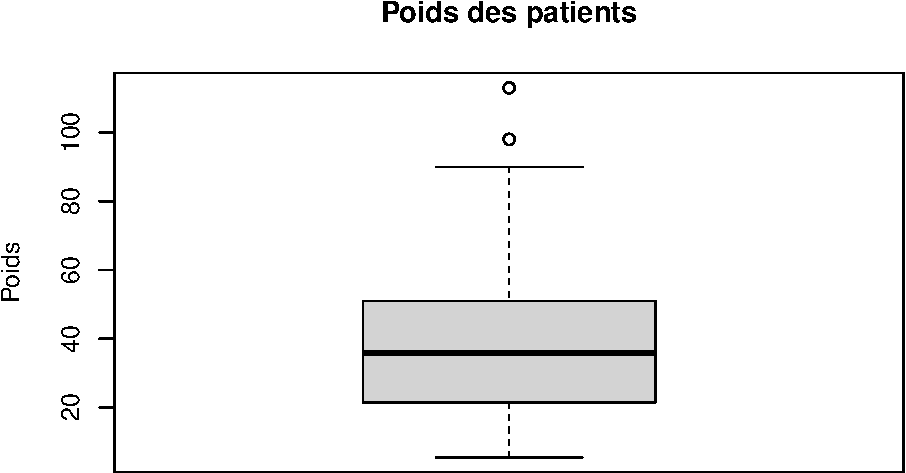
\includegraphics{_main_files/figure-latex/poids5-1.pdf}
Pour les boxplots on peut faire un peu mieux, par exemple pour segmenter par type
de pathologies.

On passe la \textbf{data.frame} patient et on précise le nom de la variable qualitative
qui doit ``séparer'' les tracés.

\begin{Shaded}
\begin{Highlighting}[]
\FunctionTok{boxplot}\NormalTok{(poids }\SpecialCharTok{\textasciitilde{}}\NormalTok{ CIM2, }\AttributeTok{data =}\NormalTok{ patient,}\AttributeTok{ylab=}\StringTok{"Poids"}\NormalTok{,}\AttributeTok{main=}\StringTok{"Poids des patients en fonction du CIM2"}\NormalTok{) }
\end{Highlighting}
\end{Shaded}

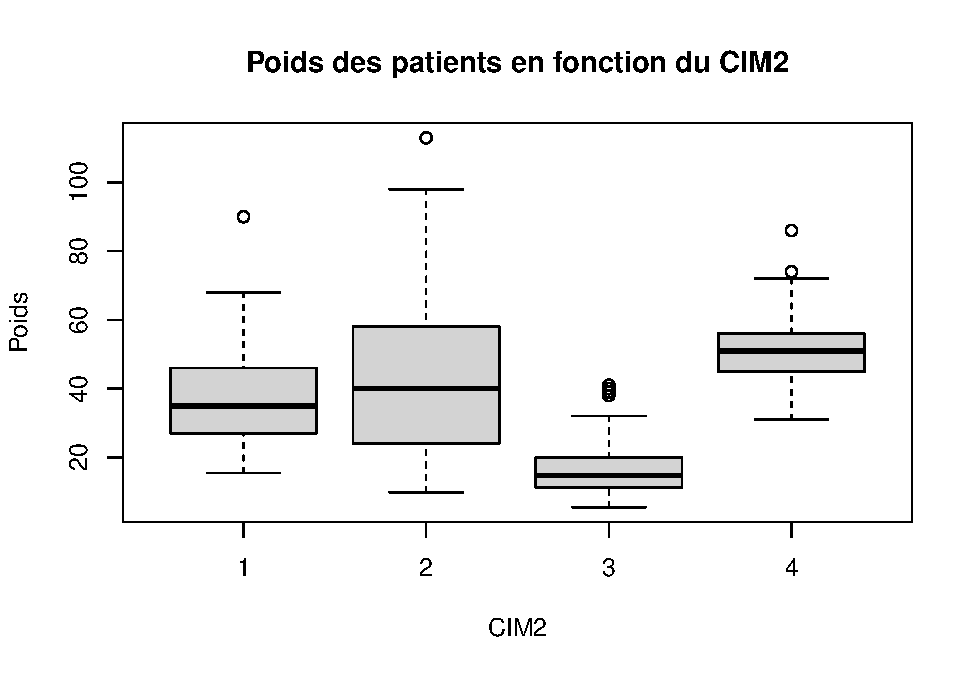
\includegraphics{_main_files/figure-latex/poids6-1.pdf}
Le premier argument doit vous paraître un peu abstrait. En fait c'est une formule
sous R. C'est l'équivalent de ``patient=CIM2''.

A gauche du \textasciitilde{} on place la variable à expliquer et à droite la ou les variables
explicatives. Ici on en a une de chaque côté.

Le graphique le plus simple serait le \textbf{scatterplot}. On aurait pu commencer
par lui :

Cette fois on a deux arguments qui sont la variable numérique des x en premier
et la variable numérique des y en second.

\begin{Shaded}
\begin{Highlighting}[]
\FunctionTok{plot}\NormalTok{(patient}\SpecialCharTok{$}\NormalTok{poids,patient}\SpecialCharTok{$}\NormalTok{dureeopmin)}
\end{Highlighting}
\end{Shaded}

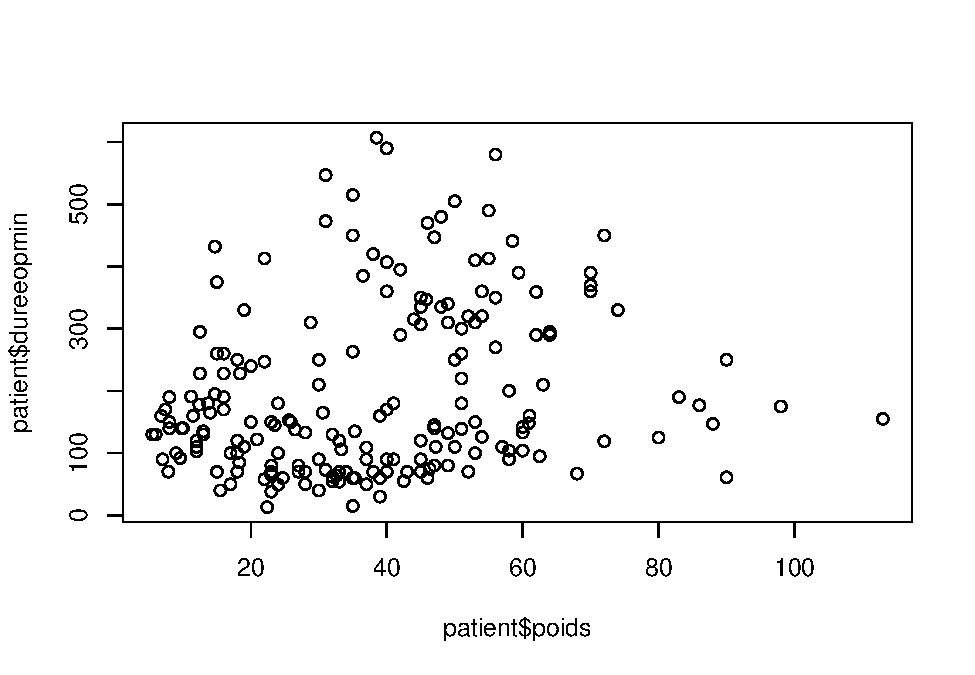
\includegraphics{_main_files/figure-latex/poids7-1.pdf}

\begin{Shaded}
\begin{Highlighting}[]
\FunctionTok{plot}\NormalTok{(patient}\SpecialCharTok{$}\NormalTok{poids,patient}\SpecialCharTok{$}\NormalTok{dureeopmin,}\AttributeTok{xlab=}\StringTok{"Poids"}\NormalTok{,}\AttributeTok{ylab=}\StringTok{"Durée opération en minutes"}\NormalTok{)}
\end{Highlighting}
\end{Shaded}

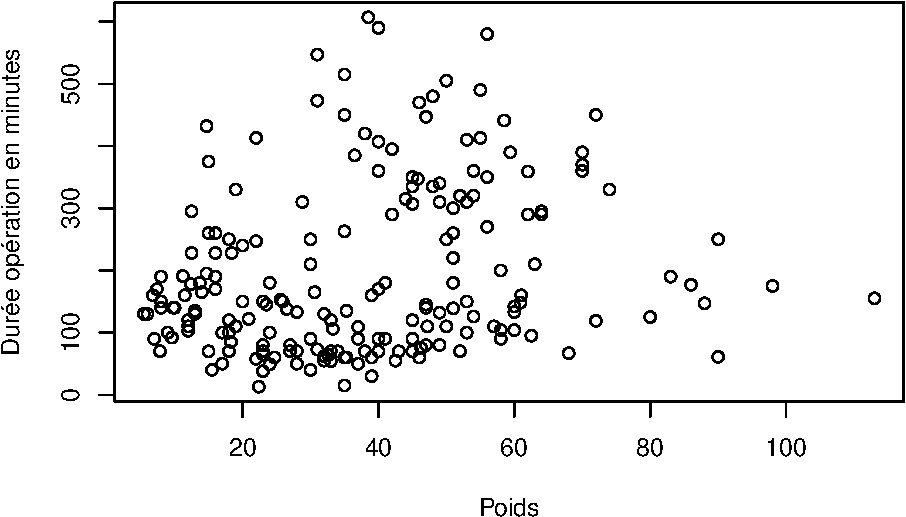
\includegraphics{_main_files/figure-latex/poids8-1.pdf}
Qui aurait pu s'écrire :

\begin{Shaded}
\begin{Highlighting}[]
\FunctionTok{plot}\NormalTok{(dureeopmin }\SpecialCharTok{\textasciitilde{}}\NormalTok{ poids,}\AttributeTok{data=}\NormalTok{patient,}\AttributeTok{xlab=}\StringTok{"Poids"}\NormalTok{,}\AttributeTok{ylab=}\StringTok{"Durée opération en minutes"}\NormalTok{)}
\end{Highlighting}
\end{Shaded}

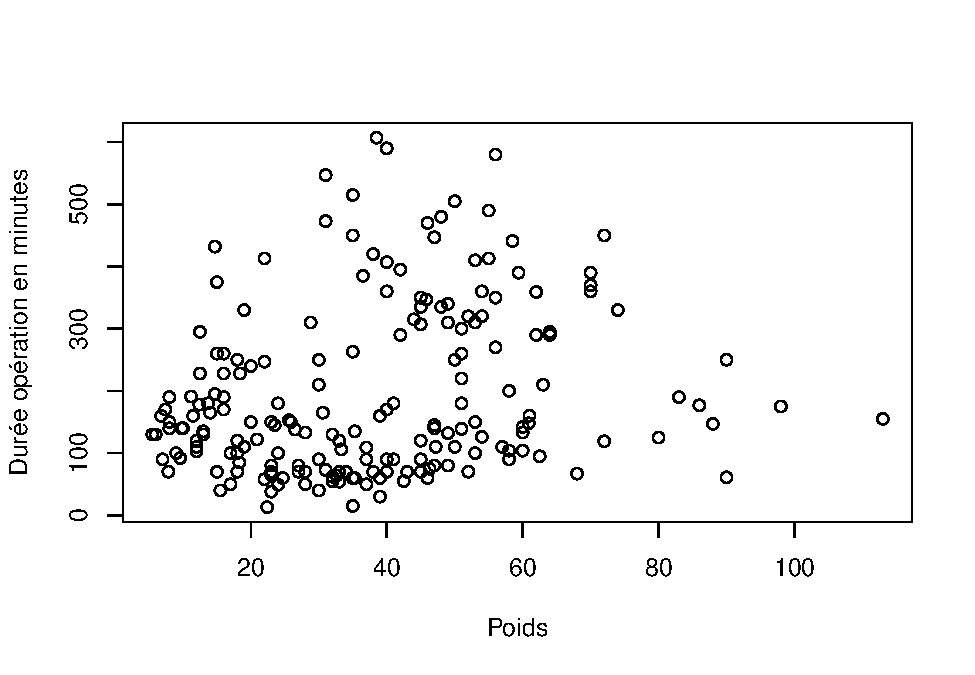
\includegraphics{_main_files/figure-latex/poids9-1.pdf}
Si on veut tracer une ligne pour la régression linéaire, il faut faire appel
à la fonction \textbf{lm} qui calcule la régression et R se charge du reste.

\begin{Shaded}
\begin{Highlighting}[]
\NormalTok{coefficients }\OtherTok{\textless{}{-}} \FunctionTok{lm}\NormalTok{(dureeopmin }\SpecialCharTok{\textasciitilde{}}\NormalTok{ poids,}\AttributeTok{data=}\NormalTok{patient)}
\FunctionTok{plot}\NormalTok{(patient}\SpecialCharTok{$}\NormalTok{poids,patient}\SpecialCharTok{$}\NormalTok{dureeopmin,}\AttributeTok{xlab=}\StringTok{"Poids"}\NormalTok{,}\AttributeTok{ylab=}\StringTok{"Durée opération en minutes"}\NormalTok{)}
\FunctionTok{abline}\NormalTok{(coefficients)}
\end{Highlighting}
\end{Shaded}

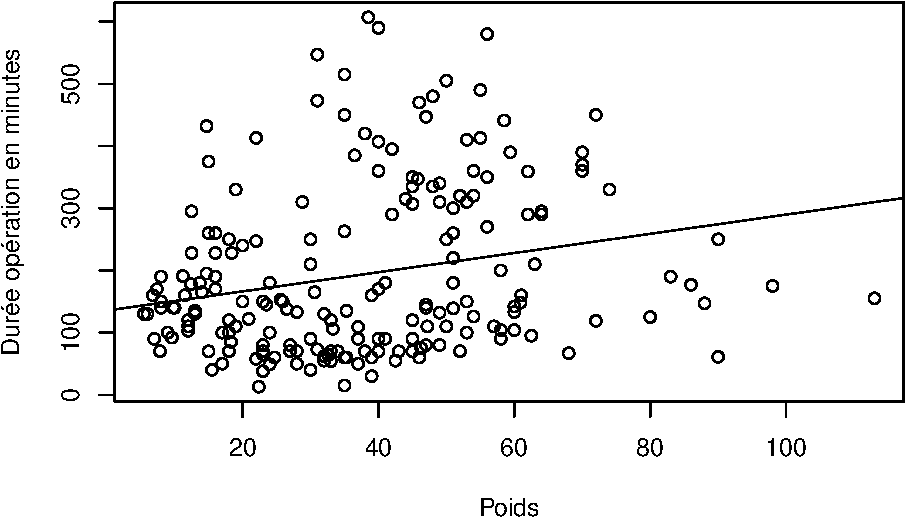
\includegraphics{_main_files/figure-latex/poids10-1.pdf}
On voit ici que j'ai appellé \textbf{abline} après le plot. En effet, il est nécessaire
de faire un \textbf{plot}, un \textbf{hist} ou une \textbf{boxplot} avant pour que R initialise
le graphique notamment le calcul des coordonnées maximales et minimales.

D'ailleurs on peut les spécifier nous mêmes :

\begin{Shaded}
\begin{Highlighting}[]
\NormalTok{coefficients }\OtherTok{\textless{}{-}} \FunctionTok{lm}\NormalTok{(dureeopmin}\SpecialCharTok{\textasciitilde{}}\NormalTok{poids,}\AttributeTok{data=}\NormalTok{patient)}
\FunctionTok{plot}\NormalTok{(patient}\SpecialCharTok{$}\NormalTok{poids,patient}\SpecialCharTok{$}\NormalTok{dureeopmin,}\AttributeTok{xlab=}\StringTok{"Poids"}\NormalTok{,}\AttributeTok{ylab=}\StringTok{"Durée opération en minutes"}\NormalTok{,}
     \AttributeTok{xlim=}\FunctionTok{c}\NormalTok{(}\DecValTok{0}\NormalTok{,}\DecValTok{150}\NormalTok{),}\AttributeTok{ylim=}\FunctionTok{c}\NormalTok{(}\DecValTok{0}\NormalTok{,}\DecValTok{600}\NormalTok{),}\AttributeTok{type=}\StringTok{"n"}\NormalTok{)}
\FunctionTok{abline}\NormalTok{(coefficients)}
\FunctionTok{text}\NormalTok{(patient}\SpecialCharTok{$}\NormalTok{poids,patient}\SpecialCharTok{$}\NormalTok{dureeopmin,patient}\SpecialCharTok{$}\NormalTok{UID)}
\end{Highlighting}
\end{Shaded}

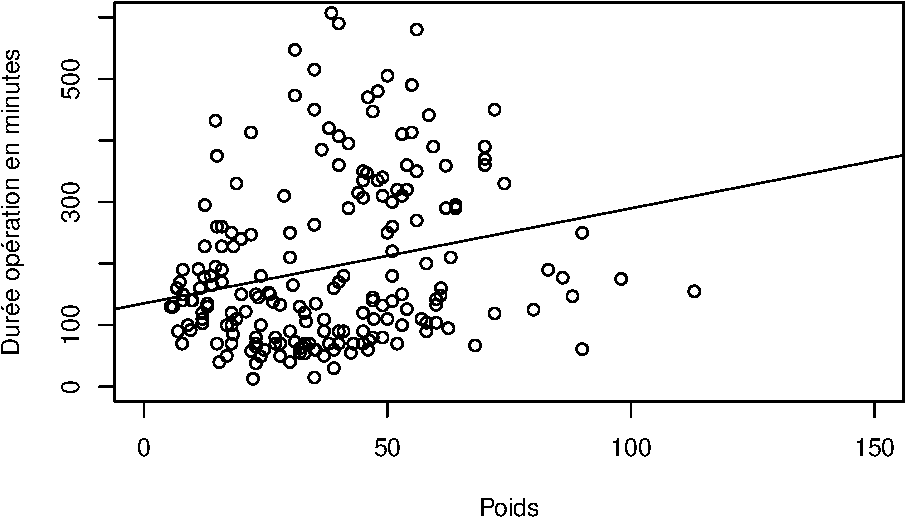
\includegraphics{_main_files/figure-latex/poids11-1.pdf}

Pour sauvegarder un graphique, on doit le faire avant d'appeler la fonction
\textbf{principale} et refermer le fichier avec la commande \textbf{dev.off}:

La dernière fonction à connaître pour les graphiques de base est le \textbf{barplot}.

Il s'agit de représenter des tableaux de contingence, le plus simple étant à une
dimension :

\begin{Shaded}
\begin{Highlighting}[]
\NormalTok{tableau }\OtherTok{\textless{}{-}} \FunctionTok{table}\NormalTok{(patient}\SpecialCharTok{$}\NormalTok{sexe)}
\FunctionTok{barplot}\NormalTok{(tableau, }\AttributeTok{main =} \StringTok{"sexe"}\NormalTok{, }\AttributeTok{ylab =} \StringTok{"Effectifs"}\NormalTok{)}
\end{Highlighting}
\end{Shaded}

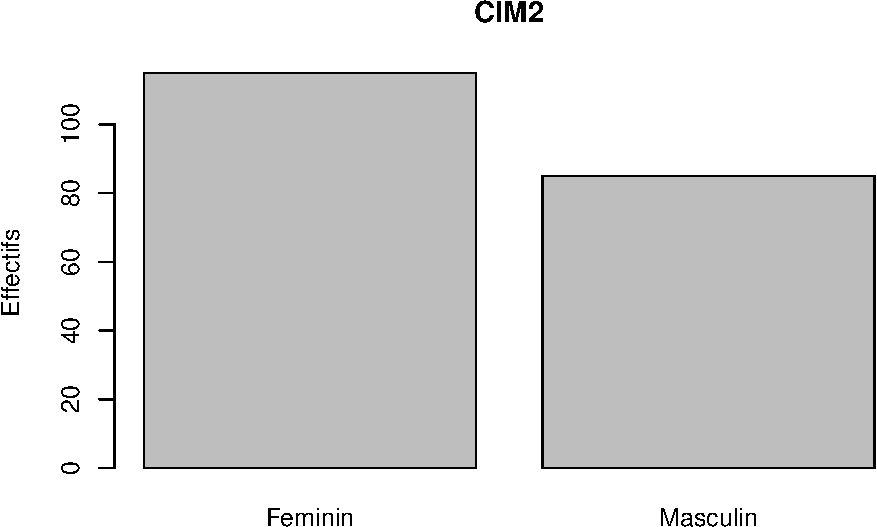
\includegraphics{_main_files/figure-latex/sexe1-1.pdf}
On peut lui passer un argument à deux dimensions mais la table devient tout de
suite difficile à lire.

\begin{Shaded}
\begin{Highlighting}[]
\NormalTok{tableau }\OtherTok{\textless{}{-}} \FunctionTok{table}\NormalTok{(patient}\SpecialCharTok{$}\NormalTok{CIM2,patient}\SpecialCharTok{$}\NormalTok{sexe)}
\FunctionTok{barplot}\NormalTok{(tableau, }\AttributeTok{main =} \StringTok{"CIM2"}\NormalTok{, }\AttributeTok{ylab =} \StringTok{"Effectifs"}\NormalTok{)}
\end{Highlighting}
\end{Shaded}

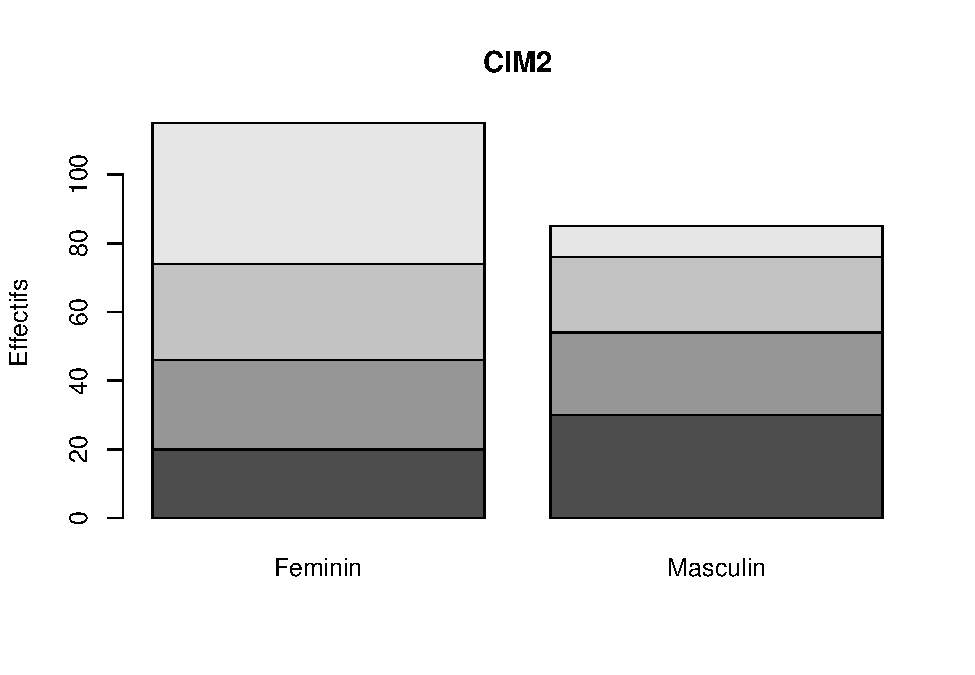
\includegraphics{_main_files/figure-latex/sexe2-1.pdf}

\hypertarget{le-tidyverse-et-ggplot}{%
\section{le tidyverse et ggplot}\label{le-tidyverse-et-ggplot}}

Vous pourrez comme précédemment entendre parler des graphiques de base de même
que des graphiques \textbf{lattice} mais le choucou du \textbf{tidyverse} c'est \textbf{ggplot2}.

C'est un éco-système de \textbf{packages} qui permet de faire la plupart des graphiques
plus simplement et qui est basé sur le paquet \textbf{gplot2}.

Un livre gratuit lui est consacré \href{https://ggplot2-book.org/}{là} et une page
en français \href{https://larmarange.github.io/analyse-R/graphiques-bivaries-ggplot2.html}{là}

On va reprendre notre grammaire. Il faut saisir que \textbf{ggplot2} fonctionne par
couche. Sur une base, vous additionner des couches qui apporte la personnalisation
des graphiques.

\hypertarget{la-base}{%
\subsection{La base}\label{la-base}}

Au tout départ, il faut lui passer une \textbf{data.frame}, c'est le passage obligé.

\begin{Shaded}
\begin{Highlighting}[]
\FunctionTok{ggplot}\NormalTok{(patient)}
\end{Highlighting}
\end{Shaded}


\includegraphics{_main_files/figure-latex/ggplot1-1.pdf}
Ensuite on précise les variables de travail. Pour l'histogramme, on en a qu'une :

\begin{Shaded}
\begin{Highlighting}[]
\FunctionTok{ggplot}\NormalTok{(patient,}\FunctionTok{aes}\NormalTok{(poids))}
\end{Highlighting}
\end{Shaded}

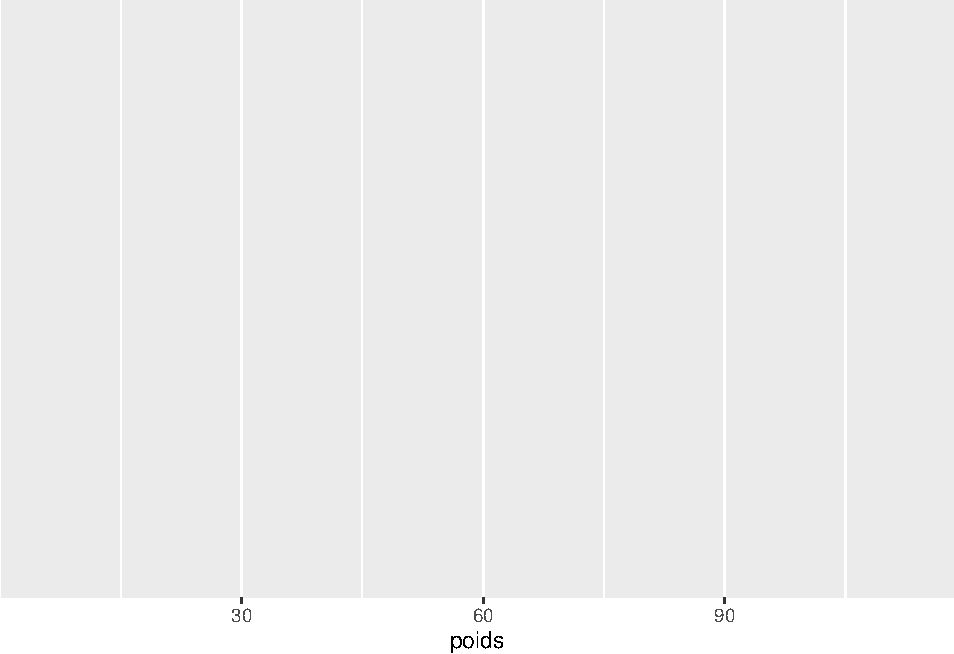
\includegraphics{_main_files/figure-latex/ggplot2-1.pdf}

Vous pouvez constater, que le logiciel a calculé et positionner les légendes
pour créer un graphique avec poids comme variable des abscisses (horizontal).

On personnalise en demandant un graphique de type histogramme. En additionnant
littéralement:

\begin{Shaded}
\begin{Highlighting}[]
\FunctionTok{ggplot}\NormalTok{(patient,}\FunctionTok{aes}\NormalTok{(poids))}\SpecialCharTok{+}\FunctionTok{geom\_histogram}\NormalTok{()}
\end{Highlighting}
\end{Shaded}

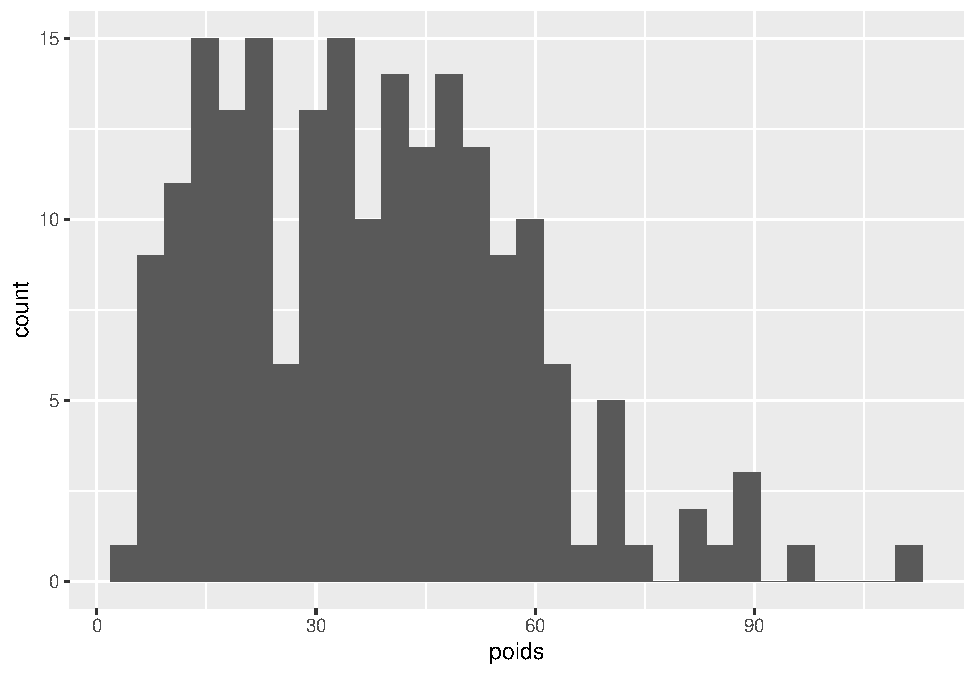
\includegraphics{_main_files/figure-latex/ggplot3-1.pdf}

Pour modifier les limtes du graphiques, on rajoute :

\begin{Shaded}
\begin{Highlighting}[]
\FunctionTok{ggplot}\NormalTok{(patient,}\FunctionTok{aes}\NormalTok{(poids))}\SpecialCharTok{+}\FunctionTok{geom\_histogram}\NormalTok{()}\SpecialCharTok{+}
  \FunctionTok{scale\_x\_continuous}\NormalTok{(}\AttributeTok{limits =} \FunctionTok{c}\NormalTok{(}\DecValTok{0}\NormalTok{,}\DecValTok{150}\NormalTok{)) }\SpecialCharTok{+}
  \FunctionTok{scale\_y\_continuous}\NormalTok{(}\AttributeTok{limits =} \FunctionTok{c}\NormalTok{(}\DecValTok{0}\NormalTok{,}\DecValTok{20}\NormalTok{))}
\end{Highlighting}
\end{Shaded}

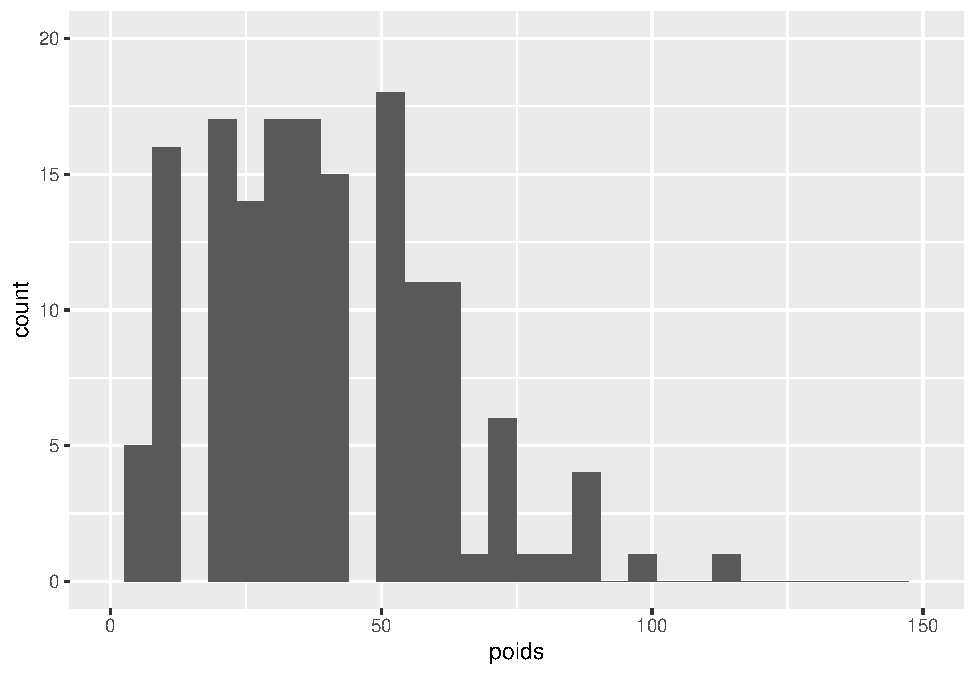
\includegraphics{_main_files/figure-latex/ggplot4-1.pdf}

Si on veut modifier le nombre de barres verticales (la précision de l'histogramme),
on précise l'option dans la couche de l'histogramme :

\begin{Shaded}
\begin{Highlighting}[]
\FunctionTok{ggplot}\NormalTok{(patient,}\FunctionTok{aes}\NormalTok{(poids))}\SpecialCharTok{+}\FunctionTok{geom\_histogram}\NormalTok{(}\AttributeTok{bins=}\DecValTok{10}\NormalTok{)}\SpecialCharTok{+}
  \FunctionTok{scale\_x\_continuous}\NormalTok{(}\AttributeTok{limits =} \FunctionTok{c}\NormalTok{(}\DecValTok{0}\NormalTok{,}\DecValTok{150}\NormalTok{))}
\end{Highlighting}
\end{Shaded}

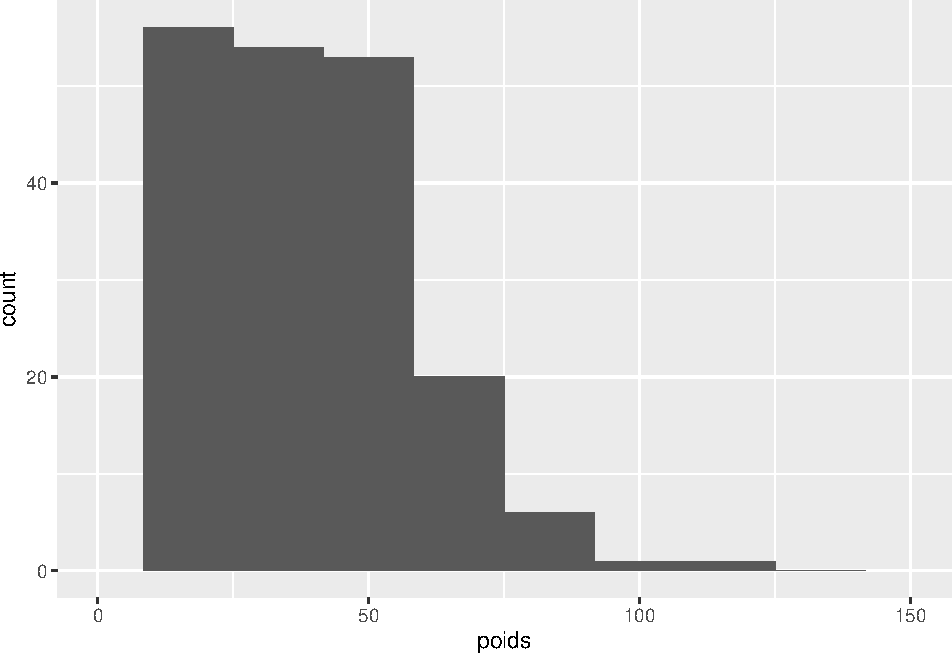
\includegraphics{_main_files/figure-latex/ggplot5-1.pdf}
Pour les titres, c'est pareil, on ajoute des couches :

\begin{Shaded}
\begin{Highlighting}[]
\FunctionTok{ggplot}\NormalTok{(patient,}\FunctionTok{aes}\NormalTok{(poids))}\SpecialCharTok{+}\FunctionTok{geom\_histogram}\NormalTok{()}\SpecialCharTok{+}
  \FunctionTok{scale\_x\_continuous}\NormalTok{(}\AttributeTok{limits =} \FunctionTok{c}\NormalTok{(}\DecValTok{0}\NormalTok{,}\DecValTok{150}\NormalTok{)) }\SpecialCharTok{+} 
  \FunctionTok{ggtitle}\NormalTok{(}\StringTok{"Poids des patients"}\NormalTok{) }\SpecialCharTok{+} 
  \FunctionTok{xlab}\NormalTok{(}\StringTok{"Poids"}\NormalTok{) }\SpecialCharTok{+} 
  \FunctionTok{ylab}\NormalTok{(}\StringTok{"Effectifs"}\NormalTok{)}
\end{Highlighting}
\end{Shaded}

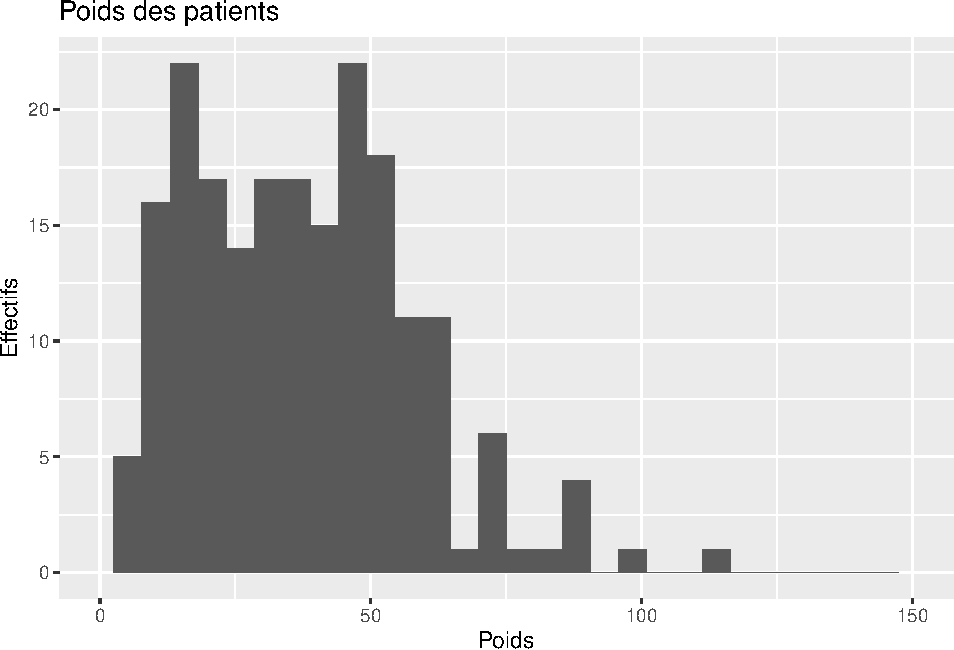
\includegraphics{_main_files/figure-latex/ggplot6-1.pdf}
On peut ajouter des propriétés esthétiques comme la couleur, par exemple :

\begin{Shaded}
\begin{Highlighting}[]
\FunctionTok{ggplot}\NormalTok{(patient,}\FunctionTok{aes}\NormalTok{(poids))}\SpecialCharTok{+}\FunctionTok{geom\_histogram}\NormalTok{(}\AttributeTok{fill =}\StringTok{"lightblue"}\NormalTok{, }\AttributeTok{colour =} \StringTok{"black"}\NormalTok{)}\SpecialCharTok{+}
  \FunctionTok{scale\_x\_continuous}\NormalTok{(}\AttributeTok{limits =} \FunctionTok{c}\NormalTok{(}\DecValTok{0}\NormalTok{,}\DecValTok{150}\NormalTok{)) }\SpecialCharTok{+} 
  \FunctionTok{ggtitle}\NormalTok{(}\StringTok{"Poids des patients"}\NormalTok{) }\SpecialCharTok{+} 
  \FunctionTok{xlab}\NormalTok{(}\StringTok{"Poids"}\NormalTok{) }\SpecialCharTok{+} 
  \FunctionTok{ylab}\NormalTok{(}\StringTok{"Effectifs"}\NormalTok{)}
\end{Highlighting}
\end{Shaded}

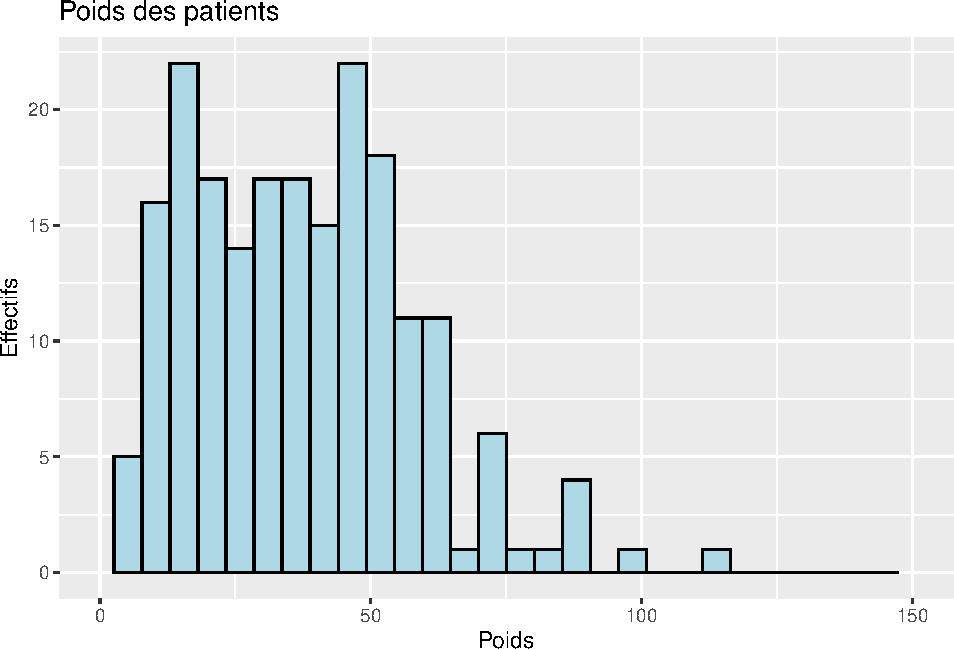
\includegraphics{_main_files/figure-latex/ggplot7-1.pdf}

Là où \textbf{ggplot2} sort du lot, c'est sa capacité à segmenter et à représenter
avec \href{https://link.springer.com/book/10.1007/0-387-28695-0}{une bonne grammaire graphique}

\begin{Shaded}
\begin{Highlighting}[]
\FunctionTok{ggplot}\NormalTok{(patient,}\FunctionTok{aes}\NormalTok{(poids,}\AttributeTok{fill=}\NormalTok{sexe))}\SpecialCharTok{+}\FunctionTok{geom\_histogram}\NormalTok{(}\AttributeTok{color=}\StringTok{"black"}\NormalTok{)}\SpecialCharTok{+}
  \FunctionTok{scale\_x\_continuous}\NormalTok{(}\AttributeTok{limits =} \FunctionTok{c}\NormalTok{(}\DecValTok{0}\NormalTok{,}\DecValTok{150}\NormalTok{)) }\SpecialCharTok{+} 
  \FunctionTok{ggtitle}\NormalTok{(}\StringTok{"Poids des patients"}\NormalTok{) }\SpecialCharTok{+} 
  \FunctionTok{xlab}\NormalTok{(}\StringTok{"Poids"}\NormalTok{) }\SpecialCharTok{+} 
  \FunctionTok{ylab}\NormalTok{(}\StringTok{"Effectifs"}\NormalTok{)}
\end{Highlighting}
\end{Shaded}

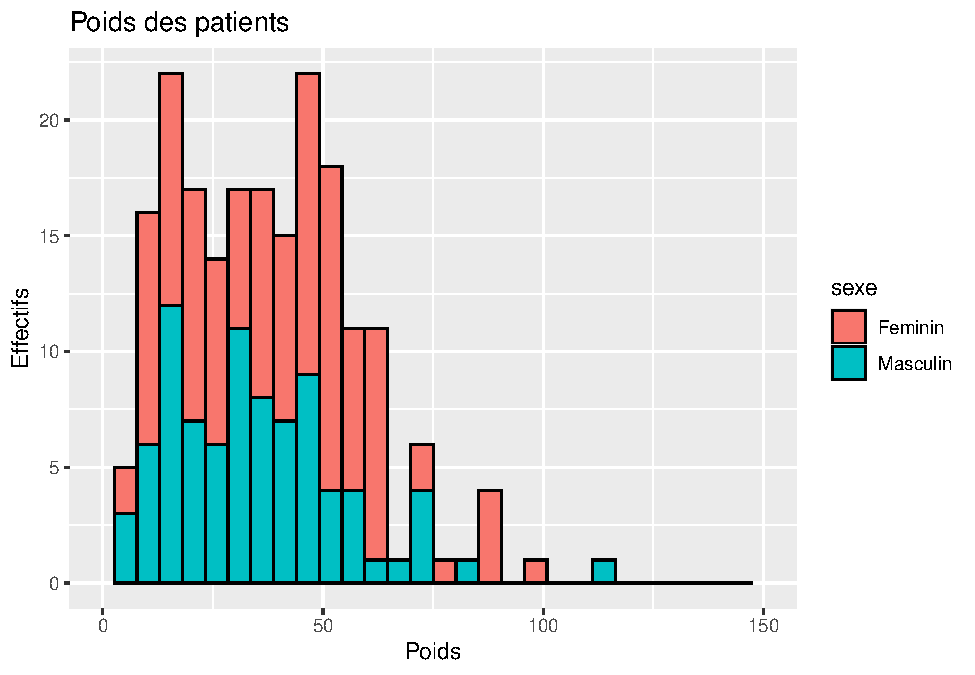
\includegraphics{_main_files/figure-latex/ggplot8-1.pdf}

On a l'ajout de couleurs ou alors deux graphiques avec des unités bien choisies:

\begin{Shaded}
\begin{Highlighting}[]
\FunctionTok{ggplot}\NormalTok{(patient,}\FunctionTok{aes}\NormalTok{(poids,}\AttributeTok{fill=}\NormalTok{sexe))}\SpecialCharTok{+}\FunctionTok{geom\_histogram}\NormalTok{(}\AttributeTok{color=}\StringTok{"black"}\NormalTok{)}\SpecialCharTok{+}
  \FunctionTok{scale\_x\_continuous}\NormalTok{(}\AttributeTok{limits =} \FunctionTok{c}\NormalTok{(}\DecValTok{0}\NormalTok{,}\DecValTok{150}\NormalTok{)) }\SpecialCharTok{+} 
  \FunctionTok{ggtitle}\NormalTok{(}\StringTok{"Poids des patients"}\NormalTok{) }\SpecialCharTok{+} 
  \FunctionTok{xlab}\NormalTok{(}\StringTok{"Poids"}\NormalTok{) }\SpecialCharTok{+} 
  \FunctionTok{ylab}\NormalTok{(}\StringTok{"Effectifs"}\NormalTok{) }\SpecialCharTok{+}
  \FunctionTok{facet\_grid}\NormalTok{(sexe }\SpecialCharTok{\textasciitilde{}}\NormalTok{ .)}
\end{Highlighting}
\end{Shaded}

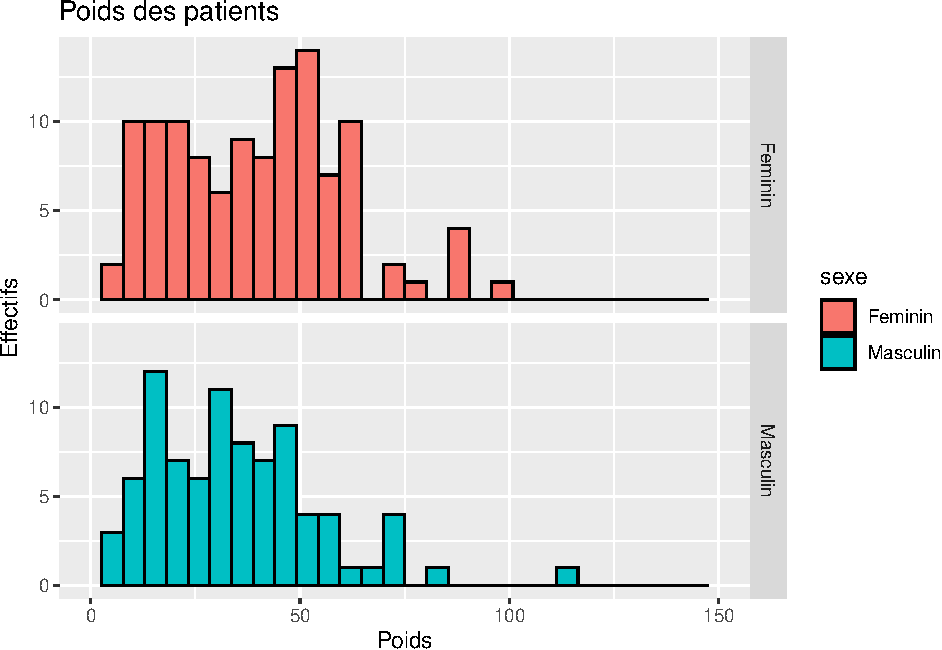
\includegraphics{_main_files/figure-latex/ggplot9-1.pdf}

On a de nouveau une formule. Cette fois, c'est à gauche du \textasciitilde{} les lignes et
à droite les colonnes :

\begin{Shaded}
\begin{Highlighting}[]
\FunctionTok{ggplot}\NormalTok{(patient,}\FunctionTok{aes}\NormalTok{(poids))}\SpecialCharTok{+}\FunctionTok{geom\_histogram}\NormalTok{(}\AttributeTok{color=}\StringTok{"black"}\NormalTok{)}\SpecialCharTok{+}
  \FunctionTok{scale\_x\_continuous}\NormalTok{(}\AttributeTok{limits =} \FunctionTok{c}\NormalTok{(}\DecValTok{0}\NormalTok{,}\DecValTok{150}\NormalTok{)) }\SpecialCharTok{+} 
  \FunctionTok{ggtitle}\NormalTok{(}\StringTok{"Poids des patients"}\NormalTok{) }\SpecialCharTok{+} 
  \FunctionTok{xlab}\NormalTok{(}\StringTok{"Poids"}\NormalTok{) }\SpecialCharTok{+} 
  \FunctionTok{ylab}\NormalTok{(}\StringTok{"Effectifs"}\NormalTok{) }\SpecialCharTok{+}
  \FunctionTok{facet\_grid}\NormalTok{(sexe }\SpecialCharTok{\textasciitilde{}}\NormalTok{ Hopital)}
\end{Highlighting}
\end{Shaded}

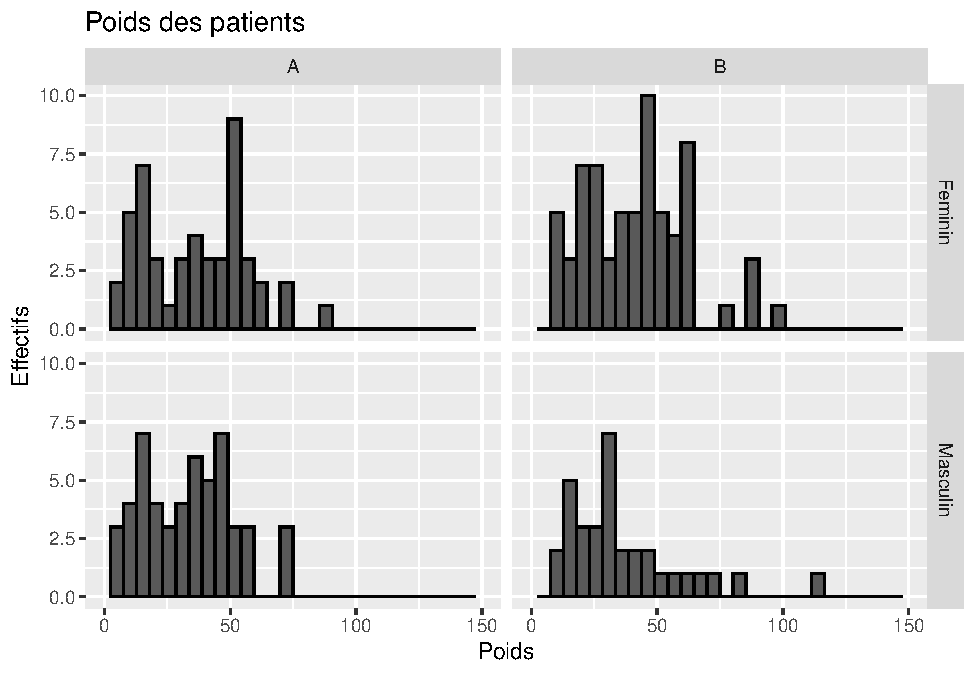
\includegraphics{_main_files/figure-latex/ggplot10-1.pdf}

On peut vouloir calculer la \textbf{densité} et non les effectifs dans ce cas :

\begin{Shaded}
\begin{Highlighting}[]
\FunctionTok{ggplot}\NormalTok{(patient,}\FunctionTok{aes}\NormalTok{(poids))}\SpecialCharTok{+}\FunctionTok{geom\_histogram}\NormalTok{(}\FunctionTok{aes}\NormalTok{(}\AttributeTok{y =}\NormalTok{ ..density..),}\AttributeTok{color=}\StringTok{"black"}\NormalTok{)}\SpecialCharTok{+}
  \FunctionTok{scale\_x\_continuous}\NormalTok{(}\AttributeTok{limits =} \FunctionTok{c}\NormalTok{(}\DecValTok{0}\NormalTok{,}\DecValTok{150}\NormalTok{)) }\SpecialCharTok{+} 
  \FunctionTok{ggtitle}\NormalTok{(}\StringTok{"Poids des patients"}\NormalTok{) }\SpecialCharTok{+} 
  \FunctionTok{xlab}\NormalTok{(}\StringTok{"Poids"}\NormalTok{) }\SpecialCharTok{+} 
  \FunctionTok{ylab}\NormalTok{(}\StringTok{"Densité"}\NormalTok{) }\SpecialCharTok{+}
  \FunctionTok{facet\_grid}\NormalTok{(sexe }\SpecialCharTok{\textasciitilde{}}\NormalTok{ Hopital)}
\end{Highlighting}
\end{Shaded}

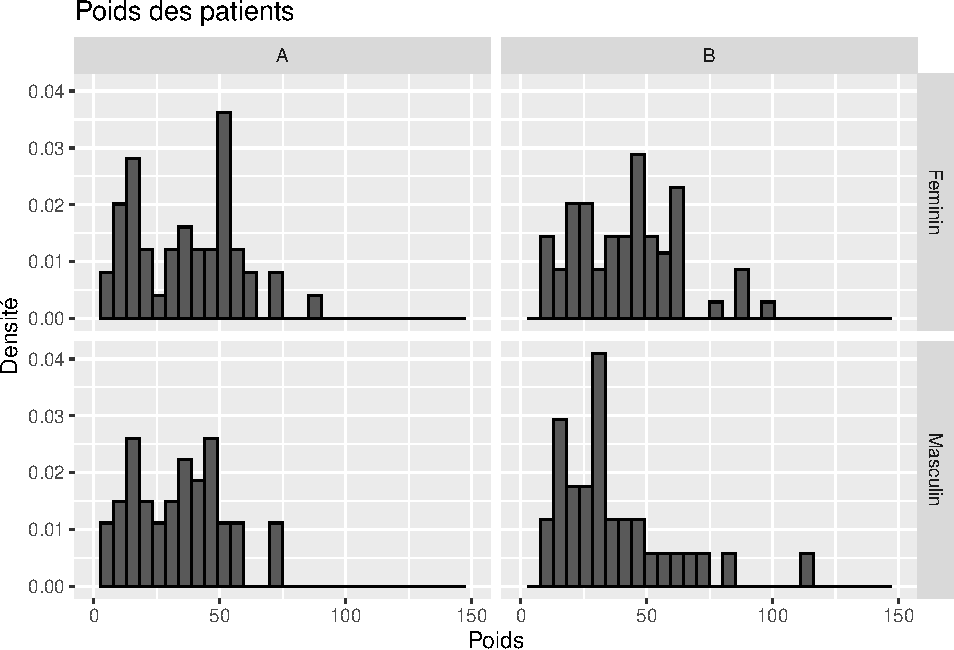
\includegraphics{_main_files/figure-latex/ggplot11-1.pdf}

\hypertarget{les-autres-graphiques}{%
\subsection{Les autres graphiques}\label{les-autres-graphiques}}

Le boxplot :

\begin{Shaded}
\begin{Highlighting}[]
\FunctionTok{ggplot}\NormalTok{(patient,}\FunctionTok{aes}\NormalTok{(}\AttributeTok{x=}\NormalTok{poids,}\AttributeTok{fill=}\NormalTok{sexe))}\SpecialCharTok{+}\FunctionTok{geom\_boxplot}\NormalTok{()}\SpecialCharTok{+}
  \FunctionTok{ggtitle}\NormalTok{(}\StringTok{"Poids des patients"}\NormalTok{) }\SpecialCharTok{+} 
  \FunctionTok{xlab}\NormalTok{(}\StringTok{"Poids"}\NormalTok{) }\SpecialCharTok{+} 
  \FunctionTok{ylab}\NormalTok{(}\StringTok{"Densité"}\NormalTok{) }\SpecialCharTok{+}
  \FunctionTok{facet\_grid}\NormalTok{(Hopital }\SpecialCharTok{\textasciitilde{}}\NormalTok{ .)}
\end{Highlighting}
\end{Shaded}

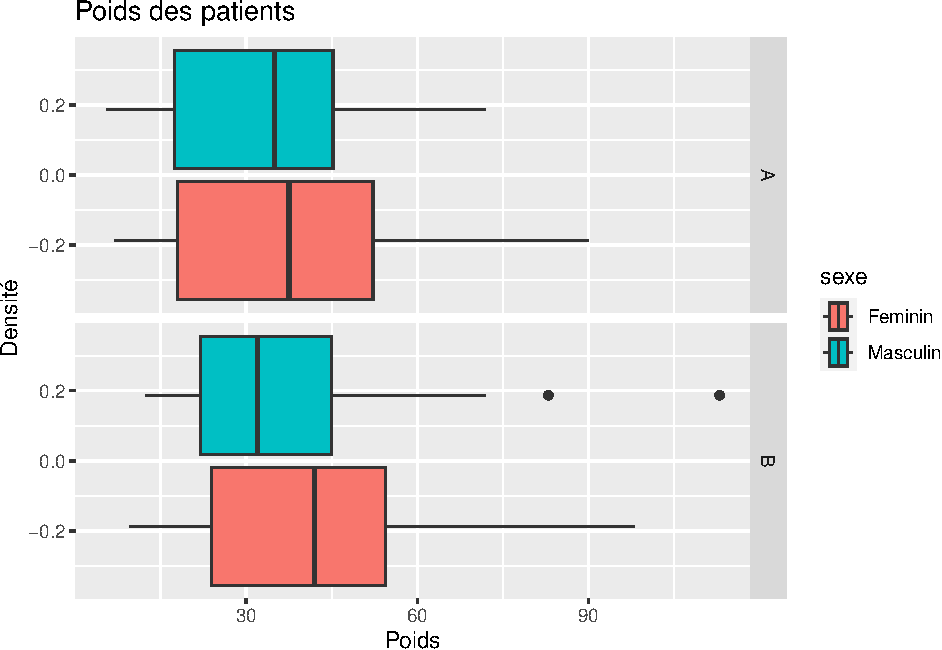
\includegraphics{_main_files/figure-latex/ggplot12-1.pdf}

\begin{Shaded}
\begin{Highlighting}[]
\FunctionTok{ggplot}\NormalTok{(patient,}\FunctionTok{aes}\NormalTok{(}\AttributeTok{x=}\NormalTok{sexe,}\AttributeTok{y=}\NormalTok{poids))}\SpecialCharTok{+}\FunctionTok{geom\_boxplot}\NormalTok{()}\SpecialCharTok{+}
  \FunctionTok{ggtitle}\NormalTok{(}\StringTok{"Poids des patients"}\NormalTok{) }\SpecialCharTok{+} 
  \FunctionTok{xlab}\NormalTok{(}\StringTok{"Poids"}\NormalTok{) }\SpecialCharTok{+} 
  \FunctionTok{ylab}\NormalTok{(}\StringTok{"Densité"}\NormalTok{) }\SpecialCharTok{+}
  \FunctionTok{facet\_grid}\NormalTok{(Hopital }\SpecialCharTok{\textasciitilde{}}\NormalTok{ .)}
\end{Highlighting}
\end{Shaded}

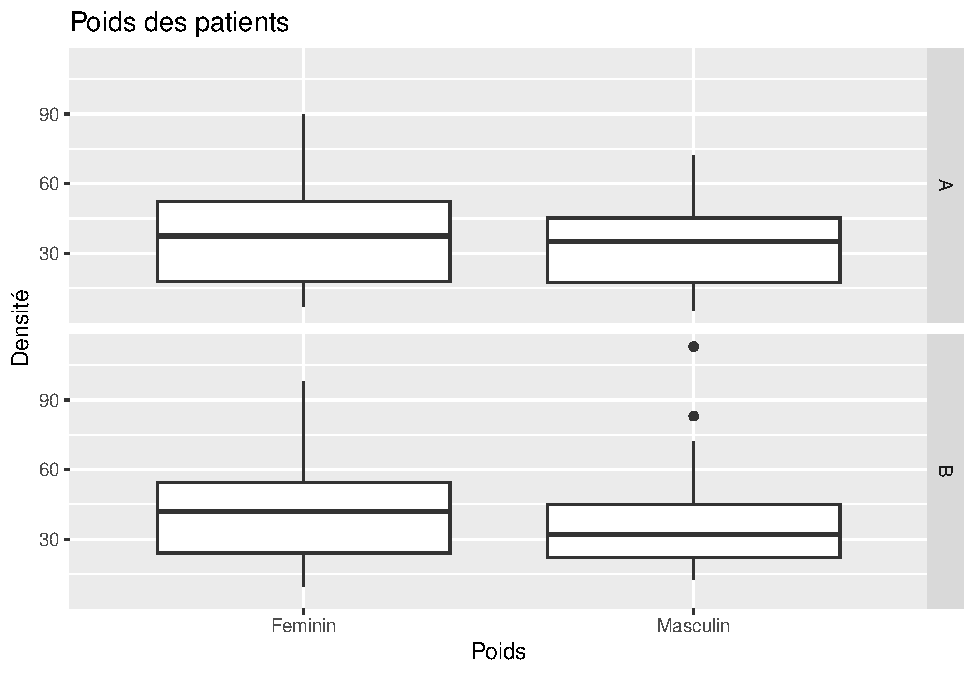
\includegraphics{_main_files/figure-latex/ggplot13-1.pdf}

\begin{Shaded}
\begin{Highlighting}[]
\FunctionTok{ggplot}\NormalTok{(patient,}\FunctionTok{aes}\NormalTok{(poids))}\SpecialCharTok{+}\FunctionTok{geom\_boxplot}\NormalTok{()}\SpecialCharTok{+}
  \FunctionTok{ggtitle}\NormalTok{(}\StringTok{"Poids des patients"}\NormalTok{) }\SpecialCharTok{+} 
  \FunctionTok{xlab}\NormalTok{(}\StringTok{"Poids"}\NormalTok{) }\SpecialCharTok{+} 
  \FunctionTok{ylab}\NormalTok{(}\StringTok{"Densité"}\NormalTok{) }\SpecialCharTok{+}
  \FunctionTok{facet\_grid}\NormalTok{(sexe }\SpecialCharTok{\textasciitilde{}}\NormalTok{ Hopital)}
\end{Highlighting}
\end{Shaded}

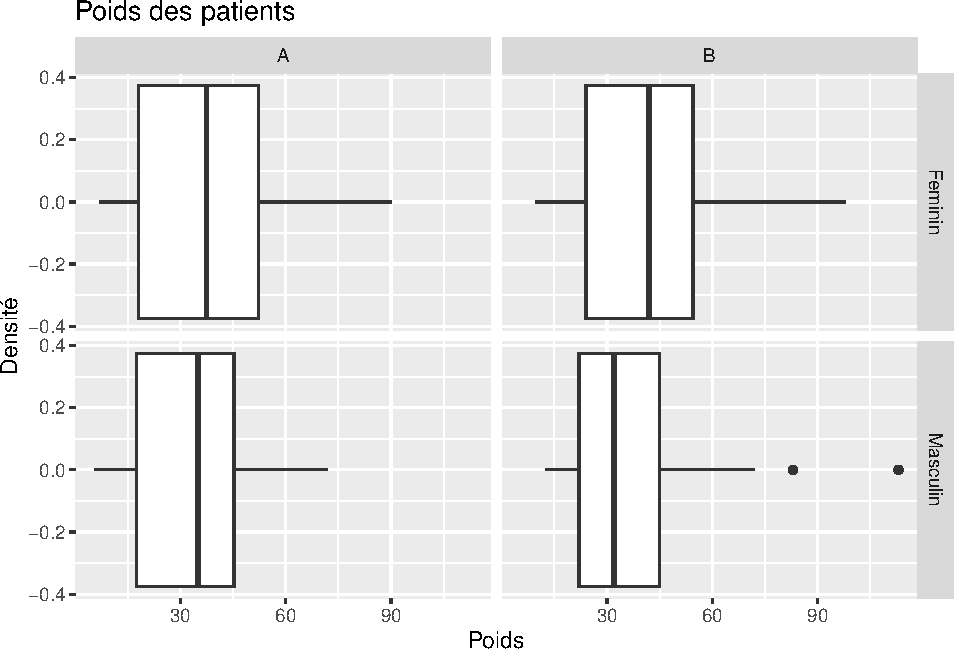
\includegraphics{_main_files/figure-latex/ggplot14-1.pdf}

D'où des graphiques en \textbf{scatterplot} comme :

\begin{Shaded}
\begin{Highlighting}[]
\FunctionTok{ggplot}\NormalTok{(patient,}\FunctionTok{aes}\NormalTok{(}\AttributeTok{x=}\NormalTok{poids,}\AttributeTok{y=}\NormalTok{dureeopmin))}\SpecialCharTok{+}\FunctionTok{geom\_point}\NormalTok{(}\FunctionTok{aes}\NormalTok{(}\AttributeTok{col=}\NormalTok{sexe))}\SpecialCharTok{+}
  \FunctionTok{ggtitle}\NormalTok{(}\StringTok{"Caractéristiques des patients"}\NormalTok{) }\SpecialCharTok{+} 
  \FunctionTok{xlab}\NormalTok{(}\StringTok{"Poids"}\NormalTok{) }\SpecialCharTok{+} 
  \FunctionTok{ylab}\NormalTok{(}\StringTok{"Durée de l\textquotesingle{}opération en minutes"}\NormalTok{) }
\end{Highlighting}
\end{Shaded}

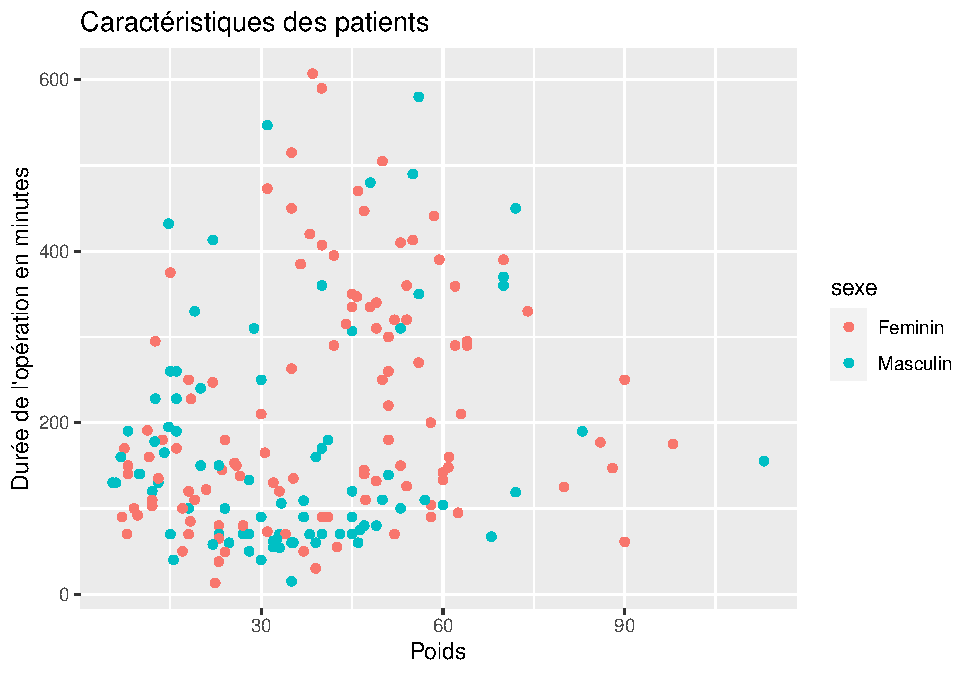
\includegraphics{_main_files/figure-latex/ggplot15-1.pdf}

ou en rajoutant plein de trucs :

\begin{Shaded}
\begin{Highlighting}[]
\FunctionTok{ggplot}\NormalTok{(patient,}\FunctionTok{aes}\NormalTok{(}\AttributeTok{x=}\NormalTok{poids,}\AttributeTok{y=}\NormalTok{dureeopmin))}\SpecialCharTok{+}\FunctionTok{geom\_point}\NormalTok{(}\FunctionTok{aes}\NormalTok{(}\AttributeTok{col=}\NormalTok{sexe))}\SpecialCharTok{+}
  \FunctionTok{ggtitle}\NormalTok{(}\StringTok{"Caractéristiques des patients"}\NormalTok{) }\SpecialCharTok{+} 
  \FunctionTok{xlab}\NormalTok{(}\StringTok{"Poids"}\NormalTok{) }\SpecialCharTok{+} 
  \FunctionTok{ylab}\NormalTok{(}\StringTok{"Durée de l\textquotesingle{}opération en minutes"}\NormalTok{) }\SpecialCharTok{+}
  \FunctionTok{facet\_grid}\NormalTok{(CIM2 }\SpecialCharTok{\textasciitilde{}}\NormalTok{ Hopital)}
\end{Highlighting}
\end{Shaded}

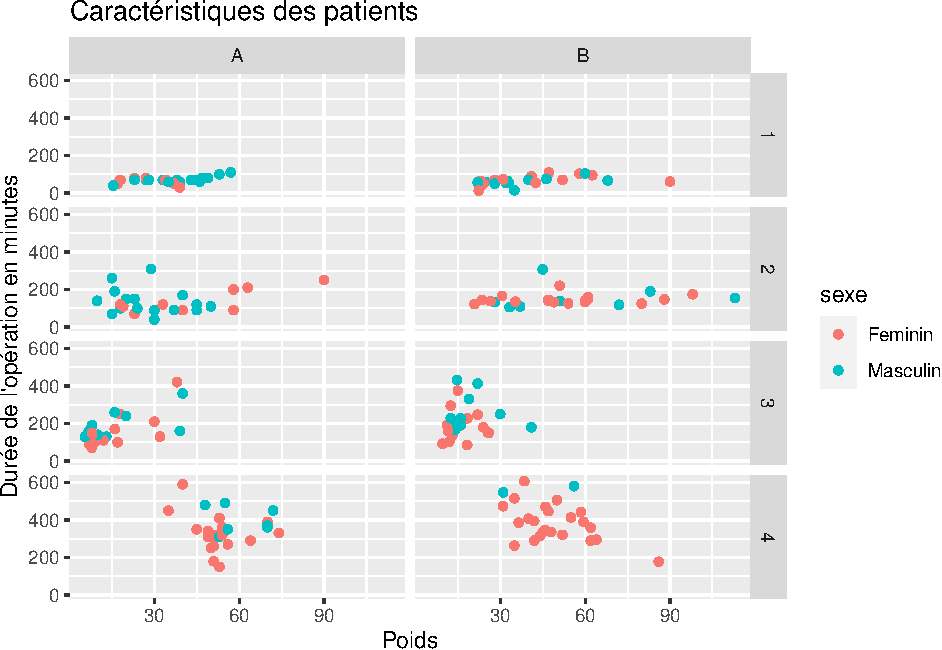
\includegraphics{_main_files/figure-latex/ggplot16-1.pdf}

Si on veut ajouter une variable de gravité inversée par rapport à la variable
CIM2, avec 1 l'opération la plus grave et 4 l'opération bénigne:

\begin{Shaded}
\begin{Highlighting}[]
\NormalTok{patient}\SpecialCharTok{$}\NormalTok{Gravité }\OtherTok{\textless{}{-}}\NormalTok{ LETTERS[}\DecValTok{5} \SpecialCharTok{{-}}\NormalTok{ patient}\SpecialCharTok{$}\NormalTok{CIM2]}
\FunctionTok{ggplot}\NormalTok{(patient,}\FunctionTok{aes}\NormalTok{(}\AttributeTok{x=}\NormalTok{poids,}\AttributeTok{y=}\NormalTok{dureeopmin))}\SpecialCharTok{+}\FunctionTok{geom\_point}\NormalTok{(}\FunctionTok{aes}\NormalTok{(}\AttributeTok{col=}\NormalTok{sexe))}\SpecialCharTok{+}
  \FunctionTok{ggtitle}\NormalTok{(}\StringTok{"Caractéristiques des patients"}\NormalTok{) }\SpecialCharTok{+} 
  \FunctionTok{xlab}\NormalTok{(}\StringTok{"Poids"}\NormalTok{) }\SpecialCharTok{+} 
  \FunctionTok{ylab}\NormalTok{(}\StringTok{"Durée de l\textquotesingle{}opération en minutes"}\NormalTok{) }\SpecialCharTok{+}
  \FunctionTok{facet\_grid}\NormalTok{(Gravité }\SpecialCharTok{\textasciitilde{}}\NormalTok{ Hopital)}
\end{Highlighting}
\end{Shaded}

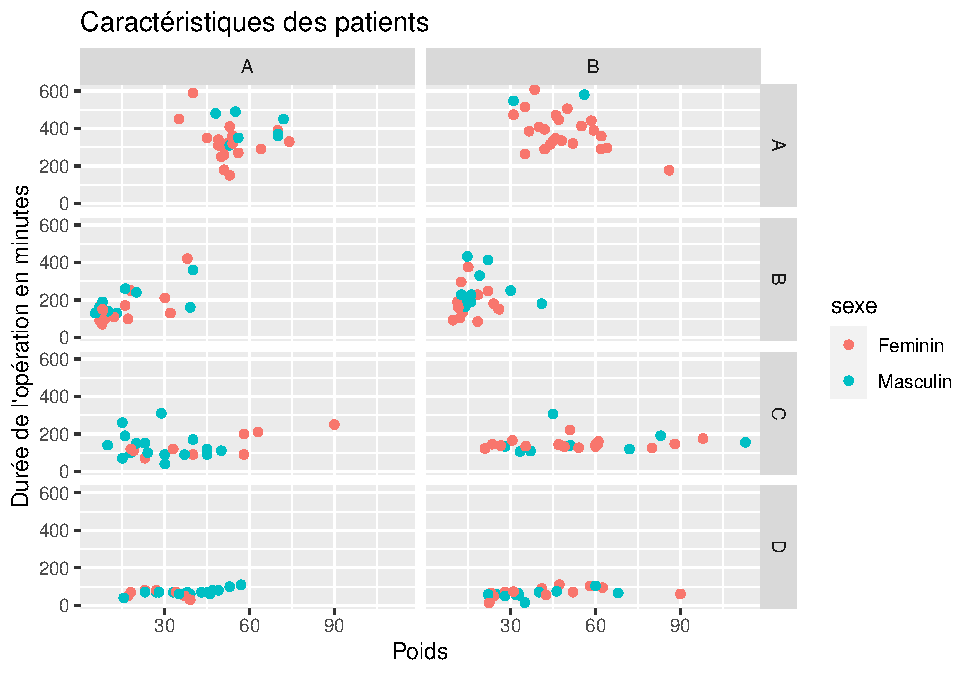
\includegraphics{_main_files/figure-latex/unnamed-chunk-77-1.pdf}

Pour rajouter une droite de régression :

\begin{Shaded}
\begin{Highlighting}[]
\FunctionTok{ggplot}\NormalTok{(patient,}\FunctionTok{aes}\NormalTok{(}\AttributeTok{x=}\NormalTok{poids,}\AttributeTok{y=}\NormalTok{dureeopmin))}\SpecialCharTok{+}\FunctionTok{geom\_point}\NormalTok{(}\FunctionTok{aes}\NormalTok{(}\AttributeTok{col=}\NormalTok{sexe))}\SpecialCharTok{+}
  \FunctionTok{geom\_smooth}\NormalTok{(}\AttributeTok{method=}\StringTok{"lm"}\NormalTok{) }\SpecialCharTok{+}
  \FunctionTok{ggtitle}\NormalTok{(}\StringTok{"Caractéristiques des patients"}\NormalTok{) }\SpecialCharTok{+} 
  \FunctionTok{xlab}\NormalTok{(}\StringTok{"Poids"}\NormalTok{) }\SpecialCharTok{+} 
  \FunctionTok{ylab}\NormalTok{(}\StringTok{"Durée de l\textquotesingle{}opération en minutes"}\NormalTok{) }\SpecialCharTok{+}
  \FunctionTok{facet\_grid}\NormalTok{(CIM2 }\SpecialCharTok{\textasciitilde{}}\NormalTok{ Hopital)}
\end{Highlighting}
\end{Shaded}

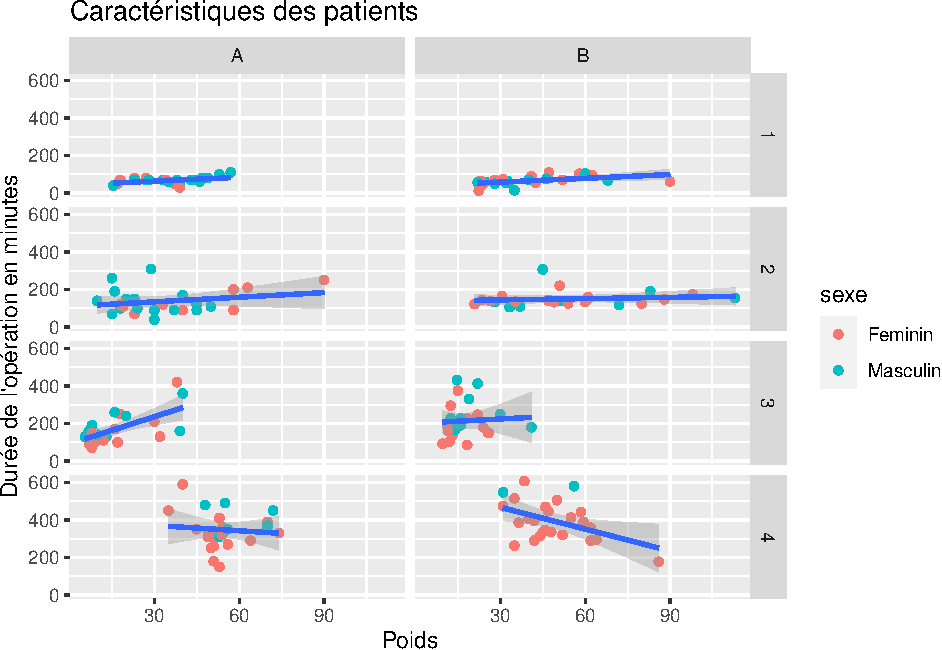
\includegraphics{_main_files/figure-latex/ggplot17a-1.pdf}
Des courbes de tendances :

\begin{Shaded}
\begin{Highlighting}[]
\FunctionTok{ggplot}\NormalTok{(patient,}\FunctionTok{aes}\NormalTok{(}\AttributeTok{x=}\NormalTok{poids,}\AttributeTok{y=}\NormalTok{dureeopmin))}\SpecialCharTok{+}\FunctionTok{geom\_point}\NormalTok{(}\FunctionTok{aes}\NormalTok{(}\AttributeTok{col=}\NormalTok{sexe))}\SpecialCharTok{+}
  \FunctionTok{geom\_smooth}\NormalTok{() }\SpecialCharTok{+}
  \FunctionTok{ggtitle}\NormalTok{(}\StringTok{"Caractéristiques des patients"}\NormalTok{) }\SpecialCharTok{+} 
  \FunctionTok{xlab}\NormalTok{(}\StringTok{"Poids"}\NormalTok{) }\SpecialCharTok{+} 
  \FunctionTok{ylab}\NormalTok{(}\StringTok{"Durée de l\textquotesingle{}opération en minutes"}\NormalTok{) }\SpecialCharTok{+}
  \FunctionTok{facet\_grid}\NormalTok{(CIM2 }\SpecialCharTok{\textasciitilde{}}\NormalTok{ Hopital)}
\end{Highlighting}
\end{Shaded}

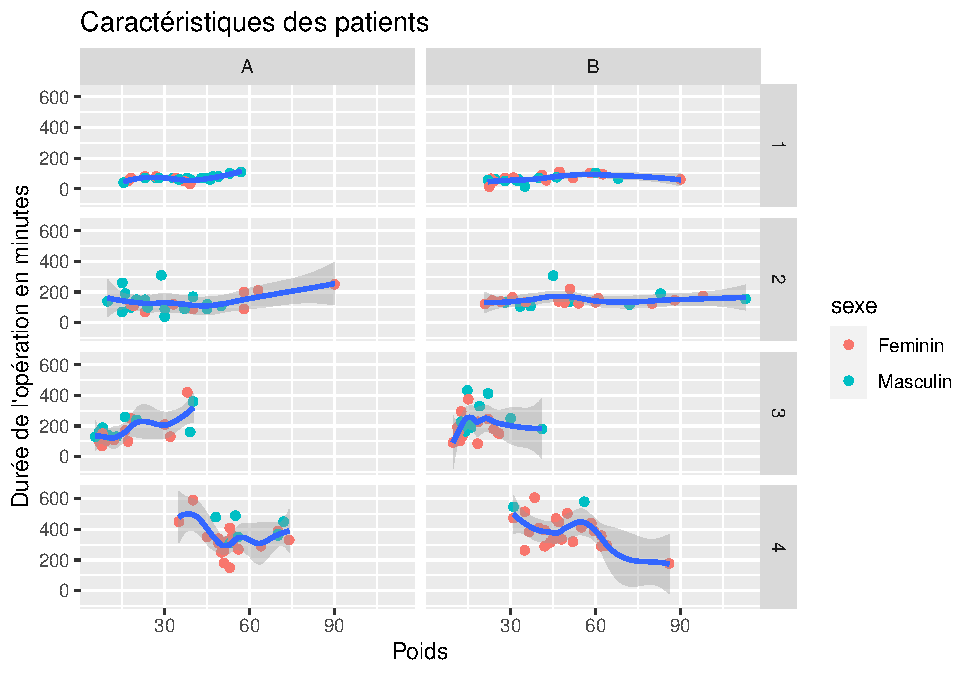
\includegraphics{_main_files/figure-latex/ggplot18-1.pdf}

Sans l'intervalle de confiance :

\begin{Shaded}
\begin{Highlighting}[]
\FunctionTok{ggplot}\NormalTok{(patient,}\FunctionTok{aes}\NormalTok{(}\AttributeTok{x=}\NormalTok{vitaux,}\AttributeTok{y=}\NormalTok{totalechelle))}\SpecialCharTok{+}\FunctionTok{geom\_point}\NormalTok{(}\FunctionTok{aes}\NormalTok{(}\AttributeTok{col=}\NormalTok{sexe))}\SpecialCharTok{+}
  \FunctionTok{geom\_smooth}\NormalTok{(}\AttributeTok{se=}\ConstantTok{FALSE}\NormalTok{) }\SpecialCharTok{+}
  \FunctionTok{ggtitle}\NormalTok{(}\StringTok{"Caractéristiques des patients"}\NormalTok{) }\SpecialCharTok{+} 
  \FunctionTok{xlab}\NormalTok{(}\StringTok{"Poids"}\NormalTok{) }\SpecialCharTok{+} 
  \FunctionTok{ylab}\NormalTok{(}\StringTok{"Durée de l\textquotesingle{}opération en minutes"}\NormalTok{) }\SpecialCharTok{+}
  \FunctionTok{facet\_grid}\NormalTok{(CIM2 }\SpecialCharTok{\textasciitilde{}}\NormalTok{ Hopital)}
\end{Highlighting}
\end{Shaded}

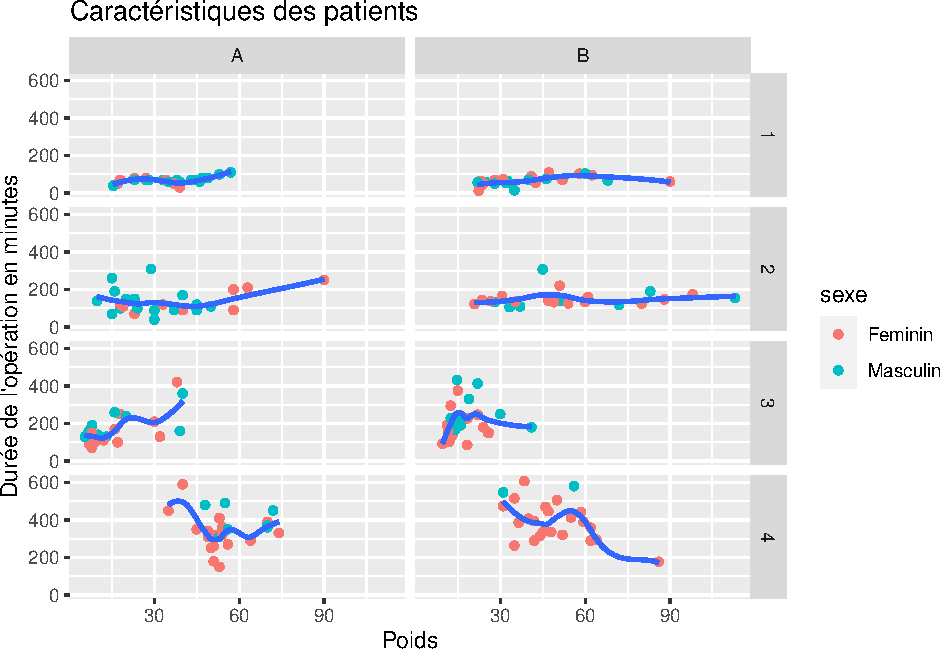
\includegraphics{_main_files/figure-latex/ggplot19-1.pdf}

Avec l'intervalle de confiance et la droite de régression :

\begin{Shaded}
\begin{Highlighting}[]
\FunctionTok{ggplot}\NormalTok{(patient,}\FunctionTok{aes}\NormalTok{(}\AttributeTok{x=}\NormalTok{dureeopmin,}\AttributeTok{y=}\NormalTok{totalechelle))}\SpecialCharTok{+}\FunctionTok{geom\_point}\NormalTok{(}\FunctionTok{aes}\NormalTok{(}\AttributeTok{col=}\NormalTok{sexe))}\SpecialCharTok{+}
  \FunctionTok{geom\_smooth}\NormalTok{(}\AttributeTok{method=}\StringTok{"lm"}\NormalTok{,}\AttributeTok{se=}\ConstantTok{FALSE}\NormalTok{) }\SpecialCharTok{+}
  \FunctionTok{ggtitle}\NormalTok{(}\StringTok{"Total des échelles de douleur et durée opération"}\NormalTok{) }\SpecialCharTok{+} 
  \FunctionTok{xlab}\NormalTok{(}\StringTok{"Durée de l\textquotesingle{}opération en minutes"}\NormalTok{) }\SpecialCharTok{+} 
  \FunctionTok{ylab}\NormalTok{(}\StringTok{"Total des échelles de douleur"}\NormalTok{) }\SpecialCharTok{+}
  \FunctionTok{facet\_grid}\NormalTok{(CIM2 }\SpecialCharTok{\textasciitilde{}}\NormalTok{ Hopital)}
\end{Highlighting}
\end{Shaded}

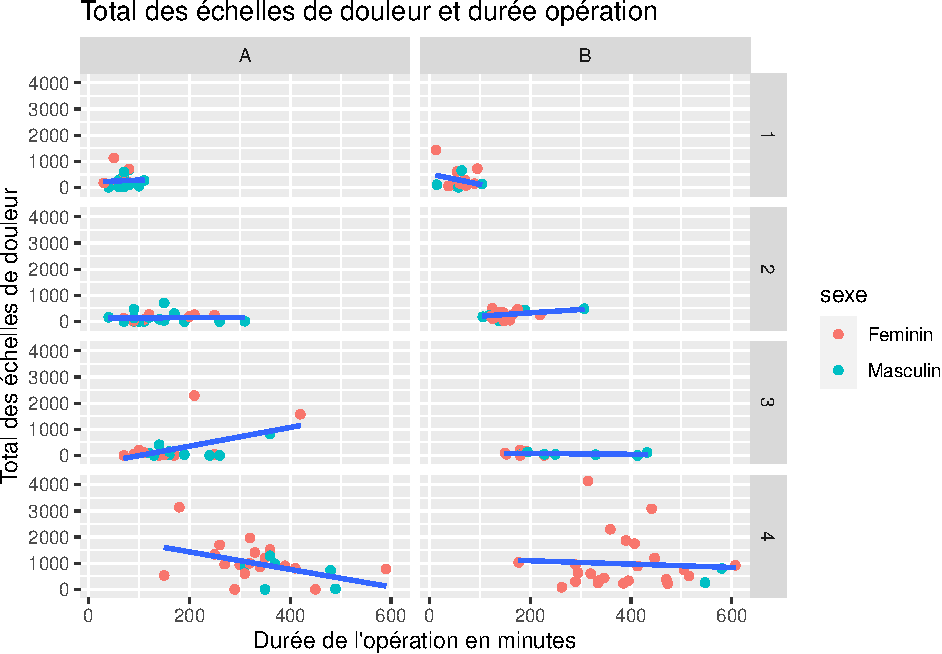
\includegraphics{_main_files/figure-latex/ggplot20-1.pdf}

Pour ajouter des étiquettes, il existe la librairie \textbf{ggrepel} qui permet
de faire en sorte que la superposition des étiquettes soit minimale :

\begin{Shaded}
\begin{Highlighting}[]
\FunctionTok{ggplot}\NormalTok{(patient,}\FunctionTok{aes}\NormalTok{(}\AttributeTok{x=}\NormalTok{dureeopmin,}\AttributeTok{y=}\NormalTok{totalechelle,}\AttributeTok{label=}\NormalTok{UID))}\SpecialCharTok{+}\FunctionTok{geom\_point}\NormalTok{(}\FunctionTok{aes}\NormalTok{(}\AttributeTok{col=}\NormalTok{sexe))}\SpecialCharTok{+}
  \FunctionTok{geom\_smooth}\NormalTok{(}\AttributeTok{method=}\StringTok{"lm"}\NormalTok{,}\AttributeTok{se=}\ConstantTok{FALSE}\NormalTok{) }\SpecialCharTok{+}
  \FunctionTok{geom\_text\_repel}\NormalTok{() }\SpecialCharTok{+}
  \FunctionTok{ggtitle}\NormalTok{(}\StringTok{"Total des échelles de douleur et durée opération"}\NormalTok{) }\SpecialCharTok{+} 
  \FunctionTok{xlab}\NormalTok{(}\StringTok{"Durée de l\textquotesingle{}opération en minutes"}\NormalTok{) }\SpecialCharTok{+} 
  \FunctionTok{ylab}\NormalTok{(}\StringTok{"Total des échelles de douleur"}\NormalTok{) }
\end{Highlighting}
\end{Shaded}

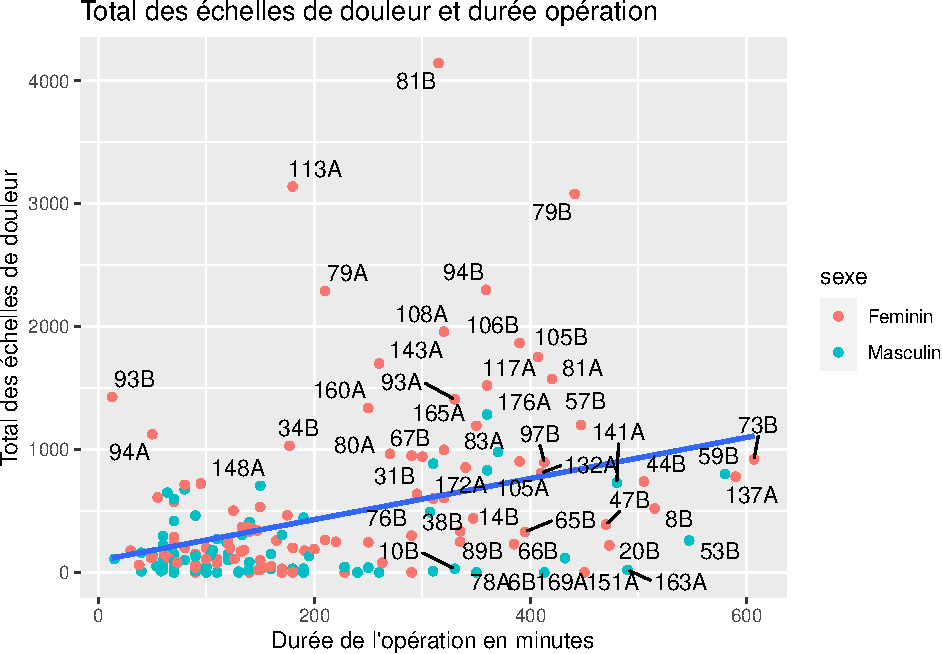
\includegraphics{_main_files/figure-latex/ggplot21-1.pdf}

Evidemment toutes les étiquettes ne sont pas dessinés car il y a trop d'individus
mais cela permet de repérer les individus atypiques.

\hypertarget{tableaux-de-contingences}{%
\subsection{Tableaux de contingences}\label{tableaux-de-contingences}}

Pour les tableaux de fréquences, on peut faire très simple :

\begin{Shaded}
\begin{Highlighting}[]
\FunctionTok{ggplot}\NormalTok{(patient,}\FunctionTok{aes}\NormalTok{(sexe))}\SpecialCharTok{+}\FunctionTok{geom\_bar}\NormalTok{()}
\end{Highlighting}
\end{Shaded}

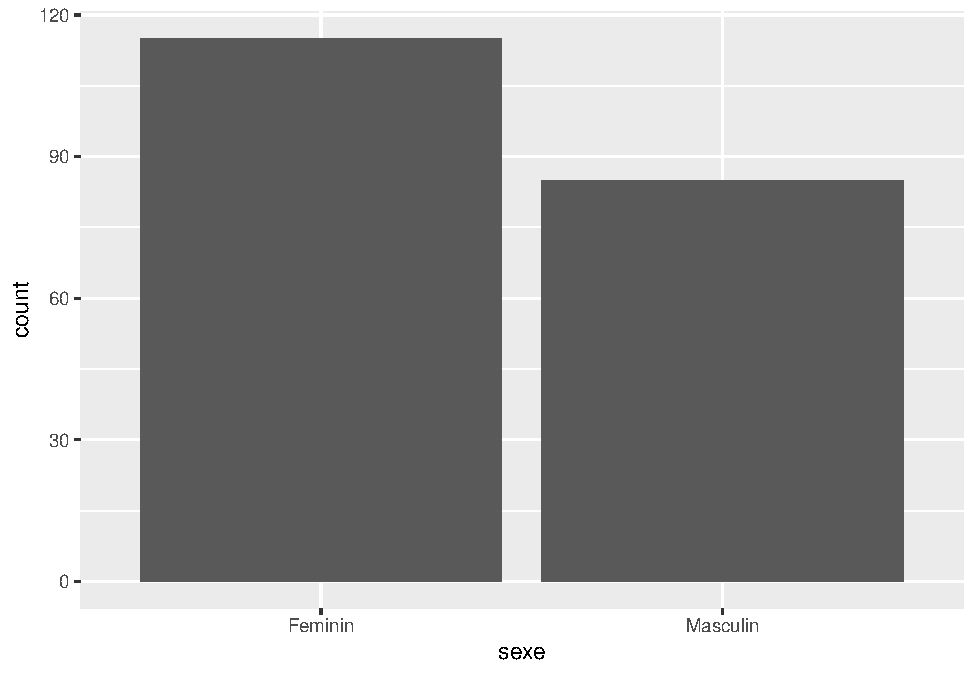
\includegraphics{_main_files/figure-latex/ggplot17b-1.pdf}

\begin{Shaded}
\begin{Highlighting}[]
\FunctionTok{ggplot}\NormalTok{(patient,}\FunctionTok{aes}\NormalTok{(sexe))}\SpecialCharTok{+}\FunctionTok{geom\_bar}\NormalTok{()}\SpecialCharTok{+}
  \FunctionTok{facet\_grid}\NormalTok{(.}\SpecialCharTok{\textasciitilde{}}\NormalTok{Hopital)}
\end{Highlighting}
\end{Shaded}

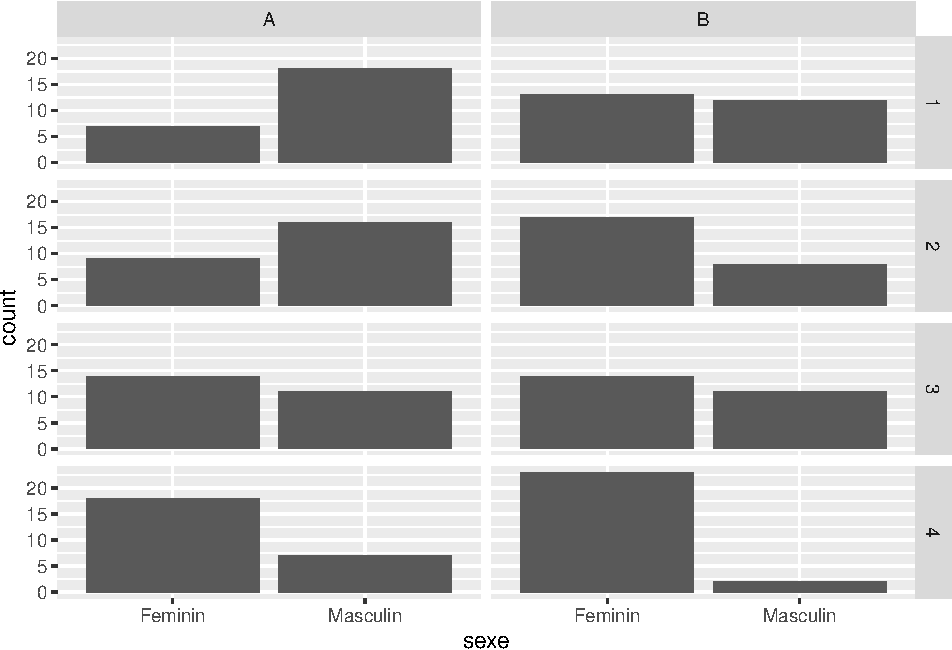
\includegraphics{_main_files/figure-latex/ggplot18b-1.pdf}
Là où \textbf{ggplot2} commence à devenir compliqué, c'est que \textbf{geom\_bar} ne va pas
marcher car il faut lui fournir la \textbf{data.frame} avec les statistiques \textbf{en ligne}.

Soit :

\begin{verbatim}
##       sexe CIM2 effectif
## 1  Feminin    1       20
## 2 Masculin    1       30
## 3  Feminin    2       26
## 4 Masculin    2       24
## 5  Feminin    3       28
## 6 Masculin    3       22
## 7  Feminin    4       41
## 8 Masculin    4        9
\end{verbatim}

Pour faire ce tableau, il faut faire appel au \textbf{package} \textbf{reshape2}.

\begin{Shaded}
\begin{Highlighting}[]
\FunctionTok{require}\NormalTok{(reshape2)}
\NormalTok{tableau }\OtherTok{\textless{}{-}} \FunctionTok{table}\NormalTok{(patient}\SpecialCharTok{$}\NormalTok{sexe,patient}\SpecialCharTok{$}\NormalTok{CIM2)}
\NormalTok{tableau}
\end{Highlighting}
\end{Shaded}

\begin{verbatim}
##           
##             1  2  3  4
##   Feminin  20 26 28 41
##   Masculin 30 24 22  9
\end{verbatim}

De ce tableau on passe au long en une commande :

\begin{Shaded}
\begin{Highlighting}[]
\NormalTok{long }\OtherTok{\textless{}{-}} \FunctionTok{melt}\NormalTok{(tableau,}\AttributeTok{varnames =} \FunctionTok{c}\NormalTok{(}\StringTok{"sexe"}\NormalTok{,}\StringTok{"CIM2"}\NormalTok{),}\AttributeTok{value.name =} \StringTok{"value"}\NormalTok{)}
\end{Highlighting}
\end{Shaded}

Il faut spécifier le nom à donner aux deux variables et spécifier le résultat
du croisement des deux variables qui est le nombre d'observations c'est-à-dire
le contenu de chaque cellule de \textbf{tableau}.

\begin{Shaded}
\begin{Highlighting}[]
\FunctionTok{ggplot}\NormalTok{(long,}\FunctionTok{aes}\NormalTok{(}\AttributeTok{x=}\NormalTok{sexe,}\AttributeTok{y=}\NormalTok{value,}\AttributeTok{fill=}\NormalTok{CIM2))}\SpecialCharTok{+}\FunctionTok{geom\_bar}\NormalTok{(}\AttributeTok{position =} \StringTok{"stack"}\NormalTok{,}\AttributeTok{stat=}\StringTok{"identity"}\NormalTok{)}
\end{Highlighting}
\end{Shaded}

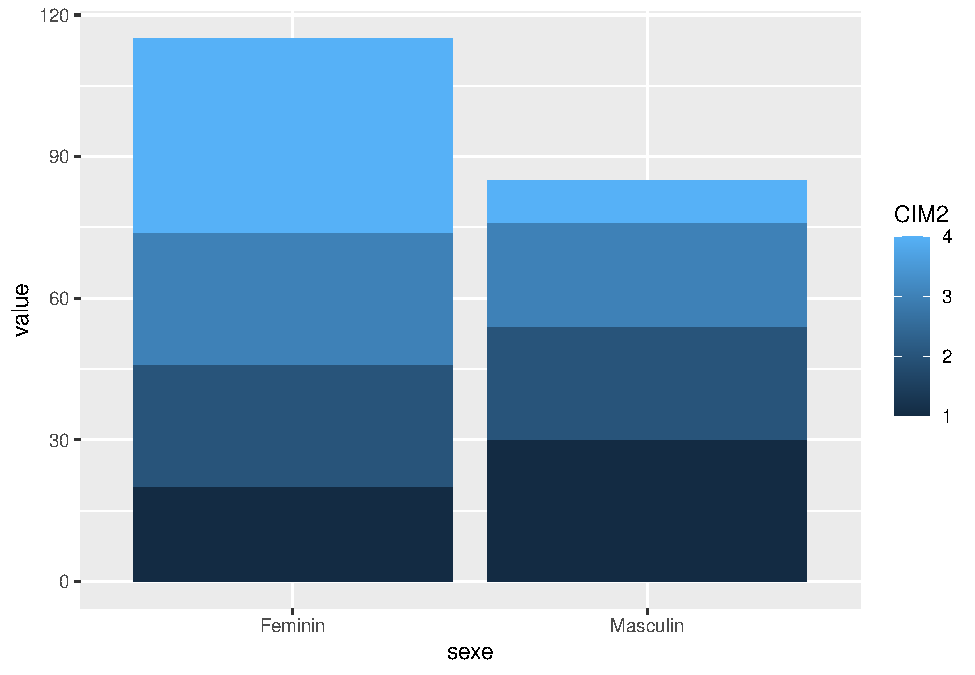
\includegraphics{_main_files/figure-latex/ggplot30-1.pdf}

Je dois faire de CIM2 une variable qualitative explicitement. En effet, CIM2 est numérique
(un entier de 1 à 4). Aussi quand je donne le CIM2 à l'argument \textbf{fill=} il ne sait pas
s'il s'agit de la couleur (qui peut être un code numérique aussi) ou d'une variable qualitative.

\begin{Shaded}
\begin{Highlighting}[]
\FunctionTok{ggplot}\NormalTok{(long,}\FunctionTok{aes}\NormalTok{(}\AttributeTok{x=}\NormalTok{sexe,}\AttributeTok{y=}\NormalTok{value,}\AttributeTok{fill=}\FunctionTok{factor}\NormalTok{(CIM2)))}\SpecialCharTok{+}\FunctionTok{geom\_bar}\NormalTok{(}\AttributeTok{position =} \StringTok{"dodge"}\NormalTok{,}\AttributeTok{stat=}\StringTok{"identity"}\NormalTok{)}
\end{Highlighting}
\end{Shaded}

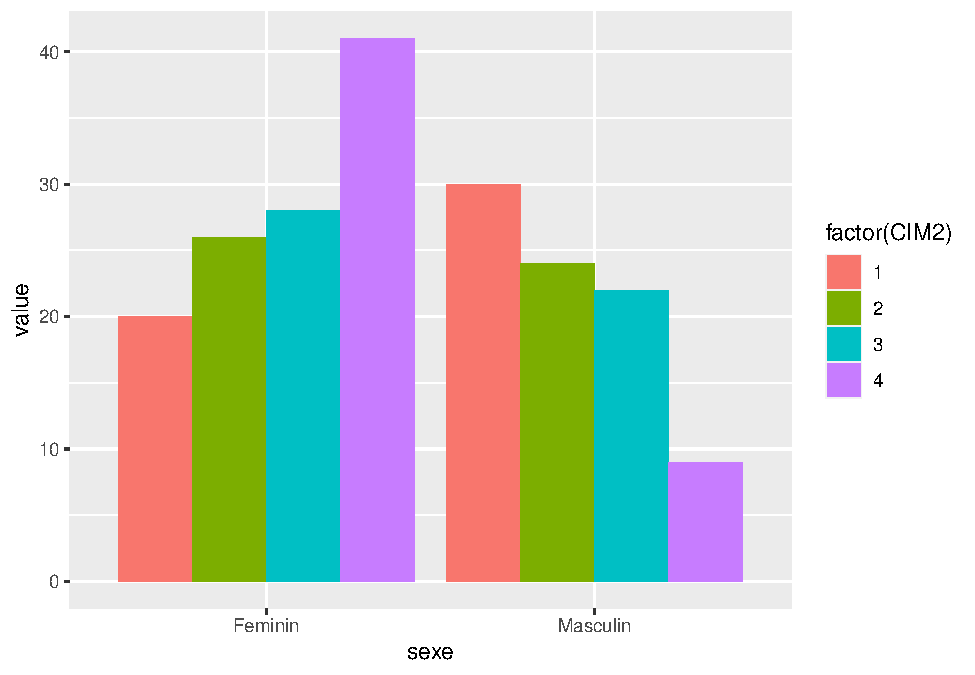
\includegraphics{_main_files/figure-latex/ggplot31-1.pdf}

D'où le graphique :

\begin{Shaded}
\begin{Highlighting}[]
\NormalTok{tableau }\OtherTok{\textless{}{-}} \FunctionTok{table}\NormalTok{(patient}\SpecialCharTok{$}\NormalTok{Hopital,patient}\SpecialCharTok{$}\NormalTok{sexe,patient}\SpecialCharTok{$}\NormalTok{CIM2)}
\NormalTok{long }\OtherTok{\textless{}{-}} \FunctionTok{melt}\NormalTok{(tableau,}\AttributeTok{varnames =} \FunctionTok{c}\NormalTok{(}\StringTok{"Hopital"}\NormalTok{,}\StringTok{"sexe"}\NormalTok{,}\StringTok{"CIM2"}\NormalTok{),}\AttributeTok{value.name =} \StringTok{"effectif"}\NormalTok{)}
\FunctionTok{ggplot}\NormalTok{(long,}\FunctionTok{aes}\NormalTok{(}\AttributeTok{x=}\NormalTok{CIM2,}\AttributeTok{y=}\NormalTok{effectif,}\AttributeTok{fill=}\NormalTok{sexe))}\SpecialCharTok{+}
  \FunctionTok{geom\_bar}\NormalTok{(}\AttributeTok{position =} \StringTok{"dodge"}\NormalTok{,}\AttributeTok{stat=}\StringTok{"identity"}\NormalTok{)}\SpecialCharTok{+}
  \FunctionTok{facet\_grid}\NormalTok{(Hopital }\SpecialCharTok{\textasciitilde{}}\NormalTok{ . )}
\end{Highlighting}
\end{Shaded}

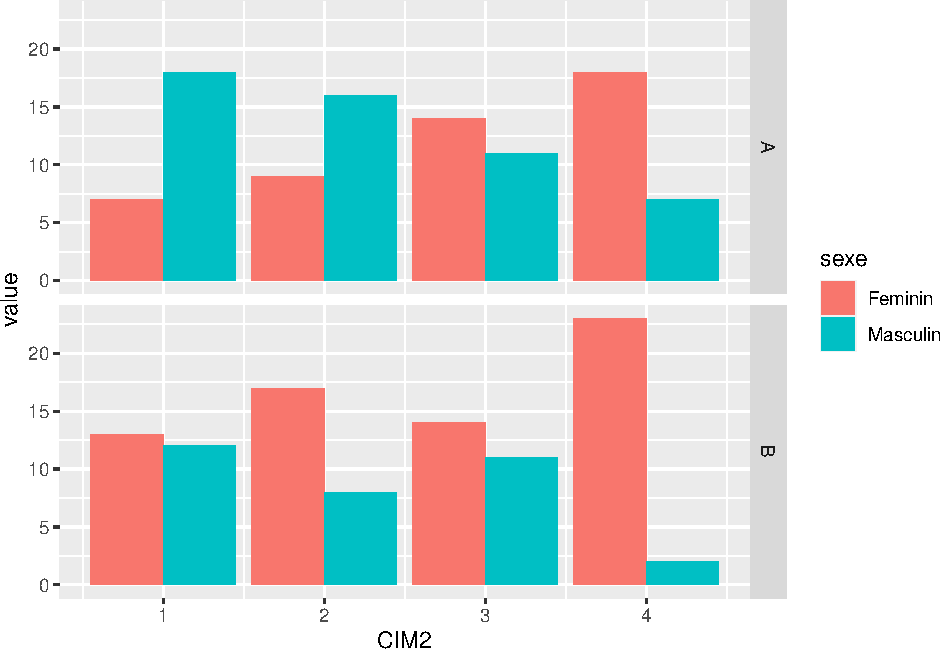
\includegraphics{_main_files/figure-latex/ggplot32-1.pdf}

Pour sauvegarder un graphique \textbf{ggplot2}, la syntaxe est différente et surtout
on l'appelle une fois que le graphique est terminé, c'est-à-dire en dernier :

Et ainsi de suite\ldots{}

\hypertarget{les-thuxe8mes}{%
\subsection{Les thèmes}\label{les-thuxe8mes}}

Les graphiques de ggplot peuvent changer selon des thèmes qui définissent des styles
de graphique différents. Celui à retenir est minimal qui fait que le graphique
est épuré au maximum :

\begin{Shaded}
\begin{Highlighting}[]
\NormalTok{tableau }\OtherTok{\textless{}{-}} \FunctionTok{table}\NormalTok{(patient}\SpecialCharTok{$}\NormalTok{Hopital,patient}\SpecialCharTok{$}\NormalTok{sexe,patient}\SpecialCharTok{$}\NormalTok{CIM2)}
\NormalTok{long }\OtherTok{\textless{}{-}} \FunctionTok{melt}\NormalTok{(tableau,}\AttributeTok{varnames =} \FunctionTok{c}\NormalTok{(}\StringTok{"Hopital"}\NormalTok{,}\StringTok{"sexe"}\NormalTok{,}\StringTok{"CIM2"}\NormalTok{),}\AttributeTok{value.name =} \StringTok{"effectif"}\NormalTok{)}
\FunctionTok{ggplot}\NormalTok{(long,}\FunctionTok{aes}\NormalTok{(}\AttributeTok{x=}\NormalTok{CIM2,}\AttributeTok{y=}\NormalTok{effectif,}\AttributeTok{fill=}\NormalTok{sexe))}\SpecialCharTok{+}
  \FunctionTok{geom\_bar}\NormalTok{(}\AttributeTok{position =} \StringTok{"dodge"}\NormalTok{,}\AttributeTok{stat=}\StringTok{"identity"}\NormalTok{)}\SpecialCharTok{+}
  \FunctionTok{facet\_grid}\NormalTok{(Hopital }\SpecialCharTok{\textasciitilde{}}\NormalTok{ . ) }\SpecialCharTok{+} \FunctionTok{theme\_minimal}\NormalTok{()}
\end{Highlighting}
\end{Shaded}

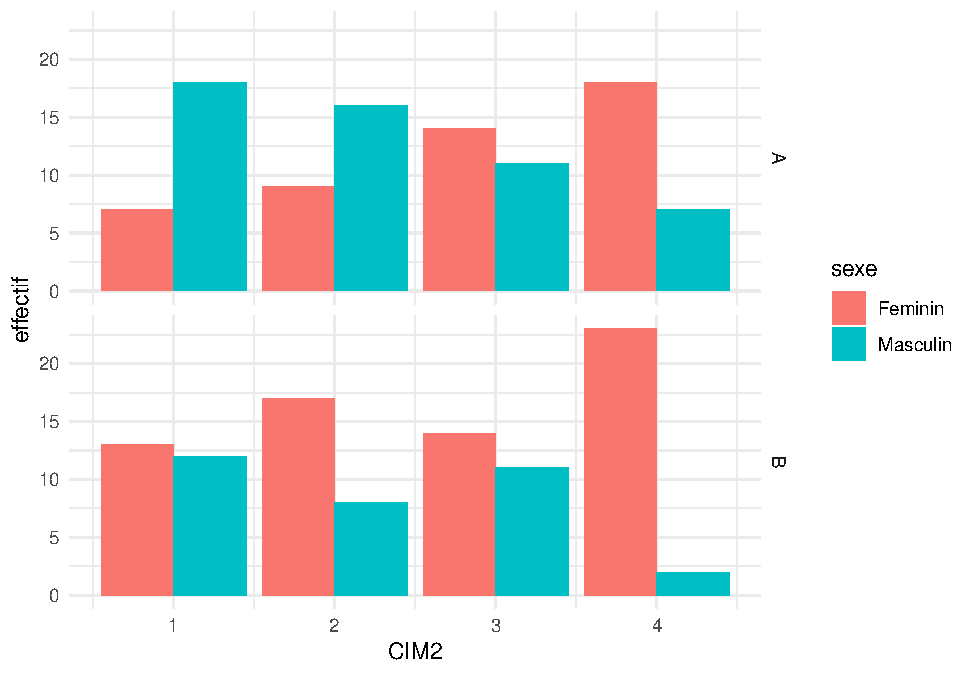
\includegraphics{_main_files/figure-latex/unnamed-chunk-82-1.pdf}

Il y a 10 à 20 thèmes par défaut et il y a des variantes supplémentaires et de
quoi personnaliser ses propres thèmes dans le package \textbf{ggthemes}.

\hypertarget{liens}{%
\section{Liens}\label{liens}}

Il y a de nombreuses galleries sur le web avec toutes les possiblités offertes
par les graphiques de base comme les graphiques avec \textbf{ggplot2}.

\begin{itemize}
\tightlist
\item
  \href{https://r-graph-gallery.com/}{r-graph-gallery}
\item
  \href{https://r-charts.com/ggplot2/}{r-chart}
\item
  \ldots{}
\end{itemize}

On peut en parcourir ensemble\ldots{}

\begin{Shaded}
\begin{Highlighting}[]
\NormalTok{tableau }\OtherTok{\textless{}{-}} \FunctionTok{dcast}\NormalTok{(patient, UID }\SpecialCharTok{+}\NormalTok{ sexe }\SpecialCharTok{\textasciitilde{}}\NormalTok{ Hopital, }\AttributeTok{value.var =} \StringTok{"nbechelle"}\NormalTok{)}
\NormalTok{tableau}\SpecialCharTok{$}\NormalTok{poids }\OtherTok{\textless{}{-}} \FunctionTok{ifelse}\NormalTok{(}\SpecialCharTok{!}\FunctionTok{is.na}\NormalTok{(tableau}\SpecialCharTok{$}\NormalTok{A),tableau}\SpecialCharTok{$}\NormalTok{A,tableau}\SpecialCharTok{$}\NormalTok{B)}

\FunctionTok{ggplot}\NormalTok{(tableau, }\FunctionTok{aes}\NormalTok{(}\AttributeTok{x=}\NormalTok{nbechelle) ) }\SpecialCharTok{+}
  \FunctionTok{geom\_density}\NormalTok{( }\FunctionTok{aes}\NormalTok{(}\AttributeTok{x =}\NormalTok{ A, }\AttributeTok{y =}\NormalTok{ ..density..), }\AttributeTok{fill=}\StringTok{"\#69b3a2"}\NormalTok{ ) }\SpecialCharTok{+}
  \FunctionTok{geom\_label}\NormalTok{(}\FunctionTok{aes}\NormalTok{(}\AttributeTok{x=}\DecValTok{90}\NormalTok{, }\AttributeTok{y=}\FloatTok{0.01}\NormalTok{, }\AttributeTok{label=}\StringTok{"Hopital A"}\NormalTok{), }\AttributeTok{color=}\StringTok{"\#69b3a2"}\NormalTok{) }\SpecialCharTok{+}
  \FunctionTok{geom\_density}\NormalTok{( }\FunctionTok{aes}\NormalTok{(}\AttributeTok{x =}\NormalTok{ B, }\AttributeTok{y =} \SpecialCharTok{{-}}\NormalTok{..density..), }\AttributeTok{fill=} \StringTok{"\#404080"}\NormalTok{) }\SpecialCharTok{+}
  \FunctionTok{geom\_label}\NormalTok{(}\FunctionTok{aes}\NormalTok{(}\AttributeTok{x=}\DecValTok{90}\NormalTok{,}\AttributeTok{y=}\SpecialCharTok{{-}}\FloatTok{0.01}\NormalTok{, }\AttributeTok{label=}\StringTok{"Hopital B"}\NormalTok{), }\AttributeTok{color=}\StringTok{"\#404080"}\NormalTok{)}
\end{Highlighting}
\end{Shaded}

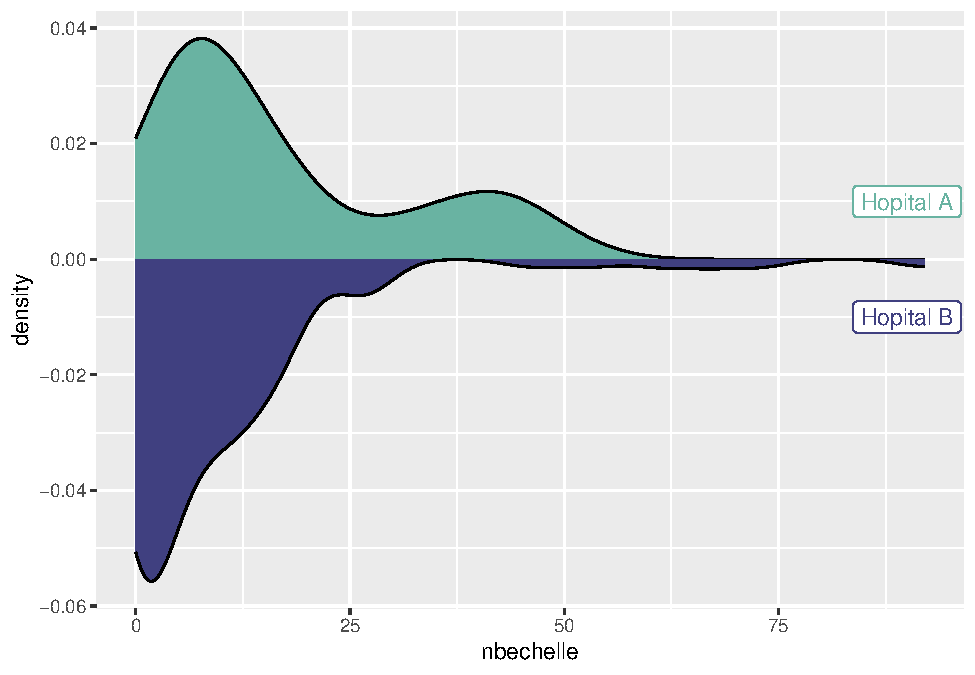
\includegraphics{_main_files/figure-latex/unnamed-chunk-83-1.pdf}

\hypertarget{manipulation-avancuxe9e-mettre-en-forme-vos-donnuxe9es}{%
\chapter{Manipulation avancée (mettre en forme vos données)}\label{manipulation-avancuxe9e-mettre-en-forme-vos-donnuxe9es}}

Le but de cette partie qui ne sera pas très longue sur le papier mais beaucoup
plus à l'apprentissage est de vous montrer comment automatiser les choses.

Pour prendre un exemple qui nous est familier, transformer en facteur ou en
variable ordinale des items de plusieurs échelles. Sous SPSS ou sous R, c'est
pénible si vous n'utilisez pas les macros pour SPSS ou la programmation
sous R.

On peut automatiser beaucoup de choses sous R. Il y a des paquets sous
R qui permettent d'analyser des modèles structuraux ou faire des pages web
interactives. Sans aller jusque là, on peut se rendre la vie plus facile.

\hypertarget{transformation-de-plusieurs-variables}{%
\section{Transformation de plusieurs variables}\label{transformation-de-plusieurs-variables}}

On va charger le \href{https://personality-project.org/r/psych/HowTo/scoring.tutorial/small.msq.txt}{fichier de données} en ligne :

\begin{Shaded}
\begin{Highlighting}[]
\NormalTok{file.name }\OtherTok{\textless{}{-}} \StringTok{"https://personality{-}project.org/r/psych/HowTo/scoring.tutorial/small.msq.txt"}
\NormalTok{msq }\OtherTok{\textless{}{-}} \FunctionTok{read\_table}\NormalTok{(file.name)}
\end{Highlighting}
\end{Shaded}

\begin{verbatim}
## 
## -- Column specification -------------------------------------------------------------------------------------------------
## cols(
##   `"active"` = col_double(),
##   `"alert"` = col_double(),
##   `"aroused"` = col_double(),
##   `"sleepy"` = col_double(),
##   `"tired"` = col_double(),
##   `"drowsy"` = col_double(),
##   `"anxious"` = col_double(),
##   `"jittery"` = col_double(),
##   `"nervous"` = col_double(),
##   `"calm"` = col_double(),
##   `"relaxed"` = col_double(),
##   `"at.ease"` = col_double(),
##   `"gender"` = col_double(),
##   `"drug"` = col_double()
## )
\end{verbatim}

Oui au passage on peut lire des fichiers de données directement en ligne.

Dans ce cas, on a utilisé la commande \textbf{read\_table} du \textbf{package readr}, car
le séparateur de champs est l'espace.

\begin{Shaded}
\begin{Highlighting}[]
\FunctionTok{str}\NormalTok{(msq)}
\end{Highlighting}
\end{Shaded}

\begin{verbatim}
## spc_tbl_ [200 x 14] (S3: spec_tbl_df/tbl_df/tbl/data.frame)
##  $ "active" : num [1:200] 2 1 1 1 1 3 1 0 3 1 ...
##  $ "alert"  : num [1:200] 2 1 1 2 2 3 1 1 3 1 ...
##  $ "aroused": num [1:200] 0 0 1 0 1 2 0 0 3 0 ...
##  $ "sleepy" : num [1:200] 0 2 3 1 1 0 2 1 0 1 ...
##  $ "tired"  : num [1:200] 1 2 3 1 1 0 2 1 0 1 ...
##  $ "drowsy" : num [1:200] 1 2 2 0 0 0 3 1 0 1 ...
##  $ "anxious": num [1:200] 1 1 2 0 0 1 0 0 3 0 ...
##  $ "jittery": num [1:200] 1 0 0 0 1 0 0 0 3 0 ...
##  $ "nervous": num [1:200] 0 1 1 0 0 0 0 0 1 0 ...
##  $ "calm"   : num [1:200] 2 2 2 2 3 2 1 3 0 1 ...
##  $ "relaxed": num [1:200] 2 2 2 2 2 3 2 2 0 2 ...
##  $ "at.ease": num [1:200] 2 2 2 2 3 3 1 2 0 2 ...
##  $ "gender" : num [1:200] 2 2 1 2 1 1 2 2 1 1 ...
##  $ "drug"   : num [1:200] 2 1 1 2 1 2 2 1 2 1 ...
##  - attr(*, "spec")=
##   .. cols(
##   ..   `"active"` = col_double(),
##   ..   `"alert"` = col_double(),
##   ..   `"aroused"` = col_double(),
##   ..   `"sleepy"` = col_double(),
##   ..   `"tired"` = col_double(),
##   ..   `"drowsy"` = col_double(),
##   ..   `"anxious"` = col_double(),
##   ..   `"jittery"` = col_double(),
##   ..   `"nervous"` = col_double(),
##   ..   `"calm"` = col_double(),
##   ..   `"relaxed"` = col_double(),
##   ..   `"at.ease"` = col_double(),
##   ..   `"gender"` = col_double(),
##   ..   `"drug"` = col_double()
##   .. )
\end{verbatim}

On voit que les guillemets ont été importés et parasite la ligne des noms de colonnes.
Pour ça on utilise \textbf{gsub}, une fonction qui remplace les caractéères dans le premier
argument par les caractères dans le deuxième. Le troisième argument est \textbf{vecteur}
dans lequel on veut remplacer le texte.

Ici on va remplacer un guillemet double, partout, par aucun caractère. Et on applique
ça aux noms de variables de msq, ce qui nous donne :

\begin{Shaded}
\begin{Highlighting}[]
\FunctionTok{colnames}\NormalTok{(msq) }\OtherTok{\textless{}{-}} \FunctionTok{gsub}\NormalTok{(}\StringTok{\textquotesingle{}"\textquotesingle{}}\NormalTok{,}\StringTok{\textquotesingle{}\textquotesingle{}}\NormalTok{,}\FunctionTok{colnames}\NormalTok{(msq),}\AttributeTok{fixed=}\NormalTok{T)}
\NormalTok{msq}
\end{Highlighting}
\end{Shaded}

\begin{verbatim}
## # A tibble: 200 x 14
##    active alert aroused sleepy tired drowsy anxious jittery nervous  calm relaxed at.ease gender  drug
##     <dbl> <dbl>   <dbl>  <dbl> <dbl>  <dbl>   <dbl>   <dbl>   <dbl> <dbl>   <dbl>   <dbl>  <dbl> <dbl>
##  1      2     2       0      0     1      1       1       1       0     2       2       2      2     2
##  2      1     1       0      2     2      2       1       0       1     2       2       2      2     1
##  3      1     1       1      3     3      2       2       0       1     2       2       2      1     1
##  4      1     2       0      1     1      0       0       0       0     2       2       2      2     2
##  5      1     2       1      1     1      0       0       1       0     3       2       3      1     1
##  6      3     3       2      0     0      0       1       0       0     2       3       3      1     2
##  7      1     1       0      2     2      3       0       0       0     1       2       1      2     2
##  8      0     1       0      1     1      1       0       0       0     3       2       2      2     1
##  9      3     3       3      0     0      0       3       3       1     0       0       0      1     2
## 10      1     1       0      1     1      1       0       0       0     1       2       2      1     1
## # i 190 more rows
\end{verbatim}

Les commentaires de read.table indique que les colonnes sont toutes des nombres
réels de double précision. C'est très bien pour les analyses psychométriques
primaires avec \textbf{psych} mais pas avec lavaan qui réclame des facteurs.

On va utiliser la machine à automatiser \textbf{mutate\_at} qui permet d'appliquer une
transformation sur une série de variable.

Dans le premier argument, on mets \textbf{vars()} et à l'intérieur quelque chose pour
définir une ou des variables comme avec un \textbf{select}.

Le deuxième argument est la fonction à appliquer et après les arguments optionnels.

\begin{Shaded}
\begin{Highlighting}[]
\NormalTok{msq\_fact }\OtherTok{\textless{}{-}}\NormalTok{ msq}
\NormalTok{msq\_fact }\OtherTok{\textless{}{-}}\NormalTok{ msq\_fact }\SpecialCharTok{\%\textgreater{}\%} \FunctionTok{mutate}\NormalTok{(}\FunctionTok{across}\NormalTok{(active}\SpecialCharTok{:}\NormalTok{at.ease,}\SpecialCharTok{\textasciitilde{}} \FunctionTok{factor}\NormalTok{(.x,}\AttributeTok{ordered=}\NormalTok{T)))}
\end{Highlighting}
\end{Shaded}

Pour être vraiment propre, on spécifierait les niveaux :

\begin{Shaded}
\begin{Highlighting}[]
\NormalTok{msq\_fact }\OtherTok{\textless{}{-}}\NormalTok{ msq\_fact }\SpecialCharTok{\%\textgreater{}\%} \FunctionTok{mutate}\NormalTok{(}\FunctionTok{across}\NormalTok{(active}\SpecialCharTok{:}\NormalTok{at.ease, }\SpecialCharTok{\textasciitilde{}} \FunctionTok{factor}\NormalTok{(.x,}\AttributeTok{levels=}\FunctionTok{c}\NormalTok{(}\DecValTok{0}\NormalTok{,}\DecValTok{1}\NormalTok{,}\DecValTok{2}\NormalTok{,}\DecValTok{3}\NormalTok{),}\AttributeTok{ordered=}\NormalTok{T)))}
\end{Highlighting}
\end{Shaded}

\begin{Shaded}
\begin{Highlighting}[]
\FunctionTok{str}\NormalTok{(msq\_fact)}
\end{Highlighting}
\end{Shaded}

\begin{verbatim}
## tibble [200 x 14] (S3: tbl_df/tbl/data.frame)
##  $ active : Ord.factor w/ 4 levels "0"<"1"<"2"<"3": 3 2 2 2 2 4 2 1 4 2 ...
##  $ alert  : Ord.factor w/ 4 levels "0"<"1"<"2"<"3": 3 2 2 3 3 4 2 2 4 2 ...
##  $ aroused: Ord.factor w/ 4 levels "0"<"1"<"2"<"3": 1 1 2 1 2 3 1 1 4 1 ...
##  $ sleepy : Ord.factor w/ 4 levels "0"<"1"<"2"<"3": 1 3 4 2 2 1 3 2 1 2 ...
##  $ tired  : Ord.factor w/ 4 levels "0"<"1"<"2"<"3": 2 3 4 2 2 1 3 2 1 2 ...
##  $ drowsy : Ord.factor w/ 4 levels "0"<"1"<"2"<"3": 2 3 3 1 1 1 4 2 1 2 ...
##  $ anxious: Ord.factor w/ 4 levels "0"<"1"<"2"<"3": 2 2 3 1 1 2 1 1 4 1 ...
##  $ jittery: Ord.factor w/ 4 levels "0"<"1"<"2"<"3": 2 1 1 1 2 1 1 1 4 1 ...
##  $ nervous: Ord.factor w/ 4 levels "0"<"1"<"2"<"3": 1 2 2 1 1 1 1 1 2 1 ...
##  $ calm   : Ord.factor w/ 4 levels "0"<"1"<"2"<"3": 3 3 3 3 4 3 2 4 1 2 ...
##  $ relaxed: Ord.factor w/ 4 levels "0"<"1"<"2"<"3": 3 3 3 3 3 4 3 3 1 3 ...
##  $ at.ease: Ord.factor w/ 4 levels "0"<"1"<"2"<"3": 3 3 3 3 4 4 2 3 1 3 ...
##  $ gender : num [1:200] 2 2 1 2 1 1 2 2 1 1 ...
##  $ drug   : num [1:200] 2 1 1 2 1 2 2 1 2 1 ...
\end{verbatim}

Il y a des variantes à \textbf{mutate\_at} comme \textbf{mutate\_if}.

Par exemple, pour centrer/réduire les variables numériques :

\begin{Shaded}
\begin{Highlighting}[]
\NormalTok{iris }\OtherTok{\textless{}{-}}\NormalTok{ iris }\SpecialCharTok{\%\textgreater{}\%} \FunctionTok{mutate}\NormalTok{(}\FunctionTok{across}\NormalTok{(}\FunctionTok{where}\NormalTok{(is.numeric),scale))}
\end{Highlighting}
\end{Shaded}

Si la variable est numérique alors R va centrer/réduire la variable. Donc pas
de problème avec \textbf{Species} qui est un facteur :

\begin{Shaded}
\begin{Highlighting}[]
\FunctionTok{str}\NormalTok{(iris)}
\end{Highlighting}
\end{Shaded}

\begin{verbatim}
## 'data.frame':    150 obs. of  5 variables:
##  $ Sepal.Length: num [1:150, 1] -0.898 -1.139 -1.381 -1.501 -1.018 ...
##   ..- attr(*, "scaled:center")= num 5.84
##   ..- attr(*, "scaled:scale")= num 0.828
##  $ Sepal.Width : num [1:150, 1] 1.0156 -0.1315 0.3273 0.0979 1.245 ...
##   ..- attr(*, "scaled:center")= num 3.06
##   ..- attr(*, "scaled:scale")= num 0.436
##  $ Petal.Length: num [1:150, 1] -1.34 -1.34 -1.39 -1.28 -1.34 ...
##   ..- attr(*, "scaled:center")= num 3.76
##   ..- attr(*, "scaled:scale")= num 1.77
##  $ Petal.Width : num [1:150, 1] -1.31 -1.31 -1.31 -1.31 -1.31 ...
##   ..- attr(*, "scaled:center")= num 1.2
##   ..- attr(*, "scaled:scale")= num 0.762
##  $ Species     : Factor w/ 3 levels "setosa","versicolor",..: 1 1 1 1 1 1 1 1 1 1 ...
\end{verbatim}

Soit :

\begin{Shaded}
\begin{Highlighting}[]
\NormalTok{iris }\SpecialCharTok{\%\textgreater{}\%} \FunctionTok{tbl\_summary}\NormalTok{(}\AttributeTok{statistic =} \FunctionTok{list}\NormalTok{(}
  \FunctionTok{all\_continuous}\NormalTok{() }\SpecialCharTok{\textasciitilde{}} \StringTok{"\{mean\} (\{sd\})"}\NormalTok{),}\AttributeTok{type =} \FunctionTok{c}\NormalTok{(Sepal.Length}\SpecialCharTok{:}\NormalTok{Petal.Width) }\SpecialCharTok{\textasciitilde{}} \StringTok{"continuous"}\NormalTok{)}
\end{Highlighting}
\end{Shaded}

\begin{tabular}{l|c}
\hline
**Caractéristique** & **N = 150**\\
\hline
Sepal.Length & 0,00 (1,00)\\
\hline
Sepal.Width & 0,00 (1,00)\\
\hline
Petal.Length & 0,00 (1,00)\\
\hline
Petal.Width & 0,00 (1,00)\\
\hline
Species & \\
\hline
setosa & 50 (33\%)\\
\hline
versicolor & 50 (33\%)\\
\hline
virginica & 50 (33\%)\\
\hline
\end{tabular}

\hypertarget{opuxe9rateurs-et-case_when}{%
\section{Opérateurs et case\_when}\label{opuxe9rateurs-et-case_when}}

On appelle opérateur des mots-clefs généralement symbolique comme les +,/,==, etc.

Par exemple de très utile, il y a l'opérateur \textbf{\%in\%}.

Il prends un vecteur à gauche et un vecteur à droite.

Dans le cas simple, avec un élement dans un vecteur à gauche, il renvoie vrai si
l'élement à gauche est présent dans le vecteur de droite :

\begin{Shaded}
\begin{Highlighting}[]
\DecValTok{3} \SpecialCharTok{\%in\%} \DecValTok{1}\SpecialCharTok{:}\DecValTok{5}
\end{Highlighting}
\end{Shaded}

\begin{verbatim}
## [1] TRUE
\end{verbatim}

\begin{Shaded}
\begin{Highlighting}[]
\SpecialCharTok{{-}}\DecValTok{1} \SpecialCharTok{\%in\%} \DecValTok{1}\SpecialCharTok{:}\DecValTok{5}
\end{Highlighting}
\end{Shaded}

\begin{verbatim}
## [1] FALSE
\end{verbatim}

Quand il y a plusieurs élements à gauche, l'opérateur renvoie une réponse pour
chaque élement à gauche :

\begin{Shaded}
\begin{Highlighting}[]
\FunctionTok{c}\NormalTok{(}\DecValTok{1}\NormalTok{,}\DecValTok{3}\NormalTok{) }\SpecialCharTok{\%in\%} \DecValTok{1}\SpecialCharTok{:}\DecValTok{5}
\end{Highlighting}
\end{Shaded}

\begin{verbatim}
## [1] TRUE TRUE
\end{verbatim}

\begin{Shaded}
\begin{Highlighting}[]
\FunctionTok{c}\NormalTok{(}\SpecialCharTok{{-}}\DecValTok{1}\NormalTok{,}\DecValTok{3}\NormalTok{) }\SpecialCharTok{\%in\%} \DecValTok{1}\SpecialCharTok{:}\DecValTok{5}
\end{Highlighting}
\end{Shaded}

\begin{verbatim}
## [1] FALSE  TRUE
\end{verbatim}

Si on veut transformer msq en items dichotomiques, c'est-à-dire coder 0 ou 1 en
0 et 2 et 3 en 1. Alors ça devient facile.

En fait il y a deux façons de l'écrire. la première est \textbf{old school}.

On utilise la fonction \textbf{ifelse} pour renvoyer 0 ou 1 selon la réponse :

Pour comprendre \textbf{ifelse} un exemple :

\begin{Shaded}
\begin{Highlighting}[]
\FunctionTok{ifelse}\NormalTok{(}\FunctionTok{c}\NormalTok{(}\ConstantTok{TRUE}\NormalTok{,}\ConstantTok{FALSE}\NormalTok{,}\ConstantTok{TRUE}\NormalTok{,}\ConstantTok{FALSE}\NormalTok{,}\ConstantTok{FALSE}\NormalTok{),}\DecValTok{1}\NormalTok{,}\DecValTok{0}\NormalTok{)}
\end{Highlighting}
\end{Shaded}

\begin{verbatim}
## [1] 1 0 1 0 0
\end{verbatim}

\textbf{ifelse} renvoie 1 quand c'est vrai et 0 quand c'est faux. Ce qui nous donne
associé à notre nouvel opérateur:

\begin{Shaded}
\begin{Highlighting}[]
\NormalTok{active }\OtherTok{\textless{}{-}} \FunctionTok{ifelse}\NormalTok{(msq}\SpecialCharTok{$}\NormalTok{active }\SpecialCharTok{\%in\%} \FunctionTok{c}\NormalTok{(}\DecValTok{2}\NormalTok{,}\DecValTok{3}\NormalTok{),}\DecValTok{1}\NormalTok{,}\DecValTok{0}\NormalTok{)}
\FunctionTok{table}\NormalTok{(active)}
\end{Highlighting}
\end{Shaded}

\begin{verbatim}
## active
##   0   1 
## 156  44
\end{verbatim}

C'est un peu brutal car on ne précise pas explicitement ce que va prendre les
valeurs 0 et 1.

En plus élégant, il y a une variante à privilégier avec le \textbf{tidyverse}:

\begin{Shaded}
\begin{Highlighting}[]
\NormalTok{msq2 }\OtherTok{\textless{}{-}}\NormalTok{ msq }\SpecialCharTok{\%\textgreater{}\%} \FunctionTok{mutate}\NormalTok{(}\AttributeTok{active=}\FunctionTok{case\_when}\NormalTok{(}
\NormalTok{      active }\SpecialCharTok{\%in\%} \FunctionTok{c}\NormalTok{(}\DecValTok{0}\NormalTok{,}\DecValTok{1}\NormalTok{) }\SpecialCharTok{\textasciitilde{}} \DecValTok{0}\NormalTok{,}
\NormalTok{      active }\SpecialCharTok{\%in\%} \FunctionTok{c}\NormalTok{(}\DecValTok{2}\NormalTok{,}\DecValTok{3}\NormalTok{) }\SpecialCharTok{\textasciitilde{}} \DecValTok{1}\NormalTok{,}
      \AttributeTok{.default =} \ConstantTok{NA}
\NormalTok{))}
\FunctionTok{table}\NormalTok{(msq2}\SpecialCharTok{$}\NormalTok{active)}
\end{Highlighting}
\end{Shaded}

\begin{verbatim}
## 
##   0   1 
## 156  44
\end{verbatim}

Mais là, on ne fait qu'un variable à la fois, il faudrait appliquer une fonction
pour avoir le résultat sur toutes les variables.

Une fonction se définit par un corps de fonction, des arguments et un nom.

\begin{Shaded}
\begin{Highlighting}[]
\NormalTok{ma.fonction }\OtherTok{\textless{}{-}} \ControlFlowTok{function}\NormalTok{(x) \{}
  \FunctionTok{return}\NormalTok{(x)}
\NormalTok{\}}
\end{Highlighting}
\end{Shaded}

Ce qui donne :

\begin{Shaded}
\begin{Highlighting}[]
\FunctionTok{ma.fonction}\NormalTok{(}\DecValTok{1}\NormalTok{)}
\end{Highlighting}
\end{Shaded}

\begin{verbatim}
## [1] 1
\end{verbatim}

Ce qui est en dernière ligne ou bien (c'est mieux) ce qui est indiqué entre parenthèses
pour la fonction \textbf{return} est renvoyée.

Donc notre fonction devient :

\begin{Shaded}
\begin{Highlighting}[]
\NormalTok{dichotomiser }\OtherTok{\textless{}{-}} \ControlFlowTok{function}\NormalTok{(x) \{}
\NormalTok{  resultat }\OtherTok{\textless{}{-}} \FunctionTok{case\_when}\NormalTok{(}
\NormalTok{      x }\SpecialCharTok{\%in\%} \FunctionTok{c}\NormalTok{(}\DecValTok{0}\NormalTok{,}\DecValTok{1}\NormalTok{) }\SpecialCharTok{\textasciitilde{}} \DecValTok{0}\NormalTok{,}
\NormalTok{      x }\SpecialCharTok{\%in\%} \FunctionTok{c}\NormalTok{(}\DecValTok{2}\NormalTok{,}\DecValTok{3}\NormalTok{) }\SpecialCharTok{\textasciitilde{}} \DecValTok{1}\NormalTok{,}
      \AttributeTok{.default =} \ConstantTok{NA}
\NormalTok{  )}
  \FunctionTok{return}\NormalTok{(resultat)}
\NormalTok{\}}
\end{Highlighting}
\end{Shaded}

\begin{Shaded}
\begin{Highlighting}[]
\FunctionTok{table}\NormalTok{(}\FunctionTok{dichotomiser}\NormalTok{(msq}\SpecialCharTok{$}\NormalTok{active))}
\end{Highlighting}
\end{Shaded}

\begin{verbatim}
## 
##   0   1 
## 156  44
\end{verbatim}

Pour l'appliquer, il faut se rappeler de \textbf{mutate\_at}:

\begin{Shaded}
\begin{Highlighting}[]
\NormalTok{msq2 }\OtherTok{\textless{}{-}}\NormalTok{ msq }\SpecialCharTok{\%\textgreater{}\%} \FunctionTok{mutate}\NormalTok{(}\FunctionTok{across}\NormalTok{(active}\SpecialCharTok{:}\NormalTok{at.ease,dichotomiser))}
\end{Highlighting}
\end{Shaded}

Ce qui donne bien :

\begin{Shaded}
\begin{Highlighting}[]
\FunctionTok{tbl\_summary}\NormalTok{(msq2)}
\end{Highlighting}
\end{Shaded}

\begin{tabular}{l|c}
\hline
**Caractéristique** & **N = 200**\\
\hline
active & 44 (22\%)\\
\hline
alert & 49 (25\%)\\
\hline
Manquant & 1\\
\hline
aroused & 24 (12\%)\\
\hline
sleepy & 101 (51\%)\\
\hline
Manquant & 2\\
\hline
tired & 123 (62\%)\\
\hline
drowsy & 98 (49\%)\\
\hline
anxious & 26 (13\%)\\
\hline
jittery & 31 (16\%)\\
\hline
nervous & 20 (10\%)\\
\hline
calm & 106 (53\%)\\
\hline
relaxed & 119 (60\%)\\
\hline
Manquant & 1\\
\hline
at.ease & 91 (46\%)\\
\hline
Manquant & 2\\
\hline
gender & \\
\hline
1 & 62 (46\%)\\
\hline
2 & 74 (54\%)\\
\hline
Manquant & 64\\
\hline
drug & \\
\hline
1 & 68 (50\%)\\
\hline
2 & 68 (50\%)\\
\hline
Manquant & 64\\
\hline
\end{tabular}

\hypertarget{ruxe9utilisation-de-statistiques}{%
\section{Réutilisation de statistiques}\label{ruxe9utilisation-de-statistiques}}

Contrairement aux autres logiciels, les résultats statistiques sont la plupart
du temps réutilisable par l'utilisateur.

Par exemple, sous Jamovi, il faut créer des variables \textbf{à la main} pour créer
des variables avec les quantiles.

Pour créer ces variables sous R, c'est beaucoup plus simple, il n'y a pas besoin
de faire de tests (if):

\begin{Shaded}
\begin{Highlighting}[]
\FunctionTok{quantile}\NormalTok{(iris}\SpecialCharTok{$}\NormalTok{Sepal.Length)}
\end{Highlighting}
\end{Shaded}

\begin{verbatim}
##          0%         25%         50%         75%        100% 
## -1.86378030 -0.89767388 -0.05233076  0.67224905  2.48369858
\end{verbatim}

La fonction \textbf{quantile} nous renvoie les quartiles sous la forme d'un vecteur qu'il
suffit de combiner avec une autre fonction \textbf{cut}. Cette dernière crée des
variables facteurs à partir d'une variable quantitative et de points de césure.

Les points de césure sont fournis par la fonction \textbf{quantile}, par conséquent :

\begin{Shaded}
\begin{Highlighting}[]
\FunctionTok{table}\NormalTok{(}\FunctionTok{cut}\NormalTok{(iris}\SpecialCharTok{$}\NormalTok{Sepal.Length, }\AttributeTok{breaks=}\FunctionTok{quantile}\NormalTok{(iris}\SpecialCharTok{$}\NormalTok{Sepal.Length)))}
\end{Highlighting}
\end{Shaded}

\begin{verbatim}
## 
##   (-1.86,-0.898] (-0.898,-0.0523]  (-0.0523,0.672]     (0.672,2.48] 
##               40               39               35               35
\end{verbatim}

Pour généraliser :

\begin{Shaded}
\begin{Highlighting}[]
\NormalTok{quartiles }\OtherTok{\textless{}{-}} \ControlFlowTok{function}\NormalTok{(x) \{}
  \FunctionTok{cut}\NormalTok{(x, }\AttributeTok{breaks=}\FunctionTok{quantile}\NormalTok{(x))}
\NormalTok{\}}
\NormalTok{iris2 }\OtherTok{\textless{}{-}}\NormalTok{ iris }\SpecialCharTok{\%\textgreater{}\%} \FunctionTok{mutate}\NormalTok{(}\FunctionTok{across}\NormalTok{(}\FunctionTok{where}\NormalTok{(is.numeric),quartiles))}
\end{Highlighting}
\end{Shaded}

\begin{Shaded}
\begin{Highlighting}[]
\FunctionTok{tbl\_summary}\NormalTok{(iris2)}
\end{Highlighting}
\end{Shaded}

\begin{tabular}{l|c}
\hline
**Caractéristique** & **N = 150**\\
\hline
Sepal.Length & \\
\hline
(-1.86,-0.898] & 40 (27\%)\\
\hline
(-0.898,-0.0523] & 39 (26\%)\\
\hline
(-0.0523,0.672] & 35 (23\%)\\
\hline
(0.672,2.48] & 35 (23\%)\\
\hline
Manquant & 1\\
\hline
Sepal.Width & \\
\hline
(-2.43,-0.59] & 46 (31\%)\\
\hline
(-0.59,-0.132] & 36 (24\%)\\
\hline
(-0.132,0.557] & 30 (20\%)\\
\hline
(0.557,3.08] & 37 (25\%)\\
\hline
Manquant & 1\\
\hline
Petal.Length & \\
\hline
(-1.56,-1.22] & 43 (29\%)\\
\hline
(-1.22,0.335] & 31 (21\%)\\
\hline
(0.335,0.76] & 41 (28\%)\\
\hline
(0.76,1.78] & 34 (23\%)\\
\hline
Manquant & 1\\
\hline
Petal.Width & \\
\hline
(-1.44,-1.18] & 36 (25\%)\\
\hline
(-1.18,0.132] & 37 (26\%)\\
\hline
(0.132,0.788] & 38 (26\%)\\
\hline
(0.788,1.71] & 34 (23\%)\\
\hline
Manquant & 5\\
\hline
Species & \\
\hline
setosa & 50 (33\%)\\
\hline
versicolor & 50 (33\%)\\
\hline
virginica & 50 (33\%)\\
\hline
\end{tabular}

\hypertarget{donnuxe9es-des-lycuxe9es-pro.}{%
\chapter{Données des lycées pro.}\label{donnuxe9es-des-lycuxe9es-pro.}}

\hypertarget{importation-des-donnuxe9es}{%
\section{Importation des données}\label{importation-des-donnuxe9es}}

On importe les données qui sont contenues dans un fichier Excel.

\begin{Shaded}
\begin{Highlighting}[]
\NormalTok{lycee }\OtherTok{\textless{}{-}} \FunctionTok{read\_excel}\NormalTok{(}\StringTok{"data/fr{-}en{-}taux{-}de{-}pression{-}et{-}demploi.xlsx"}\NormalTok{)}
\end{Highlighting}
\end{Shaded}

\begin{Shaded}
\begin{Highlighting}[]
\FunctionTok{str}\NormalTok{(lycee)}
\end{Highlighting}
\end{Shaded}

\begin{verbatim}
## tibble [185 x 18] (S3: tbl_df/tbl/data.frame)
##  $ Année diplôme           : num [1:185] 2019 2019 2019 2019 2019 ...
##  $ Diplôme                 : chr [1:185] "BACPRO BOULANGER-PÂTISSIER" "BACPRO ARTISANAT ET METIERS D'ART OPTION : VERRERIE SCIENTIFIQUE ET TECHNIQUE" "BACPRO ARTISANAT ET METIERS D'ART OPTION : METIERS DE L'ENSEIGNE ET DE LA SIGNALETIQUE" "BACPRO TECHNICIEN DE MAINTENANCE DES SYSTEMES ENERGETIQUES ET CLIMATIQUES" ...
##  $ Type de diplôme         : chr [1:185] "BACPRO" "BACPRO" "BACPRO" "BACPRO" ...
##  $ Filière                 : chr [1:185] "Alimentation, hôtellerie, restauration, tourisme" "Métiers d'art" "Industries graphiques, communication, audiovisuel, spectacle" "Electricité, électronique/numérique, environnement" ...
##  $ Spécialité libellé      : chr [1:185] "BOULANGER-PÂTISSIER" "ARTISANAT ET METIERS D'ART OPTION : VERRERIE SCIENTIFIQUE ET TECHNIQUE" "ARTISANAT ET METIERS D'ART OPTION : METIERS DE L'ENSEIGNE ET DE LA SIGNALETIQUE" "TECHNICIEN DE MAINTENANCE DES SYSTEMES ENERGETIQUES ET CLIMATIQUES" ...
##  $ Taux d'emploi           : num [1:185] 50.3 80 34.1 46.1 36.2 34.1 49.2 40 44.7 56.3 ...
##  $ Année première année    : num [1:185] 2020 2020 2020 2020 2020 2020 2020 2020 2020 2020 ...
##  $ MEFSTAT libellé         : chr [1:185] "2NDPRO BOULANGER-PÂTISSIER" "2NDPRO ARTIS.& MET.ART:VERR.SCIENT.TECHN" "2NDPRO ARTIS. ET MET. D'ART 2NDE COMMUNE" "2NDPRO TECHN. MAINT. SYST.ENERG.CLIMATIQ" ...
##  $ Taux de pression        : num [1:185] 2.367 0.5 0.725 0.658 0 ...
##  $ Demandes                : num [1:185] 284 3 29 634 0 ...
##  $ Capacité                : num [1:185] 120 6 40 963 3 ...
##  $ Code diplôme...12       : chr [1:185] "40022105" "40022402" "40022403" "40022704" ...
##  $ MEFSTAT11               : chr [1:185] "23810022105" "23810022402" "23810022404" "23810022704" ...
##  $ Code type diplôme       : num [1:185] 400 400 400 400 400 400 400 400 400 400 ...
##  $ Code diplôme...15       : chr [1:185] "40022105" "40022402" "40022404" "40022704" ...
##  $ MEFSTAT libellé court   : chr [1:185] "2NDPRO22105" "2NDPRO22402" "2NDPRO22404" "2NDPRO22704" ...
##  $ Admis apprentissage 2019: num [1:185] 163 0 9 196 42 29 96 3 69 164 ...
##  $ Admis voie scolaire 2019: num [1:185] 1092 11 125 799 220 ...
\end{verbatim}

On a 185 lignes et 18 colonnes. A aller vérifier dans le fichier Excel.

C'est bon.

On a les colonnes \textbf{Code diplome\ldots12} et \textbf{Code diplome\ldots15} qui ont eu
un problème car elle porte le même nom sous Excel ce qui n'est pas possible dans R.
R a donc ajouter le numéro de la colonne lors de l'importation.

\begin{Shaded}
\begin{Highlighting}[]
\NormalTok{tmp }\OtherTok{\textless{}{-}} \FunctionTok{table}\NormalTok{(lycee}\SpecialCharTok{$}\NormalTok{MEFSTAT11)}
\NormalTok{tmp[tmp}\SpecialCharTok{\textgreater{}}\DecValTok{1}\NormalTok{]}
\end{Highlighting}
\end{Shaded}

\begin{verbatim}
## 
## 23810020006 23810022404 23810023007 23810024304 23810025307 23810025516 23810030003 23810031211 23810032210 
##           6           2           3           3           4           2           3           3           3
\end{verbatim}

\begin{Shaded}
\begin{Highlighting}[]
\NormalTok{tmp }\OtherTok{\textless{}{-}} \FunctionTok{table}\NormalTok{(lycee}\SpecialCharTok{$}\NormalTok{Diplôme)}
\NormalTok{tmp[tmp}\SpecialCharTok{\textgreater{}}\DecValTok{1}\NormalTok{]}
\end{Highlighting}
\end{Shaded}

\begin{verbatim}
## 
##                              BACPRO ACCOMPAGNEMENT SOINS ET SERVICES A LA PERSONNE OPTION A - A DOMICILE 
##                                                                                                        2 
##                                                              BACPRO AMENAGEMENT ET FINITIONS DU BATIMENT 
##                                                                                                        2 
##                   BACPRO ARTISANAT ET METIERS D'ART OPTION : METIERS DE L'ENSEIGNE ET DE LA SIGNALETIQUE 
##                                                                                                        2 
##                            BACPRO ARTISANAT ET METIERS D'ART OPTION : VERRERIE SCIENTIFIQUE ET TECHNIQUE 
##                                                                                                        2 
##                                                                                        BACPRO LOGISTIQUE 
##                                                                                                        2 
##                                                     BACPRO MAINTENANCE DES VEHICULES OPTION C MOTOCYCLES 
##                                                                                                        2 
##                                                                        BACPRO MENUISERIE ALUMINIUM-VERRE 
##                                                                                                        2 
##                                                               BACPRO METIERS DU CUIR OPTION MAROQUINERIE 
##                                                                                                        2 
##                                                                     BACPRO POISSONNIER-ECAILLER-TRAITEUR 
##                                                                                                        2 
## BACPRO SYSTEMES NUMERIQUES OPTION A SURETE ET SECURITE DES INFRASTRUCTURES, DE L'HABITAT ET DU TERTIAIRE 
##                                                                                                        2 
##                       BACPRO SYSTEMES NUMERIQUES OPTION C RESEAUX INFORMATIQUES ET SYSTEMES COMMUNICANTS 
##                                                                                                        2 
##                                     BACPRO TECHNICIEN D'ETUDES DU BATIMENT OPTION A : ETUDES ET ECONOMIE 
##                                                                                                        2
\end{verbatim}

On a beaucoup de valeurs pour le \textbf{diplôme}, la \textbf{Spécialité libellé} etc.
De même pour les colonnes \textbf{MEFSTAT} et \textbf{Code Diplôme}.

La variable \textbf{première année} n'est pas très utile non plus car elle indique
uniquement 2019.

Ces variables gênantes pour les statistiques descriptives sont supprimées de
celles-ci.

On regarde de loin comment ça se comporte :

\begin{Shaded}
\begin{Highlighting}[]
\FunctionTok{theme\_gtsummary\_compact}\NormalTok{(}\AttributeTok{set\_theme =} \ConstantTok{TRUE}\NormalTok{, }\AttributeTok{font\_size =} \ConstantTok{NULL}\NormalTok{)}
\NormalTok{lycee }\SpecialCharTok{\%\textgreater{}\%} \FunctionTok{select}\NormalTok{(}\SpecialCharTok{{-}}\StringTok{\textasciigrave{}}\AttributeTok{Année diplôme}\StringTok{\textasciigrave{}}\NormalTok{,}\SpecialCharTok{{-}}\NormalTok{Diplôme,}\SpecialCharTok{{-}}\StringTok{\textasciigrave{}}\AttributeTok{Spécialité libellé}\StringTok{\textasciigrave{}}\NormalTok{,}
                 \SpecialCharTok{{-}}\FunctionTok{starts\_with}\NormalTok{(}\StringTok{"MEFSTAT"}\NormalTok{),}
                 \SpecialCharTok{{-}}\FunctionTok{starts\_with}\NormalTok{(}\StringTok{"Code Diplôme"}\NormalTok{),}
                 \SpecialCharTok{{-}}\StringTok{\textasciigrave{}}\AttributeTok{Année première année}\StringTok{\textasciigrave{}}
\NormalTok{                 ) }\SpecialCharTok{\%\textgreater{}\%} 
  \FunctionTok{tbl\_summary}\NormalTok{()}
\end{Highlighting}
\end{Shaded}

\begin{tabular}{l|c}
\hline
**Caractéristique** & **N = 185**\\
\hline
Type de diplôme & \\
\hline
BACPRO & 96 (52\%)\\
\hline
CAP & 89 (48\%)\\
\hline
Filière & \\
\hline
Aéronautique & 6 (3,2\%)\\
\hline
Alimentation, hôtellerie, restauration, tourisme & 11 (5,9\%)\\
\hline
Automobile, engins & 17 (9,2\%)\\
\hline
Biochimie industrielle & 6 (3,2\%)\\
\hline
Construction, bâtiment, travaux publics & 27 (15\%)\\
\hline
Electricité, électronique/numérique, environnement & 13 (7,0\%)\\
\hline
Gestion-administration, transport, logistique, sécurité & 14 (7,6\%)\\
\hline
Industries graphiques, communication, audiovisuel, spectacle & 15 (8,1\%)\\
\hline
Mer & 3 (1,6\%)\\
\hline
Métiers d'art & 19 (10\%)\\
\hline
Productique, mécanique, automatisation & 17 (9,2\%)\\
\hline
Relation client, commerce, vente & 3 (1,6\%)\\
\hline
Santé, social, services à la personne et à la collectivité & 14 (7,6\%)\\
\hline
Textile, habillement, cuir & 20 (11\%)\\
\hline
Taux d'emploi & 41 (31 – 50)\\
\hline
Taux de pression & 0,80 (0,53 – 1,17)\\
\hline
Manquant & 2\\
\hline
Demandes & 174 (27 – 1 123)\\
\hline
Capacité & 234 (40 – 963)\\
\hline
Code type diplôme & \\
\hline
400 & 96 (52\%)\\
\hline
500 & 89 (48\%)\\
\hline
Admis apprentissage 2019 & 29 (4 – 164)\\
\hline
Admis voie scolaire 2019 & 220 (28 – 699)\\
\hline
\end{tabular}

\begin{Shaded}
\begin{Highlighting}[]
\FunctionTok{reset\_gtsummary\_theme}\NormalTok{()}
\end{Highlighting}
\end{Shaded}

On voit que les libellés sont assez variés, un peu trop avec des libellés comme
\textbf{Mer} qui n'ont que 3 diplômes comme \textbf{Relation client, etc.}.

On regarde les valeurs extrèmes et les quantiles pour les variables quantitatives.

\begin{Shaded}
\begin{Highlighting}[]
\FunctionTok{theme\_gtsummary\_compact}\NormalTok{(}\AttributeTok{set\_theme =} \ConstantTok{TRUE}\NormalTok{, }\AttributeTok{font\_size =} \ConstantTok{NULL}\NormalTok{)}
\NormalTok{lycee }\SpecialCharTok{\%\textgreater{}\%} \FunctionTok{select}\NormalTok{(}\SpecialCharTok{{-}}\StringTok{\textasciigrave{}}\AttributeTok{Année diplôme}\StringTok{\textasciigrave{}}\NormalTok{,}\SpecialCharTok{{-}}\NormalTok{Diplôme,}\SpecialCharTok{{-}}\StringTok{\textasciigrave{}}\AttributeTok{Spécialité libellé}\StringTok{\textasciigrave{}}\NormalTok{,}
                 \SpecialCharTok{{-}}\FunctionTok{starts\_with}\NormalTok{(}\StringTok{"MEFSTAT"}\NormalTok{),}
                 \SpecialCharTok{{-}}\FunctionTok{starts\_with}\NormalTok{(}\StringTok{"Code Diplôme"}\NormalTok{),}
                 \SpecialCharTok{{-}}\StringTok{\textasciigrave{}}\AttributeTok{Année première année}\StringTok{\textasciigrave{}}
\NormalTok{                 ) }\SpecialCharTok{\%\textgreater{}\%} \FunctionTok{select}\NormalTok{(}\FunctionTok{where}\NormalTok{(is.numeric)) }\SpecialCharTok{\%\textgreater{}\%}
  \FunctionTok{tbl\_summary}\NormalTok{(}\AttributeTok{statistic =} \FunctionTok{all\_continuous}\NormalTok{() }\SpecialCharTok{\textasciitilde{}} \StringTok{"\{mean\} (\{sd\}) \{min\}{-}\{max\}"}\NormalTok{)}
\end{Highlighting}
\end{Shaded}

\begin{tabular}{l|c}
\hline
**Characteristic** & **N = 185**\\
\hline
Taux d'emploi & 41 (16) 0-82\\
\hline
Taux de pression & 0.92 (0.57) 0.00-2.94\\
\hline
Unknown & 2\\
\hline
Demandes & 1,754 (5,267) 0-36,249\\
\hline
Capacité & 1,658 (4,776) 0-31,004\\
\hline
Code type diplôme & \\
\hline
400 & 96 (52\%)\\
\hline
500 & 89 (48\%)\\
\hline
Admis apprentissage 2019 & 242 (579) 0-3,893\\
\hline
Admis voie scolaire 2019 & 952 (2,396) 0-18,297\\
\hline
\end{tabular}

\begin{Shaded}
\begin{Highlighting}[]
\FunctionTok{reset\_gtsummary\_theme}\NormalTok{()}
\end{Highlighting}
\end{Shaded}

On voit que le code type diplome est reconnu comme numérique alors que c'est un
code, donc on corrige :

\begin{Shaded}
\begin{Highlighting}[]
\NormalTok{lycee}\SpecialCharTok{$}\StringTok{\textasciigrave{}}\AttributeTok{Code type diplôme}\StringTok{\textasciigrave{}} \OtherTok{\textless{}{-}} \FunctionTok{factor}\NormalTok{(lycee}\SpecialCharTok{$}\StringTok{\textasciigrave{}}\AttributeTok{Code type diplôme}\StringTok{\textasciigrave{}}\NormalTok{)}
\end{Highlighting}
\end{Shaded}

Il y a aussi baleineau sous gravillons, il y a des zéros dans les taux et les admis.
Donc des spécialités ne doivent pas être assuré cette année là :

\begin{Shaded}
\begin{Highlighting}[]
\NormalTok{nuls }\OtherTok{\textless{}{-}}\NormalTok{ lycee }\SpecialCharTok{\%\textgreater{}\%} \FunctionTok{select}\NormalTok{(}\SpecialCharTok{{-}}\StringTok{\textasciigrave{}}\AttributeTok{Année diplôme}\StringTok{\textasciigrave{}}\NormalTok{,}\SpecialCharTok{{-}}\StringTok{\textasciigrave{}}\AttributeTok{Spécialité libellé}\StringTok{\textasciigrave{}}\NormalTok{,}
                 \SpecialCharTok{{-}}\FunctionTok{starts\_with}\NormalTok{(}\StringTok{"MEFSTAT"}\NormalTok{),}
                 \SpecialCharTok{{-}}\FunctionTok{starts\_with}\NormalTok{(}\StringTok{"Code Diplôme"}\NormalTok{),}
                 \SpecialCharTok{{-}}\StringTok{\textasciigrave{}}\AttributeTok{Année première année}\StringTok{\textasciigrave{}}\NormalTok{) }\SpecialCharTok{\%\textgreater{}\%} 
  \FunctionTok{filter}\NormalTok{(}\StringTok{\textasciigrave{}}\AttributeTok{Admis apprentissage 2019}\StringTok{\textasciigrave{}}\SpecialCharTok{==}\DecValTok{0} \SpecialCharTok{|} \StringTok{\textasciigrave{}}\AttributeTok{Admis voie scolaire 2019}\StringTok{\textasciigrave{}} \SpecialCharTok{==} \DecValTok{0}\NormalTok{)}
\end{Highlighting}
\end{Shaded}

On n'en a 27 qui apparemment ont un nombre admis nul soit dans l'apprentissage soit
dans la voie scolaire.

\begin{Shaded}
\begin{Highlighting}[]
\NormalTok{nuls }\OtherTok{\textless{}{-}}\NormalTok{ lycee }\SpecialCharTok{\%\textgreater{}\%} \FunctionTok{select}\NormalTok{(}\SpecialCharTok{{-}}\StringTok{\textasciigrave{}}\AttributeTok{Année diplôme}\StringTok{\textasciigrave{}}\NormalTok{,}\SpecialCharTok{{-}}\StringTok{\textasciigrave{}}\AttributeTok{Spécialité libellé}\StringTok{\textasciigrave{}}\NormalTok{,}
                 \SpecialCharTok{{-}}\FunctionTok{starts\_with}\NormalTok{(}\StringTok{"MEFSTAT"}\NormalTok{),}
                 \SpecialCharTok{{-}}\FunctionTok{starts\_with}\NormalTok{(}\StringTok{"Code Diplôme"}\NormalTok{),}
                 \SpecialCharTok{{-}}\StringTok{\textasciigrave{}}\AttributeTok{Année première année}\StringTok{\textasciigrave{}}\NormalTok{) }\SpecialCharTok{\%\textgreater{}\%} 
  \FunctionTok{filter}\NormalTok{(}\StringTok{\textasciigrave{}}\AttributeTok{Admis apprentissage 2019}\StringTok{\textasciigrave{}}\SpecialCharTok{==}\DecValTok{0} \SpecialCharTok{\&} \StringTok{\textasciigrave{}}\AttributeTok{Admis voie scolaire 2019}\StringTok{\textasciigrave{}} \SpecialCharTok{==} \DecValTok{0}\NormalTok{)}
\FunctionTok{nrow}\NormalTok{(nuls)}
\end{Highlighting}
\end{Shaded}

\begin{verbatim}
## [1] 0
\end{verbatim}

Et apparemment aucun n'a de nul en même temps.

On vérifie de ce qu'ils ont fait quand \textbf{Capacités} est nulle (division par zéro).

\begin{Shaded}
\begin{Highlighting}[]
\NormalTok{nuls }\OtherTok{\textless{}{-}}\NormalTok{ lycee }\SpecialCharTok{\%\textgreater{}\%} \FunctionTok{select}\NormalTok{(}\SpecialCharTok{{-}}\StringTok{\textasciigrave{}}\AttributeTok{Année diplôme}\StringTok{\textasciigrave{}}\NormalTok{,}\SpecialCharTok{{-}}\StringTok{\textasciigrave{}}\AttributeTok{Spécialité libellé}\StringTok{\textasciigrave{}}\NormalTok{,}
                 \SpecialCharTok{{-}}\FunctionTok{starts\_with}\NormalTok{(}\StringTok{"MEFSTAT"}\NormalTok{),}
                 \SpecialCharTok{{-}}\FunctionTok{starts\_with}\NormalTok{(}\StringTok{"Code Diplôme"}\NormalTok{),}
                 \SpecialCharTok{{-}}\StringTok{\textasciigrave{}}\AttributeTok{Année première année}\StringTok{\textasciigrave{}}\NormalTok{) }\SpecialCharTok{\%\textgreater{}\%} 
  \FunctionTok{filter}\NormalTok{(}\StringTok{\textasciigrave{}}\AttributeTok{Capacité}\StringTok{\textasciigrave{}}\SpecialCharTok{==}\DecValTok{0}\NormalTok{)}
\end{Highlighting}
\end{Shaded}

En fait ils ont pas fait n'importe quoi, le taux de pression est \textbf{NA}.

Par contre au fil de la vérification, on a vu qu'il y avait des taux d'emploi nuls:

\begin{Shaded}
\begin{Highlighting}[]
\NormalTok{nuls }\OtherTok{\textless{}{-}}\NormalTok{ lycee }\SpecialCharTok{\%\textgreater{}\%} \FunctionTok{select}\NormalTok{(}\SpecialCharTok{{-}}\StringTok{\textasciigrave{}}\AttributeTok{Année diplôme}\StringTok{\textasciigrave{}}\NormalTok{,}\SpecialCharTok{{-}}\StringTok{\textasciigrave{}}\AttributeTok{Spécialité libellé}\StringTok{\textasciigrave{}}\NormalTok{,}
                 \SpecialCharTok{{-}}\FunctionTok{starts\_with}\NormalTok{(}\StringTok{"MEFSTAT"}\NormalTok{),}
                 \SpecialCharTok{{-}}\FunctionTok{starts\_with}\NormalTok{(}\StringTok{"Code Diplôme"}\NormalTok{),}
                 \SpecialCharTok{{-}}\StringTok{\textasciigrave{}}\AttributeTok{Année première année}\StringTok{\textasciigrave{}}\NormalTok{) }\SpecialCharTok{\%\textgreater{}\%} 
  \FunctionTok{filter}\NormalTok{(}\StringTok{\textasciigrave{}}\AttributeTok{Taux d\textquotesingle{}emploi}\StringTok{\textasciigrave{}}\SpecialCharTok{==}\DecValTok{0}\NormalTok{)}
\FunctionTok{nrow}\NormalTok{(nuls)}
\end{Highlighting}
\end{Shaded}

\begin{verbatim}
## [1] 6
\end{verbatim}

Ils sont au nombre de 10 quand même.

\hypertarget{analyses}{%
\section{Analyses}\label{analyses}}

On représente le taux de pression graphiquement : Demandes en fonction de Capacité

\begin{Shaded}
\begin{Highlighting}[]
\FunctionTok{ggplot}\NormalTok{(lycee,}\FunctionTok{aes}\NormalTok{(Demandes,Capacité,}\AttributeTok{col=}\StringTok{\textasciigrave{}}\AttributeTok{Type de diplôme}\StringTok{\textasciigrave{}}\NormalTok{))}\SpecialCharTok{+}\FunctionTok{geom\_point}\NormalTok{() }\SpecialCharTok{+}
  \FunctionTok{ggtitle}\NormalTok{(}\StringTok{"Pression"}\NormalTok{)}\SpecialCharTok{+}
  \FunctionTok{geom\_smooth}\NormalTok{(}\AttributeTok{method=}\StringTok{"lm"}\NormalTok{)}
\end{Highlighting}
\end{Shaded}

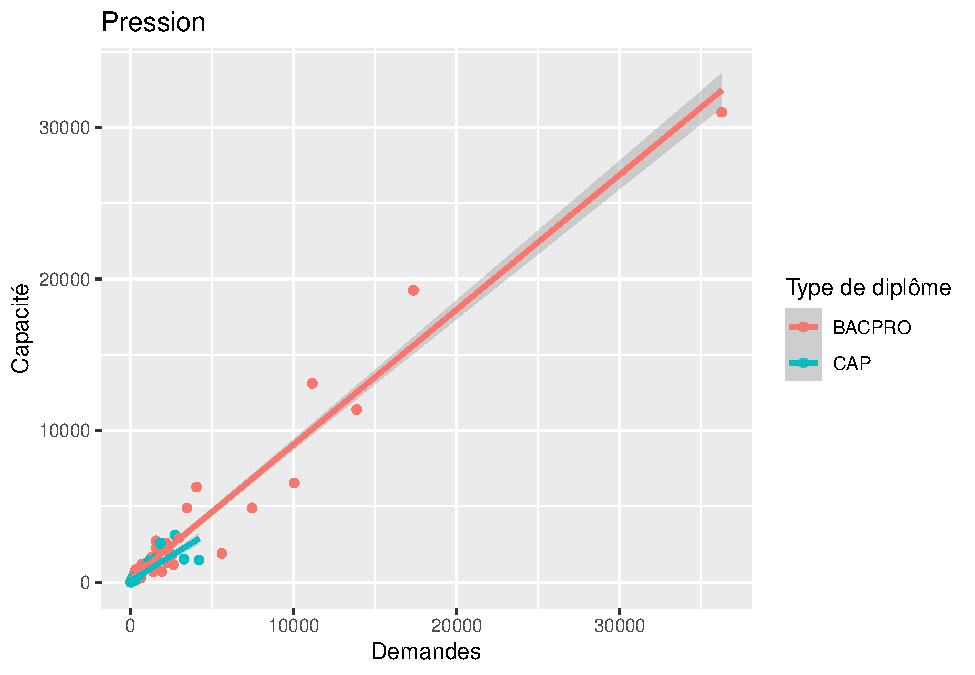
\includegraphics{_main_files/figure-latex/lycee1-1.pdf}

On voit que ça a l'air assez linéaire. Et on voit surtout que certains diplômes
explose les chiffres en terme de demande.

On voit demander à ggplot de passer en log pour mieux faire la différence.

\begin{Shaded}
\begin{Highlighting}[]
\FunctionTok{ggplot}\NormalTok{(lycee,}\FunctionTok{aes}\NormalTok{(Demandes,Capacité,}\AttributeTok{col=}\StringTok{\textasciigrave{}}\AttributeTok{Type de diplôme}\StringTok{\textasciigrave{}}\NormalTok{))}\SpecialCharTok{+}\FunctionTok{geom\_point}\NormalTok{() }\SpecialCharTok{+}
  \FunctionTok{ggtitle}\NormalTok{(}\StringTok{"Pression"}\NormalTok{)}\SpecialCharTok{+}
  \FunctionTok{geom\_smooth}\NormalTok{(}\AttributeTok{method=}\StringTok{"lm"}\NormalTok{) }\SpecialCharTok{+}
  \FunctionTok{scale\_x\_continuous}\NormalTok{(}\AttributeTok{trans =} \StringTok{\textquotesingle{}log2\textquotesingle{}}\NormalTok{) }\SpecialCharTok{+}
  \FunctionTok{scale\_y\_continuous}\NormalTok{(}\AttributeTok{trans =} \StringTok{\textquotesingle{}log2\textquotesingle{}}\NormalTok{)}
\end{Highlighting}
\end{Shaded}

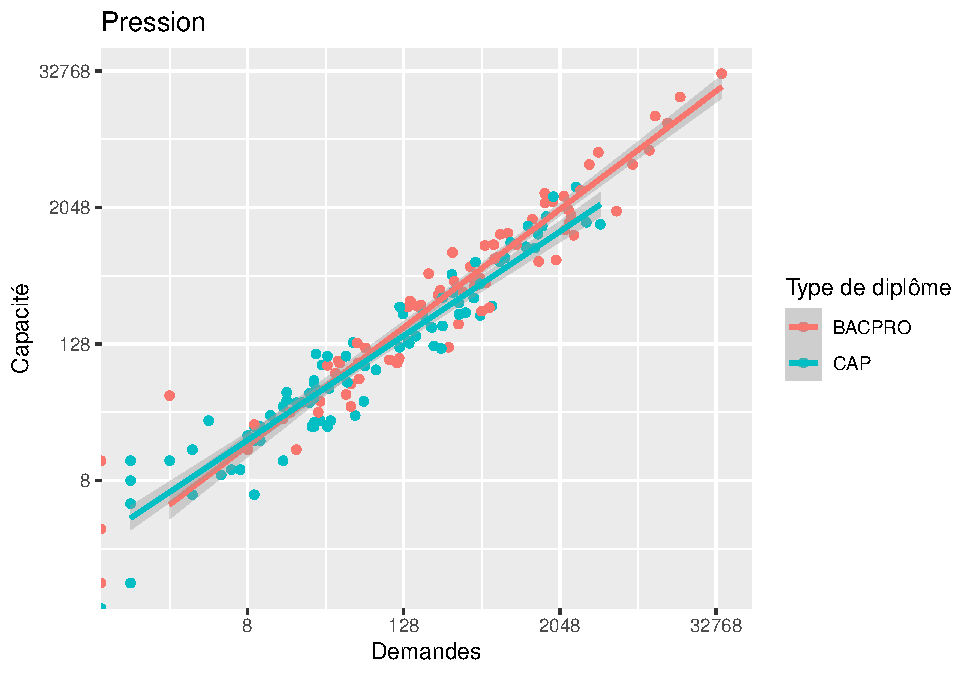
\includegraphics{_main_files/figure-latex/lycee2-1.pdf}

En fait on voit que c'est vers zéro qu'il y a un problème. Ca peut être du au \textbf{log2}.
Mais globalement il n'y a pas d'anomalies à l'oeil.

Et c'est bien logarithmiquement linéaire. Il y a une différence avec plus de capacités
pour les BAC PRO pour les fortes demandes que pour les CAPs où c'est l'inverse.

On regarde le TOP10 des formations en terme de candidats ?

\begin{Shaded}
\begin{Highlighting}[]
\NormalTok{lycee }\SpecialCharTok{\%\textgreater{}\%} \FunctionTok{select}\NormalTok{(}\SpecialCharTok{{-}}\StringTok{\textasciigrave{}}\AttributeTok{Année diplôme}\StringTok{\textasciigrave{}}\NormalTok{,}\SpecialCharTok{{-}}\StringTok{\textasciigrave{}}\AttributeTok{Spécialité libellé}\StringTok{\textasciigrave{}}\NormalTok{,}
                 \SpecialCharTok{{-}}\FunctionTok{starts\_with}\NormalTok{(}\StringTok{"MEFSTAT"}\NormalTok{),}
                 \SpecialCharTok{{-}}\FunctionTok{starts\_with}\NormalTok{(}\StringTok{"Code Diplôme"}\NormalTok{),}
                 \SpecialCharTok{{-}}\StringTok{\textasciigrave{}}\AttributeTok{Année première année}\StringTok{\textasciigrave{}}\NormalTok{) }\SpecialCharTok{\%\textgreater{}\%} \FunctionTok{arrange}\NormalTok{(}\FunctionTok{desc}\NormalTok{(Demandes)) }\SpecialCharTok{\%\textgreater{}\%}
  \FunctionTok{slice}\NormalTok{(}\DecValTok{1}\SpecialCharTok{:}\DecValTok{10}\NormalTok{)}
\end{Highlighting}
\end{Shaded}

\begin{verbatim}
## # A tibble: 10 x 10
##    Diplôme             `Type de diplôme` Filière `Taux d'emploi` `Taux de pression` Demandes Capacité `Code type diplôme`
##    <chr>               <chr>             <chr>             <dbl>              <dbl>    <dbl>    <dbl> <fct>              
##  1 BACPRO VENTE        BACPRO            Relati~            40.9              1.17     36249    31004 400                
##  2 BACPRO ACCUEIL - R~ BACPRO            Relati~            32.8              1.17     36249    31004 400                
##  3 BACPRO COMMERCE     BACPRO            Relati~            41.8              1.17     36249    31004 400                
##  4 BACPRO GESTION-ADM~ BACPRO            Gestio~            31.6              0.901    17346    19255 400                
##  5 BACPRO LOGISTIQUE   BACPRO            Gestio~            42.4              0.901    17346    19255 400                
##  6 BACPRO TRANSPORT    BACPRO            Gestio~            38.7              0.901    17346    19255 400                
##  7 BACPRO ACCOMPAGNEM~ BACPRO            Santé,~            31.1              1.22     13865    11389 400                
##  8 BACPRO METIERS DE ~ BACPRO            Electr~            40.5              0.850    11145    13110 400                
##  9 BACPRO SYSTEMES NU~ BACPRO            Electr~            34.1              1.53     10035     6539 400                
## 10 BACPRO SYSTEMES NU~ BACPRO            Electr~            30.9              1.53     10035     6539 400                
## # i 2 more variables: `Admis apprentissage 2019` <dbl>, `Admis voie scolaire 2019` <dbl>
\end{verbatim}

On regarde maintenant le taux d'emploi au regard du taux de pression :

\begin{Shaded}
\begin{Highlighting}[]
\FunctionTok{ggplot}\NormalTok{(lycee,}\FunctionTok{aes}\NormalTok{(Demandes,}\StringTok{\textasciigrave{}}\AttributeTok{Taux d\textquotesingle{}emploi}\StringTok{\textasciigrave{}}\NormalTok{))}\SpecialCharTok{+}
  \FunctionTok{geom\_point}\NormalTok{() }\SpecialCharTok{+} \FunctionTok{geom\_smooth}\NormalTok{(}\AttributeTok{method=}\StringTok{"lm"}\NormalTok{) }\SpecialCharTok{+} \FunctionTok{facet\_grid}\NormalTok{(}\StringTok{\textasciigrave{}}\AttributeTok{Type de diplôme}\StringTok{\textasciigrave{}} \SpecialCharTok{\textasciitilde{}}\NormalTok{ .) }
\end{Highlighting}
\end{Shaded}

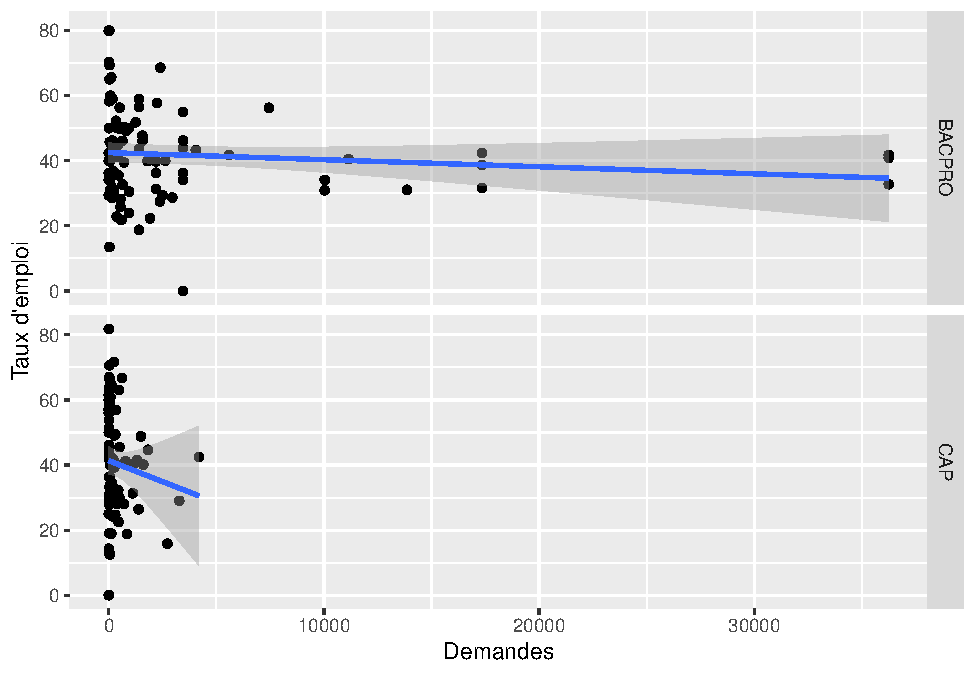
\includegraphics{_main_files/figure-latex/lycee3-1.pdf}
Ouf\ldots{} on s'y attendait pas.

\begin{Shaded}
\begin{Highlighting}[]
\FunctionTok{ggplot}\NormalTok{(lycee,}\FunctionTok{aes}\NormalTok{(Demandes,}\StringTok{\textasciigrave{}}\AttributeTok{Taux d\textquotesingle{}emploi}\StringTok{\textasciigrave{}}\NormalTok{))}\SpecialCharTok{+}
  \FunctionTok{geom\_point}\NormalTok{() }\SpecialCharTok{+} \FunctionTok{geom\_smooth}\NormalTok{() }\SpecialCharTok{+} \FunctionTok{facet\_grid}\NormalTok{(}\StringTok{\textasciigrave{}}\AttributeTok{Type de diplôme}\StringTok{\textasciigrave{}} \SpecialCharTok{\textasciitilde{}}\NormalTok{ .) }\SpecialCharTok{+}
  \FunctionTok{scale\_x\_continuous}\NormalTok{(}\AttributeTok{trans=}\StringTok{"log2"}\NormalTok{)}
\end{Highlighting}
\end{Shaded}

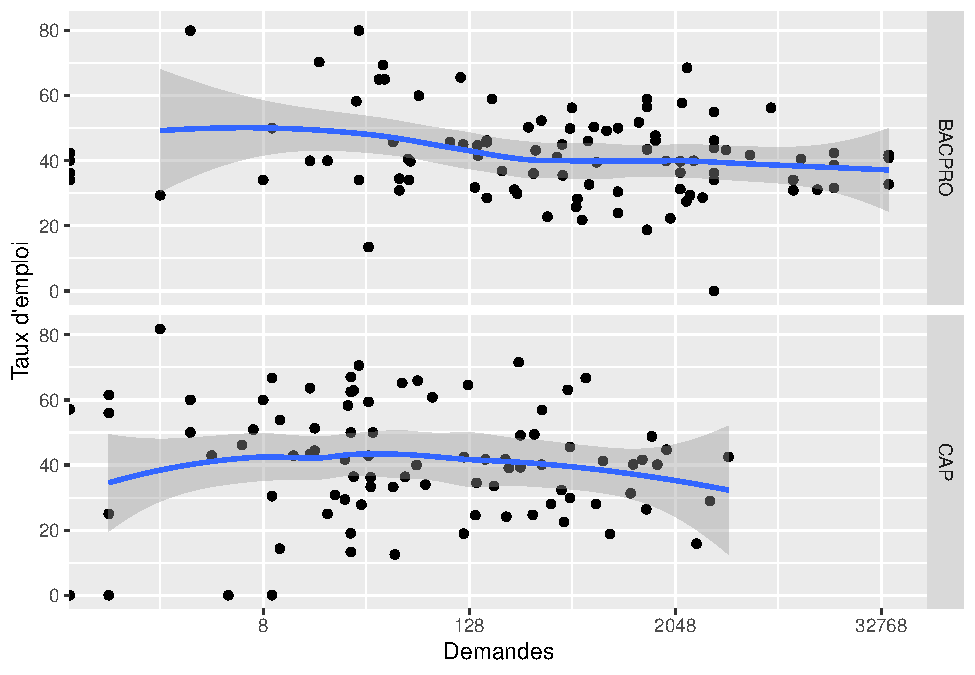
\includegraphics{_main_files/figure-latex/lycee4-1.pdf}
Apparemment il n'y a pas corrélation claire entre le taux de pression et le taux d'emploi.

On a des points extrêmes, on va ajouter les étiquettes.

\begin{Shaded}
\begin{Highlighting}[]
\FunctionTok{ggplot}\NormalTok{(lycee,}\FunctionTok{aes}\NormalTok{(}\StringTok{\textasciigrave{}}\AttributeTok{Taux de pression}\StringTok{\textasciigrave{}}\NormalTok{,}\StringTok{\textasciigrave{}}\AttributeTok{Taux d\textquotesingle{}emploi}\StringTok{\textasciigrave{}}\NormalTok{,}\AttributeTok{label=}\NormalTok{Diplôme))}\SpecialCharTok{+}
  \FunctionTok{geom\_point}\NormalTok{() }\SpecialCharTok{+} \FunctionTok{geom\_smooth}\NormalTok{()  }\SpecialCharTok{+} \FunctionTok{facet\_grid}\NormalTok{(}\StringTok{\textasciigrave{}}\AttributeTok{Type de diplôme}\StringTok{\textasciigrave{}} \SpecialCharTok{\textasciitilde{}}\NormalTok{ .) }\SpecialCharTok{+} 
  \FunctionTok{geom\_text\_repel}\NormalTok{()}
\end{Highlighting}
\end{Shaded}

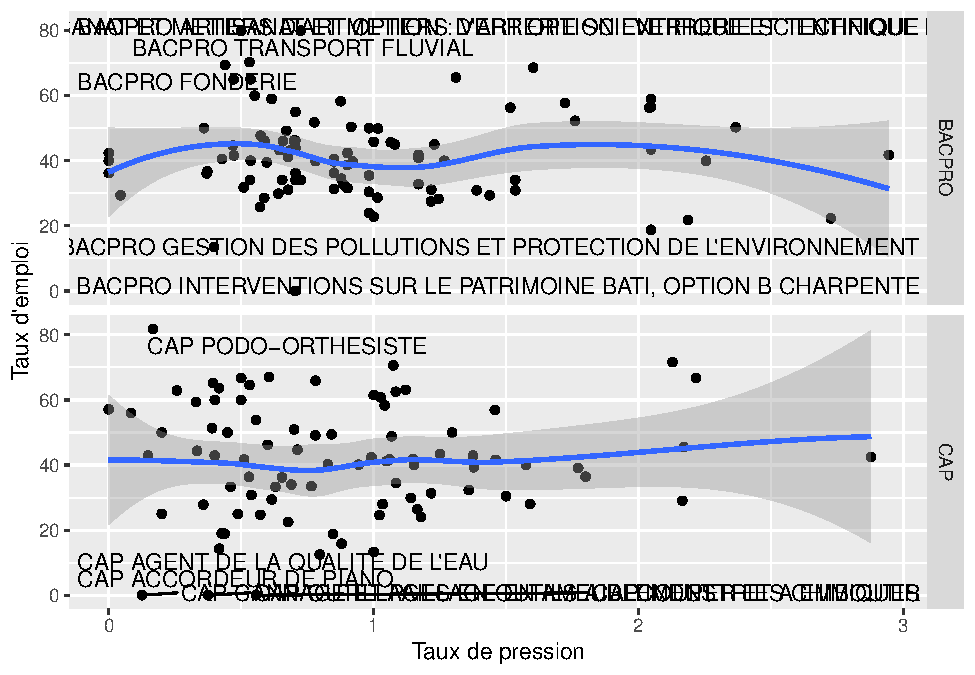
\includegraphics{_main_files/figure-latex/lycee5-1.pdf}
Y'a comme un souci\ldots{}

\begin{Shaded}
\begin{Highlighting}[]
\FunctionTok{ggplot}\NormalTok{(lycee,}\FunctionTok{aes}\NormalTok{(}\StringTok{\textasciigrave{}}\AttributeTok{Taux de pression}\StringTok{\textasciigrave{}}\NormalTok{,}\StringTok{\textasciigrave{}}\AttributeTok{Taux d\textquotesingle{}emploi}\StringTok{\textasciigrave{}}\NormalTok{,}\AttributeTok{label=}\StringTok{\textasciigrave{}}\AttributeTok{Code diplôme...12}\StringTok{\textasciigrave{}}\NormalTok{))}\SpecialCharTok{+}
  \FunctionTok{geom\_point}\NormalTok{() }\SpecialCharTok{+} \FunctionTok{geom\_smooth}\NormalTok{()  }\SpecialCharTok{+} \FunctionTok{facet\_grid}\NormalTok{(}\StringTok{\textasciigrave{}}\AttributeTok{Type de diplôme}\StringTok{\textasciigrave{}} \SpecialCharTok{\textasciitilde{}}\NormalTok{ .) }\SpecialCharTok{+} 
  \FunctionTok{geom\_text\_repel}\NormalTok{()}
\end{Highlighting}
\end{Shaded}

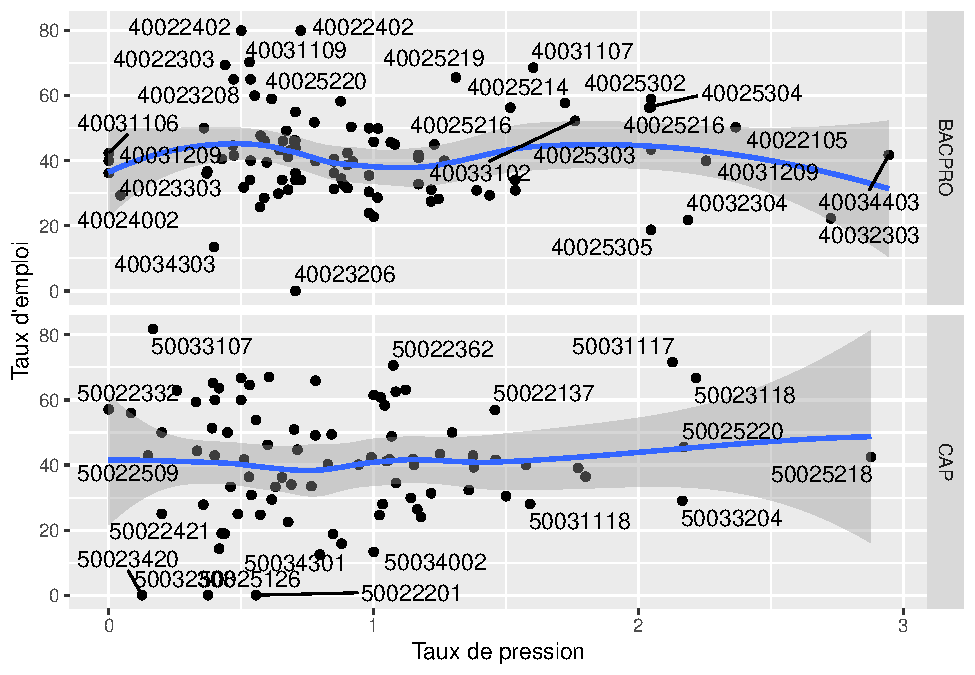
\includegraphics{_main_files/figure-latex/lycee6-1.pdf}

Par exemple :

\begin{Shaded}
\begin{Highlighting}[]
\NormalTok{lycee }\SpecialCharTok{\%\textgreater{}\%} \FunctionTok{select}\NormalTok{(}\SpecialCharTok{{-}}\StringTok{\textasciigrave{}}\AttributeTok{Année diplôme}\StringTok{\textasciigrave{}}\NormalTok{,}\SpecialCharTok{{-}}\StringTok{\textasciigrave{}}\AttributeTok{Spécialité libellé}\StringTok{\textasciigrave{}}\NormalTok{,}
                 \SpecialCharTok{{-}}\FunctionTok{starts\_with}\NormalTok{(}\StringTok{"MEFSTAT"}\NormalTok{),}
                 \SpecialCharTok{{-}}\FunctionTok{starts\_with}\NormalTok{(}\StringTok{"Code Diplôme...15"}\NormalTok{),}
                 \SpecialCharTok{{-}}\StringTok{\textasciigrave{}}\AttributeTok{Année première année}\StringTok{\textasciigrave{}}\NormalTok{) }\SpecialCharTok{\%\textgreater{}\%} 
  \FunctionTok{filter}\NormalTok{(}\StringTok{\textasciigrave{}}\AttributeTok{Code diplôme...12}\StringTok{\textasciigrave{}} \SpecialCharTok{\%in\%} \FunctionTok{c}\NormalTok{(}\DecValTok{40022402}\NormalTok{,}\DecValTok{40023206}\NormalTok{,}\DecValTok{40031109}\NormalTok{,}\DecValTok{50022362}\NormalTok{))}
\end{Highlighting}
\end{Shaded}

\begin{verbatim}
## # A tibble: 5 x 11
##   Diplôme              `Type de diplôme` Filière `Taux d'emploi` `Taux de pression` Demandes Capacité `Code diplôme...12`
##   <chr>                <chr>             <chr>             <dbl>              <dbl>    <dbl>    <dbl> <chr>              
## 1 BACPRO ARTISANAT ET~ BACPRO            Métier~            80                0.5          3        6 40022402           
## 2 CAP ART ET TECHNIQU~ CAP               Métier~            70.6              1.07        29       27 50022362           
## 3 BACPRO ARTISANAT ET~ BACPRO            Métier~            80                0.725       29       40 40022402           
## 4 BACPRO TRANSPORT FL~ BACPRO            Gestio~            70.3              0.531       17       32 40031109           
## 5 BACPRO INTERVENTION~ BACPRO            Constr~             0                0.705     3455     4903 40023206           
## # i 3 more variables: `Code type diplôme` <fct>, `Admis apprentissage 2019` <dbl>, `Admis voie scolaire 2019` <dbl>
\end{verbatim}

Apparemment les charpentiers ne peuvent pas travailler beaucoup.

En fait, on regarde plus systématiquement :

TOP 10 des taux d'emploi :

\begin{Shaded}
\begin{Highlighting}[]
\FunctionTok{kable}\NormalTok{(lycee }\SpecialCharTok{\%\textgreater{}\%} \FunctionTok{group\_by}\NormalTok{(}\StringTok{\textasciigrave{}}\AttributeTok{Type de diplôme}\StringTok{\textasciigrave{}}\NormalTok{) }\SpecialCharTok{\%\textgreater{}\%} \FunctionTok{select}\NormalTok{(}\SpecialCharTok{{-}}\StringTok{\textasciigrave{}}\AttributeTok{Année diplôme}\StringTok{\textasciigrave{}}\NormalTok{,}\SpecialCharTok{{-}}\StringTok{\textasciigrave{}}\AttributeTok{Spécialité libellé}\StringTok{\textasciigrave{}}\NormalTok{,}
                 \SpecialCharTok{{-}}\FunctionTok{starts\_with}\NormalTok{(}\StringTok{"MEFSTAT"}\NormalTok{),}
                 \SpecialCharTok{{-}}\FunctionTok{starts\_with}\NormalTok{(}\StringTok{"Code Diplôme"}\NormalTok{),}
                 \SpecialCharTok{{-}}\StringTok{\textasciigrave{}}\AttributeTok{Année première année}\StringTok{\textasciigrave{}}\NormalTok{) }\SpecialCharTok{\%\textgreater{}\%} \FunctionTok{slice\_max}\NormalTok{(}\StringTok{\textasciigrave{}}\AttributeTok{Taux d\textquotesingle{}emploi}\StringTok{\textasciigrave{}}\NormalTok{,}\AttributeTok{n=}\DecValTok{10}\NormalTok{))}
\end{Highlighting}
\end{Shaded}

\begin{tabular}{l|l|l|r|r|r|r|l|r|r}
\hline
Diplôme & Type de diplôme & Filière & Taux d'emploi & Taux de pression & Demandes & Capacité & Code type diplôme & Admis apprentissage 2019 & Admis voie scolaire 2019\\
\hline
BACPRO ARTISANAT ET METIERS D'ART OPTION : VERRERIE SCIENTIFIQUE ET TECHNIQUE & BACPRO & Métiers d'art & 80.0 & 0.5000000 & 3 & 6 & 400 & 0 & 11\\
\hline
BACPRO ARTISANAT ET METIERS D'ART OPTION : VERRERIE SCIENTIFIQUE ET TECHNIQUE & BACPRO & Métiers d'art & 80.0 & 0.7250000 & 29 & 40 & 400 & 0 & 11\\
\hline
BACPRO TRANSPORT FLUVIAL & BACPRO & Gestion-administration, transport, logistique, sécurité & 70.3 & 0.5312500 & 17 & 32 & 400 & 16 & 23\\
\hline
BACPRO FONDERIE & BACPRO & Productique, mécanique, automatisation & 69.4 & 0.4395604 & 40 & 91 & 400 & 6 & 32\\
\hline
BACPRO CONDUCTEUR TRANSPORT ROUTIER MARCHANDISES & BACPRO & Gestion-administration, transport, logistique, sécurité & 68.6 & 1.6021362 & 2400 & 1498 & 400 & 5 & 1116\\
\hline
BACPRO MAINTENANCE DES MATERIELS OPTION A MATERIELS AGRICOLES & BACPRO & Automobile, engins & 65.6 & 1.3103448 & 114 & 87 & 400 & 281 & 501\\
\hline
BACPRO METIERS ET ARTS DE LA PIERRE & BACPRO & Métiers d'art & 65.0 & 0.4712644 & 41 & 87 & 400 & 7 & 35\\
\hline
BACPRO MAINTENANCE DES MATERIELS OPTION B MATERIELS DE CONSTRUCTION ET DE MANUTENTION & BACPRO & Automobile, engins & 65.0 & 0.5352113 & 38 & 71 & 400 & 137 & 375\\
\hline
BACPRO CONSTRUCTION DES CARROSSERIES & BACPRO & Automobile, engins & 60.0 & 0.5508475 & 65 & 118 & 400 & 23 & 58\\
\hline
BACPRO MAINTENANCE DES VEHICULES OPTION B VEHICULES DE TRANSPORT ROUTIER & BACPRO & Automobile, engins & 59.0 & 0.6148410 & 174 & 283 & 400 & 356 & 440\\
\hline
CAP PODO-ORTHESISTE & CAP & Santé, social, services à la personne et à la collectivité & 81.8 & 0.1666667 & 2 & 12 & 500 & 9 & 5\\
\hline
CAP CONDUCTEUR ROUTIER "MARCHANDISES" & CAP & Gestion-administration, transport, logistique, sécurité & 71.6 & 2.1282051 & 249 & 117 & 500 & 959 & 464\\
\hline
CAP ART ET TECHNIQUES DE LA BIJOUTERIE-JOAILLERIE OPTION BIJOUTERIE-SERTISSAGE & CAP & Métiers d'art & 70.6 & 1.0740741 & 29 & 27 & 500 & 26 & 47\\
\hline
CAP CHOCOLATIER CONFISEUR & CAP & Alimentation, hôtellerie, restauration, tourisme & 67.0 & 0.6046512 & 26 & 43 & 500 & 611 & 86\\
\hline
CAP CONDUCTEUR D'ENGINS : TRAVAUX PUBLICS ET CARRIERES & CAP & Construction, bâtiment, travaux publics & 66.7 & 2.2166065 & 614 & 277 & 500 & 468 & 385\\
\hline
CAP MODELES ET MOULES CERAMIQUES & CAP & Métiers d'art & 66.7 & 0.5000000 & 9 & 18 & 500 & 1 & 5\\
\hline
CAP CONSTRUCTEUR DE ROUTES & CAP & Construction, bâtiment, travaux publics & 65.9 & 0.7804878 & 64 & 82 & 500 & 257 & 25\\
\hline
CAP TAILLEUR DE PIERRE & CAP & Métiers d'art & 65.2 & 0.3939394 & 52 & 132 & 500 & 66 & 52\\
\hline
CAP COUVREUR & CAP & Construction, bâtiment, travaux publics & 64.6 & 0.5316456 & 126 & 237 & 500 & 966 & 108\\
\hline
CAP ARTS ET TECHNIQUES DU VERRE OPTION DECORATEUR & CAP & Métiers d'art & 63.6 & 0.4166667 & 15 & 36 & 500 & 4 & 26\\
\hline
\end{tabular}

et l'inverse

\begin{Shaded}
\begin{Highlighting}[]
\FunctionTok{kable}\NormalTok{(lycee }\SpecialCharTok{\%\textgreater{}\%} \FunctionTok{group\_by}\NormalTok{(}\StringTok{\textasciigrave{}}\AttributeTok{Type de diplôme}\StringTok{\textasciigrave{}}\NormalTok{) }\SpecialCharTok{\%\textgreater{}\%} \FunctionTok{select}\NormalTok{(}\SpecialCharTok{{-}}\StringTok{\textasciigrave{}}\AttributeTok{Année diplôme}\StringTok{\textasciigrave{}}\NormalTok{,}\SpecialCharTok{{-}}\StringTok{\textasciigrave{}}\AttributeTok{Spécialité libellé}\StringTok{\textasciigrave{}}\NormalTok{,}
                 \SpecialCharTok{{-}}\FunctionTok{starts\_with}\NormalTok{(}\StringTok{"MEFSTAT"}\NormalTok{),}
                 \SpecialCharTok{{-}}\FunctionTok{starts\_with}\NormalTok{(}\StringTok{"Code Diplôme"}\NormalTok{),}
                 \SpecialCharTok{{-}}\StringTok{\textasciigrave{}}\AttributeTok{Année première année}\StringTok{\textasciigrave{}}\NormalTok{) }\SpecialCharTok{\%\textgreater{}\%} \FunctionTok{slice\_min}\NormalTok{(}\StringTok{\textasciigrave{}}\AttributeTok{Taux d\textquotesingle{}emploi}\StringTok{\textasciigrave{}}\NormalTok{,}\AttributeTok{n=}\DecValTok{10}\NormalTok{))}
\end{Highlighting}
\end{Shaded}

\begin{tabular}{l|l|l|r|r|r|r|l|r|r}
\hline
Diplôme & Type de diplôme & Filière & Taux d'emploi & Taux de pression & Demandes & Capacité & Code type diplôme & Admis apprentissage 2019 & Admis voie scolaire 2019\\
\hline
BACPRO INTERVENTIONS SUR LE PATRIMOINE BATI, OPTION B CHARPENTE & BACPRO & Construction, bâtiment, travaux publics & 0.0 & 0.7046706 & 3455 & 4903 & 400 & 1 & 8\\
\hline
BACPRO GESTION DES POLLUTIONS ET PROTECTION DE L'ENVIRONNEMENT & BACPRO & Electricité, électronique/numérique, environnement & 13.5 & 0.3975904 & 33 & 83 & 400 & 6 & 55\\
\hline
BACPRO AVIATION GENERALE & BACPRO & Aéronautique & 18.8 & 2.0467153 & 1402 & 685 & 400 & 4 & 20\\
\hline
BACPRO PHOTOGRAPHIE & BACPRO & Industries graphiques, communication, audiovisuel, spectacle & 21.8 & 2.1865672 & 586 & 268 & 400 & 7 & 300\\
\hline
BACPRO ARTISANAT ET METIERS D'ART OPTION : COMMUNICATION VISUELLE PLURI-MEDIA & BACPRO & Industries graphiques, communication, audiovisuel, spectacle & 22.3 & 2.7258523 & 1919 & 704 & 400 & 33 & 1322\\
\hline
BACPRO ARTISANAT ET METIERS D'ART OPTION MARCHANDISAGE VISUEL & BACPRO & Industries graphiques, communication, audiovisuel, spectacle & 22.8 & 1.0000000 & 367 & 367 & 400 & 0 & 308\\
\hline
BACPRO REALISATION DE PRODUITS IMPRIMES ET PLURIMEDIA OPTION A PRODUCTIONS GRAPHIQUES & BACPRO & Industries graphiques, communication, audiovisuel, spectacle & 23.9 & 0.9823651 & 947 & 964 & 400 & 54 & 514\\
\hline
BACPRO ETUDE ET DEFINITION DE PRODUITS INDUSTRIELS & BACPRO & Productique, mécanique, automatisation & 25.8 & 0.5706751 & 541 & 948 & 400 & 0 & 523\\
\hline
BACPRO SERVICES DE PROXIMITE ET VIE LOCALE & BACPRO & Santé, social, services à la personne et à la collectivité & 27.5 & 1.2163683 & 2378 & 1955 & 400 & 5 & 2187\\
\hline
BACPRO ETUDE ET REALISATION D'AGENCEMENT & BACPRO & Construction, bâtiment, travaux publics & 28.3 & 1.2448980 & 549 & 441 & 400 & 0 & 303\\
\hline
CAP OUTILLAGES EN OUTILS A DECOUPER ET A EMBOUTIR & CAP & Productique, mécanique, automatisation & 0.0 & 0.3750000 & 9 & 24 & 500 & 0 & 11\\
\hline
CAP ASSISTANT TECHNIQUE EN INSTRUMENTS DE MUSIQUE OPTION GUITARE & CAP & Industries graphiques, communication, audiovisuel, spectacle & 0.0 & NA & 0 & 0 & 500 & 6 & 12\\
\hline
CAP CANNAGE ET PAILLAGE EN AMEUBLEMENT & CAP & Métiers d'art & 0.0 & 0.1250000 & 1 & 8 & 500 & 0 & 1\\
\hline
CAP ACCORDEUR DE PIANO & CAP & Industries graphiques, communication, audiovisuel, spectacle & 0.0 & 0.1250000 & 1 & 8 & 500 & 0 & 5\\
\hline
CAP INDUSTRIES CHIMIQUES & CAP & Biochimie industrielle & 0.0 & 0.5555556 & 5 & 9 & 500 & 0 & 7\\
\hline
CAP AGENT DE LA QUALITE DE L'EAU & CAP & Electricité, électronique/numérique, environnement & 12.5 & 0.7966102 & 47 & 59 & 500 & 0 & 35\\
\hline
CAP AGENT DE PREVENTION ET DE MEDIATION & CAP & Santé, social, services à la personne et à la collectivité & 13.3 & 1.0000000 & 26 & 26 & 500 & 0 & 2305\\
\hline
CAP TOURNAGE EN CERAMIQUE & CAP & Métiers d'art & 14.3 & 0.4166667 & 10 & 24 & 500 & 3 & 19\\
\hline
CAP ASSISTANT(E) TECHNIQUE EN MILIEUX FAMILIAL ET COLLECTIF & CAP & Santé, social, services à la personne et à la collectivité & 15.8 & 0.8788660 & 2728 & 3104 & 500 & 43 & 2810\\
\hline
CAP METIERS DE LA MODE-VÊTEMENT FLOU & CAP & Textile, habillement, cuir & 18.8 & 0.8470705 & 853 & 1007 & 500 & 26 & 699\\
\hline
\end{tabular}

Est-ce qu'il y a un lien entre l'effectif et le taux d'emploi ?

\begin{Shaded}
\begin{Highlighting}[]
\FunctionTok{ggplot}\NormalTok{(lycee,}\FunctionTok{aes}\NormalTok{(}\StringTok{\textasciigrave{}}\AttributeTok{Taux de pression}\StringTok{\textasciigrave{}}\NormalTok{,}\StringTok{\textasciigrave{}}\AttributeTok{Demandes}\StringTok{\textasciigrave{}}\NormalTok{))}\SpecialCharTok{+}
  \FunctionTok{geom\_point}\NormalTok{() }\SpecialCharTok{+} \FunctionTok{geom\_smooth}\NormalTok{()  }\SpecialCharTok{+} \FunctionTok{facet\_grid}\NormalTok{(}\StringTok{\textasciigrave{}}\AttributeTok{Type de diplôme}\StringTok{\textasciigrave{}} \SpecialCharTok{\textasciitilde{}}\NormalTok{ .) }
\end{Highlighting}
\end{Shaded}

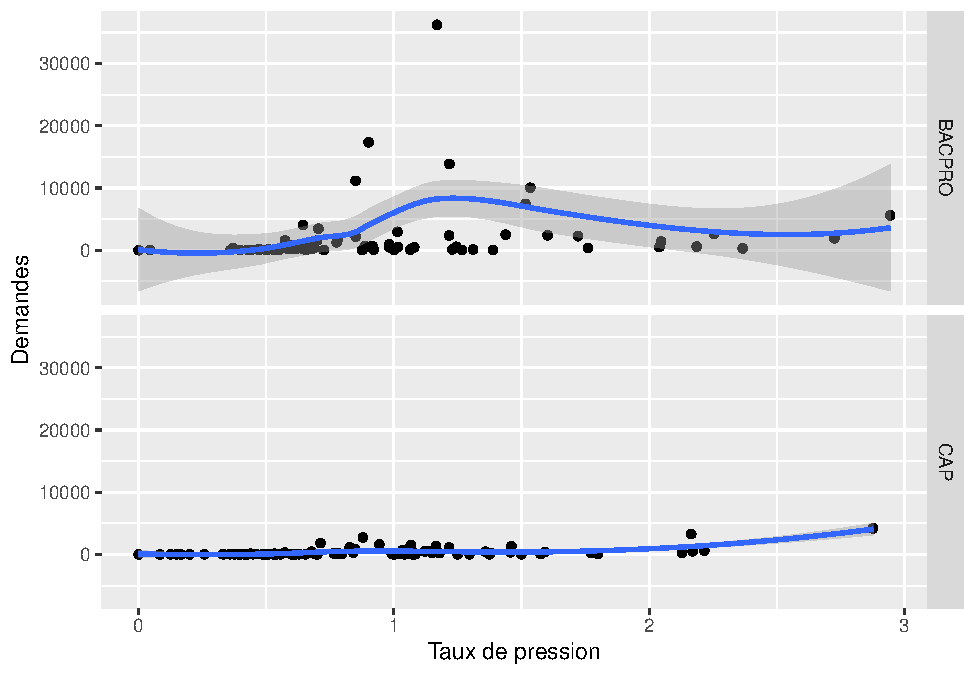
\includegraphics{_main_files/figure-latex/lycee7-1.pdf}
Il faut qu'on retourne aux \textbf{log2}.

\begin{Shaded}
\begin{Highlighting}[]
\FunctionTok{ggplot}\NormalTok{(lycee,}\FunctionTok{aes}\NormalTok{(}\StringTok{\textasciigrave{}}\AttributeTok{Taux de pression}\StringTok{\textasciigrave{}}\NormalTok{,}\StringTok{\textasciigrave{}}\AttributeTok{Demandes}\StringTok{\textasciigrave{}}\NormalTok{))}\SpecialCharTok{+}
  \FunctionTok{geom\_point}\NormalTok{() }\SpecialCharTok{+} \FunctionTok{geom\_smooth}\NormalTok{()  }\SpecialCharTok{+} \FunctionTok{facet\_grid}\NormalTok{(}\StringTok{\textasciigrave{}}\AttributeTok{Type de diplôme}\StringTok{\textasciigrave{}} \SpecialCharTok{\textasciitilde{}}\NormalTok{ .) }\SpecialCharTok{+}
  \FunctionTok{scale\_y\_continuous}\NormalTok{(}\AttributeTok{trans=}\StringTok{"log2"}\NormalTok{)}
\end{Highlighting}
\end{Shaded}

\includegraphics{_main_files/figure-latex/lycee8-1.pdf}
Apparemment oui mais ce n'est pas linéaire.

Pour faire un graphique avec le taux moyen d'emploi selon la filière ?

\begin{Shaded}
\begin{Highlighting}[]
\NormalTok{graphique }\OtherTok{\textless{}{-}}\NormalTok{ lycee }\SpecialCharTok{\%\textgreater{}\%} \FunctionTok{group\_by}\NormalTok{(Filière) }\SpecialCharTok{\%\textgreater{}\%} 
  \FunctionTok{summarise}\NormalTok{(}\AttributeTok{Moyenne=}\FunctionTok{mean}\NormalTok{(}\StringTok{\textasciigrave{}}\AttributeTok{Taux d\textquotesingle{}emploi}\StringTok{\textasciigrave{}}\NormalTok{))}

\FunctionTok{ggplot}\NormalTok{(graphique,}\FunctionTok{aes}\NormalTok{(Filière,Moyenne,}\AttributeTok{fill=}\NormalTok{Filière)) }\SpecialCharTok{+} \FunctionTok{geom\_bar}\NormalTok{(}\AttributeTok{color=}\StringTok{"black"}\NormalTok{,}\AttributeTok{stat=}\StringTok{"identity"}\NormalTok{)}
\end{Highlighting}
\end{Shaded}

\includegraphics{_main_files/figure-latex/lycee10-1.pdf}
on enlève l'axe des abscisses\ldots{}

\begin{Shaded}
\begin{Highlighting}[]
\NormalTok{graphique }\OtherTok{\textless{}{-}}\NormalTok{ lycee }\SpecialCharTok{\%\textgreater{}\%} \FunctionTok{group\_by}\NormalTok{(Filière) }\SpecialCharTok{\%\textgreater{}\%} 
  \FunctionTok{summarise}\NormalTok{(}\AttributeTok{Moyenne=}\FunctionTok{mean}\NormalTok{(}\StringTok{\textasciigrave{}}\AttributeTok{Taux d\textquotesingle{}emploi}\StringTok{\textasciigrave{}}\NormalTok{))}

\FunctionTok{ggplot}\NormalTok{(graphique,}\FunctionTok{aes}\NormalTok{(Filière,Moyenne,}\AttributeTok{fill=}\NormalTok{Filière)) }\SpecialCharTok{+} \FunctionTok{geom\_bar}\NormalTok{(}\AttributeTok{color=}\StringTok{"black"}\NormalTok{,}\AttributeTok{stat=}\StringTok{"identity"}\NormalTok{) }\SpecialCharTok{+}
   \FunctionTok{theme}\NormalTok{(}\AttributeTok{axis.title.x=}\FunctionTok{element\_blank}\NormalTok{(),}
        \AttributeTok{axis.text.x=}\FunctionTok{element\_blank}\NormalTok{(),}
        \AttributeTok{axis.ticks.x=}\FunctionTok{element\_blank}\NormalTok{())}
\end{Highlighting}
\end{Shaded}

\includegraphics{_main_files/figure-latex/lycee11-1.pdf}

\hypertarget{commentaires-des-auditeurs}{%
\section{Commentaires des auditeurs}\label{commentaires-des-auditeurs}}

Deux problèmes ont été signalés par les doctorants dans l'analyse qui interrogent
sur la documentation voire la qualité des données :

\begin{itemize}
\tightlist
\item
  il y a le fait, que la première table abrite plusieurs occurences pour le même
  libellé de diplôme, MEFTSTAT, \ldots{} Ce qui est curieux
\end{itemize}

\begin{Shaded}
\begin{Highlighting}[]
\NormalTok{a}\OtherTok{=}\FunctionTok{table}\NormalTok{(lycee}\SpecialCharTok{$}\StringTok{\textasciigrave{}}\AttributeTok{Spécialité libellé}\StringTok{\textasciigrave{}}\NormalTok{)}
\NormalTok{a[a}\SpecialCharTok{\textgreater{}}\DecValTok{1}\NormalTok{]}
\end{Highlighting}
\end{Shaded}

\begin{verbatim}
## 
##                              ACCOMPAGNEMENT SOINS ET SERVICES A LA PERSONNE OPTION A - A DOMICILE 
##                                                                                                 2 
##                                                                     AERONAUTIQUE OPTION AVIONIQUE 
##                                                                                                 2 
##                                                              AMENAGEMENT ET FINITIONS DU BATIMENT 
##                                                                                                 2 
##                   ARTISANAT ET METIERS D'ART OPTION : METIERS DE L'ENSEIGNE ET DE LA SIGNALETIQUE 
##                                                                                                 2 
##                            ARTISANAT ET METIERS D'ART OPTION : VERRERIE SCIENTIFIQUE ET TECHNIQUE 
##                                                                                                 2 
##                                                                                        LOGISTIQUE 
##                                                                                                 2 
##                                            MAINTENANCE DES MATERIELS OPTION A MATERIELS AGRICOLES 
##                                                                                                 2 
##                    MAINTENANCE DES MATERIELS OPTION B MATERIELS DE CONSTRUCTION ET DE MANUTENTION 
##                                                                                                 2 
##                                      MAINTENANCE DES MATERIELS OPTION C MATERIELS D'ESPACES VERTS 
##                                                                                                 2 
##                                         MAINTENANCE DES VEHICULES OPTION A VOITURES PARTICULIERES 
##                                                                                                 2 
##                                 MAINTENANCE DES VEHICULES OPTION B VEHICULES DE TRANSPORT ROUTIER 
##                                                                                                 2 
##                                                     MAINTENANCE DES VEHICULES OPTION C MOTOCYCLES 
##                                                                                                 2 
##                                                                        MENUISERIE ALUMINIUM-VERRE 
##                                                                                                 2 
##                                                               METIERS DU CUIR OPTION MAROQUINERIE 
##                                                                                                 2 
##                                                                     POISSONNIER-ECAILLER-TRAITEUR 
##                                                                                                 2 
##                                                                       REPARATION DES CARROSSERIES 
##                                                                                                 2 
## SYSTEMES NUMERIQUES OPTION A SURETE ET SECURITE DES INFRASTRUCTURES, DE L'HABITAT ET DU TERTIAIRE 
##                                                                                                 2 
##                       SYSTEMES NUMERIQUES OPTION C RESEAUX INFORMATIQUES ET SYSTEMES COMMUNICANTS 
##                                                                                                 2 
##                                     TECHNICIEN D'ETUDES DU BATIMENT OPTION A : ETUDES ET ECONOMIE 
##                                                                                                 2
\end{verbatim}

\begin{itemize}
\tightlist
\item
  Il y a des taux d'emploi offerts nuls pour certaines catégories qui sont curieux.
  Par exemple il y le cas pour la construction et le batiment avec pourtant un
  nombre de formés parmi les plus élevés.
\end{itemize}

\hypertarget{quiz..}{%
\section{Quiz..}\label{quiz..}}

\begin{itemize}
\item
  Faire les TOP10 et l'inverse pour les Taux de pression
\item
  Faire le graphique du taux moyen selon la Filières du Taux de pression
\end{itemize}

\hypertarget{donnuxe9es-des-ruxe9serves-parlementaires}{%
\chapter{Données des réserves parlementaires}\label{donnuxe9es-des-ruxe9serves-parlementaires}}

Dans cette partie, on étudie l'utilisation de la réserve parlementaire par les
députés.

Ce sont les \href{https://www.data.gouv.fr/fr/datasets/reserve-parlementaire/}{données de 2014}

Les questions sont celles d'une personne naïve et sans a priori :

\begin{itemize}
\item
  Est-ce que les groupes ont dépensé chacun autant ?
\item
  Est-ce que les groupes ont dépensé chacun autant en moyenne ?
\item
  Est-ce vrai pour les députés en moyenne ? IdAuteur
\item
  Quel est l'enveloppe dépensé au total ?
\end{itemize}

\begin{itemize}
\tightlist
\item
  Est-ce possible avec le descriptif d'avoir les mots-clefs pour les sous dépensés ?
\end{itemize}

\begin{Shaded}
\begin{Highlighting}[]
\NormalTok{reserve }\OtherTok{\textless{}{-}} \FunctionTok{fromJSON}\NormalTok{(}\StringTok{"data/reserve/2014\_reserve\_parlementaire.json"}\NormalTok{)}

\FunctionTok{str}\NormalTok{(reserve)}
\end{Highlighting}
\end{Shaded}

\begin{verbatim}
## 'data.frame':    13133 obs. of  10 variables:
##  $ Bénéficiaire        : chr  "Télé Bocal" "Mieux se déplacer à Bicyclette" "Festival du livre et de la presse d'écologie" "ARDHIS" ...
##  $ Adresse             : chr  "Maison des associations\n1/3 rue Frédérique Lemaître\n75020 Paris" "MDB –\n37 boulevard Bourdon\n75004 Paris" "6 cité de l’Ermitage\n75020 Paris" "76 cours de Vincennes\n75012 Paris" ...
##  $ Descriptif          : chr  "Mise en œuvre d'ateliers de production locale proposant d’utiliser l'image comme une valorisation du travail des artistes" "Réalisation des supports de communication pour faire connaître ses nouvelles dispositions sur l'usage de la bic"| __truncated__ "Organisation du Festival du livre et de la presse d’écologie Promotion du livre et de l’écrit, information, sen"| __truncated__ "Mise en place d’outils de communication : plaquette multilingue qui pourrait être mise à disposition dans les d"| __truncated__ ...
##  $ Montant             : int  5000 4000 3500 2500 5000 2000 3000 2000 10000 8000 ...
##  $ Nom                 : chr  "BAUPIN" "BAUPIN" "BAUPIN" "BAUPIN" ...
##  $ Prénom              : chr  "Denis" "Denis" "Denis" "Denis" ...
##  $ Département         : chr  "Paris" "Paris" "Paris" "Paris" ...
##  $ Groupe              : chr  "Ecolo" "Ecolo" "Ecolo" "Ecolo" ...
##  $ Programme budgétaire: chr  "313-03" "203-15" "334-01" "177-11" ...
##  $ ID_Acteur           : chr  "PA609016" "PA609016" "PA609016" "PA609016" ...
\end{verbatim}

Pourquoi c'est compliqué de faire un gtsummary direct ?

En fait on va se demander si il y a un bénéficiaire qui apparait plusieurs fois.

\hypertarget{buxe9nuxe9ficiaires}{%
\section{Bénéficiaires}\label{buxe9nuxe9ficiaires}}

\begin{Shaded}
\begin{Highlighting}[]
\NormalTok{tb }\OtherTok{\textless{}{-}} \FunctionTok{table}\NormalTok{(reserve}\SpecialCharTok{$}\NormalTok{Bénéficiaire)}
\NormalTok{tb1 }\OtherTok{\textless{}{-}}\NormalTok{ tb[tb}\SpecialCharTok{\textgreater{}}\DecValTok{1}\NormalTok{]}
\FunctionTok{length}\NormalTok{(tb1)}
\end{Highlighting}
\end{Shaded}

\begin{verbatim}
## [1] 267
\end{verbatim}

Si oui, est-ce qu'on peut le mettre sous forme de data.frame ? Pourquoi on a
besoin d'une data.frame pour représenter graphiquement ces informations ?

\begin{Shaded}
\begin{Highlighting}[]
\NormalTok{dt }\OtherTok{\textless{}{-}} \FunctionTok{data.frame}\NormalTok{(}\AttributeTok{Nom=}\FunctionTok{names}\NormalTok{(tb),}\AttributeTok{Nombre=}\FunctionTok{as.numeric}\NormalTok{(tb))}
\FunctionTok{str}\NormalTok{(dt)}
\end{Highlighting}
\end{Shaded}

\begin{verbatim}
## 'data.frame':    12718 obs. of  2 variables:
##  $ Nom   : chr  "\"Le Tracteur\" - Compagnie Beaudrain de paroi" "\"Petite enfance\net soutien\nà la parentalité\"" "(A.R.A.C.) Section Saint-Marcel" "« La Bande à Michel » section théâtre du Foyer Laïque" ...
##  $ Nombre: num  1 1 1 1 1 1 1 1 1 1 ...
\end{verbatim}

Une représentation visuelle de la répartition du nombre sur ceux qui ont plus de
2 donations et après sur l'ensemble.

\begin{Shaded}
\begin{Highlighting}[]
\FunctionTok{ggplot}\NormalTok{(dt,}\FunctionTok{aes}\NormalTok{(Nombre))}\SpecialCharTok{+}\FunctionTok{geom\_histogram}\NormalTok{()}
\end{Highlighting}
\end{Shaded}

\includegraphics{_main_files/figure-latex/reserve1-1.pdf}

Quels sont les bénéficiaires de plus de 5 donations ? Ce sont des termes génériques
ou des entités ?

\begin{Shaded}
\begin{Highlighting}[]
\NormalTok{tbt }\OtherTok{\textless{}{-}} \FunctionTok{table}\NormalTok{(reserve}\SpecialCharTok{$}\NormalTok{Bénéficiaire)}
\NormalTok{dt }\OtherTok{\textless{}{-}} \FunctionTok{data.frame}\NormalTok{(}\AttributeTok{Nom=}\FunctionTok{names}\NormalTok{(tbt),}\AttributeTok{Nombre=}\FunctionTok{as.numeric}\NormalTok{(tbt))}
\NormalTok{dt[dt}\SpecialCharTok{$}\NormalTok{Nombre}\SpecialCharTok{\textgreater{}}\DecValTok{5}\NormalTok{,]}
\end{Highlighting}
\end{Shaded}

\begin{verbatim}
##                          Nom Nombre
## 325                    AIDES      6
## 2927               BRIGNOLES      6
## 3982        Comité des Fêtes      7
## 4475        Commune de Crest      8
## 6416                   FNACA      7
## 8060               Le Refuge     11
## 10509         Restos du Cœur      6
## 11095     Secours catholique      9
## 11096     Secours Catholique      6
## 11116      Secours Populaire     12
## 11527 Sou des Ecoles Laïques      7
\end{verbatim}

\begin{Shaded}
\begin{Highlighting}[]
\NormalTok{tbt }\OtherTok{\textless{}{-}} \FunctionTok{table}\NormalTok{(reserve}\SpecialCharTok{$}\NormalTok{Bénéficiaire)}
\NormalTok{dt }\OtherTok{\textless{}{-}} \FunctionTok{data.frame}\NormalTok{(}\AttributeTok{Nom=}\FunctionTok{names}\NormalTok{(tbt),}\AttributeTok{Nombre=}\FunctionTok{as.numeric}\NormalTok{(tbt))}
\FunctionTok{ggplot}\NormalTok{(dt,}\FunctionTok{aes}\NormalTok{(Nombre))}\SpecialCharTok{+}\FunctionTok{geom\_histogram}\NormalTok{()}
\end{Highlighting}
\end{Shaded}

\includegraphics{_main_files/figure-latex/reserve2-1.pdf}

\hypertarget{par-groupe-politique}{%
\section{Par groupe politique}\label{par-groupe-politique}}

Si on regarde les dépenses par groupe.

\begin{Shaded}
\begin{Highlighting}[]
\FunctionTok{ggplot}\NormalTok{(dt,}\FunctionTok{aes}\NormalTok{(Nombre))}\SpecialCharTok{+}\FunctionTok{geom\_histogram}\NormalTok{()}\SpecialCharTok{+}\FunctionTok{scale\_y\_log10}\NormalTok{()}
\end{Highlighting}
\end{Shaded}

\includegraphics{_main_files/figure-latex/reserve3-1.pdf}

\begin{Shaded}
\begin{Highlighting}[]
\FunctionTok{ggplot}\NormalTok{(reserve,}\FunctionTok{aes}\NormalTok{(Groupe,Montant))}\SpecialCharTok{+}\FunctionTok{geom\_bar}\NormalTok{(}\AttributeTok{stat=}\StringTok{"identity"}\NormalTok{,}\AttributeTok{position=}\StringTok{"dodge"}\NormalTok{)}
\end{Highlighting}
\end{Shaded}

\includegraphics{_main_files/figure-latex/reserve4-1.pdf}

Mais que ?

\begin{Shaded}
\begin{Highlighting}[]
\FunctionTok{table}\NormalTok{(reserve}\SpecialCharTok{$}\NormalTok{Groupe)}
\end{Highlighting}
\end{Shaded}

\begin{verbatim}
## 
##       Ecolo   GDR    NI  RRDP   SRC   UDI   UMP 
##    52   549   148   128   262  5172   741  6081
\end{verbatim}

Il faut trouver et corriger.

\begin{Shaded}
\begin{Highlighting}[]
\NormalTok{maisque }\OtherTok{\textless{}{-}}\NormalTok{ reserve }\SpecialCharTok{\%\textgreater{}\%} \FunctionTok{filter}\NormalTok{(Groupe}\SpecialCharTok{==}\StringTok{""}\NormalTok{)}

\FunctionTok{table}\NormalTok{(maisque}\SpecialCharTok{$}\NormalTok{Nom)}
\end{Highlighting}
\end{Shaded}

\begin{verbatim}
## 
## Présidence de l'Assemblée nationale 
##                                  52
\end{verbatim}

\begin{Shaded}
\begin{Highlighting}[]
\FunctionTok{table}\NormalTok{(maisque}\SpecialCharTok{$}\NormalTok{Descriptif)}
\end{Highlighting}
\end{Shaded}

\begin{verbatim}
## 
## Agir en faveur de l'emploi des jeunes diplômés issus des quartiers prioritaires ou de milieux sociaux défavorisés. 
##                                                                                                                  1 
##                                                            Association de juriste dans la lutte contre l'exclusion 
##                                                                                                                  1 
##                                                  Création d'un système d'information pour le réseau Habitat Jeunes 
##                                                                                                                  1 
##                                                Equipement du futur 3ème siège de l'Alliance française de la Havane 
##                                                                                                                  1 
##                                                                                                     Fonctionnement 
##                                                                                                                 44 
##                                                                                  Fonctionnement Mardis de l'Avenir 
##                                                                                                                  1 
##                                                                  Insertion sociale et professionnelle par le sport 
##                                                                                                                  1 
##                                                                Soutien projet consacré aux femmes de l'immigration 
##                                                                                                                  1 
##                                                                                            Travaux d'intérêt local 
##                                                                                                                  1
\end{verbatim}

\begin{Shaded}
\begin{Highlighting}[]
\NormalTok{reserve }\OtherTok{\textless{}{-}}\NormalTok{ reserve }\SpecialCharTok{\%\textgreater{}\%} \FunctionTok{mutate}\NormalTok{(}\AttributeTok{Groupe=}\FunctionTok{ifelse}\NormalTok{(Groupe}\SpecialCharTok{==}\StringTok{""}\NormalTok{,}\StringTok{"Présidence AN"}\NormalTok{,Groupe))}
\end{Highlighting}
\end{Shaded}

L'erreur corrigée

\begin{Shaded}
\begin{Highlighting}[]
\FunctionTok{ggplot}\NormalTok{(reserve,}\FunctionTok{aes}\NormalTok{(Groupe,Montant))}\SpecialCharTok{+}\FunctionTok{geom\_bar}\NormalTok{(}\AttributeTok{stat=}\StringTok{"identity"}\NormalTok{,}\AttributeTok{position=}\StringTok{"dodge"}\NormalTok{)}
\end{Highlighting}
\end{Shaded}

\includegraphics{_main_files/figure-latex/reserve5-1.pdf}

Les résultats par groupe avec gtsummary ou summarize.

on en profite pour calculer la somme des donations, la donation moyenne par
Acteur et le nombre d'acteur par groupe

\begin{Shaded}
\begin{Highlighting}[]
\NormalTok{groupe }\OtherTok{\textless{}{-}}\NormalTok{ reserve }\SpecialCharTok{\%\textgreater{}\%} \FunctionTok{group\_by}\NormalTok{(Groupe)}

\NormalTok{res }\OtherTok{\textless{}{-}}\NormalTok{ groupe }\SpecialCharTok{\%\textgreater{}\%} \FunctionTok{summarize}\NormalTok{(}\AttributeTok{min=}\FunctionTok{min}\NormalTok{(Montant),}\AttributeTok{max=}\FunctionTok{max}\NormalTok{(Montant),}
                     \AttributeTok{Moyenne=}\FunctionTok{mean}\NormalTok{(Montant),}\AttributeTok{EC=}\FunctionTok{sd}\NormalTok{(Montant),}
                     \AttributeTok{Somme=}\FunctionTok{sum}\NormalTok{(Montant),}\AttributeTok{nbActeur=}\FunctionTok{length}\NormalTok{(}\FunctionTok{unique}\NormalTok{(ID\_Acteur)),}
                     \AttributeTok{Somme\_par\_acteur=}\NormalTok{Somme}\SpecialCharTok{/}\NormalTok{nbActeur)}
\NormalTok{res }
\end{Highlighting}
\end{Shaded}

\begin{verbatim}
## # A tibble: 8 x 8
##   Groupe          min    max Moyenne     EC    Somme nbActeur Somme_par_acteur
##   <chr>         <int>  <int>   <dbl>  <dbl>    <int>    <int>            <dbl>
## 1 Ecolo           500  50000   4805.  4039.  2637890       18          146549.
## 2 GDR              67 130000  14198. 18951.  2101366       16          131335.
## 3 NI              800  90000   8926. 10212.  1142574        9          126953.
## 4 Présidence AN  1000 250000  54923. 53608.  2856000        1         2856000 
## 5 RRDP            650  98000   8813. 11365.  2309018       18          128279.
## 6 SRC             300 190000   7797. 10387. 40323770      290          139047.
## 7 UDI             960  88000   5523.  6880.  4092383       31          132012.
## 8 UMP             240 200000   4047.  7410. 24608557      200          123043.
\end{verbatim}

\hypertarget{exportation-1}{%
\section{Exportation}\label{exportation-1}}

Comment l'exporter pour ses collègues ?

\begin{Shaded}
\begin{Highlighting}[]
\FunctionTok{require}\NormalTok{(writexl)}
\FunctionTok{write\_xlsx}\NormalTok{(res,}\StringTok{"Résultats/Résultats{-}Deputes{-}Reserve.xlsx"}\NormalTok{)}
\end{Highlighting}
\end{Shaded}

\hypertarget{les-sommes-par-acteurs}{%
\section{Les sommes par acteurs}\label{les-sommes-par-acteurs}}

Les sommes par acteurs selon les groupes

\begin{Shaded}
\begin{Highlighting}[]
\FunctionTok{ggplot}\NormalTok{(res }\SpecialCharTok{\%\textgreater{}\%} \FunctionTok{filter}\NormalTok{(nbActeur }\SpecialCharTok{!=} \DecValTok{1}\NormalTok{),}\FunctionTok{aes}\NormalTok{(}\AttributeTok{x=}\NormalTok{Groupe,}\AttributeTok{y=}\NormalTok{Somme\_par\_acteur,}\AttributeTok{fill=}\NormalTok{Groupe))}\SpecialCharTok{+}
  \FunctionTok{geom\_bar}\NormalTok{(,}\AttributeTok{stat=}\StringTok{"identity"}\NormalTok{,}\AttributeTok{position=}\StringTok{"dodge"}\NormalTok{)}
\end{Highlighting}
\end{Shaded}

\includegraphics{_main_files/figure-latex/reserve6-1.pdf}

\hypertarget{quoi-faire-avec-le-descriptif}{%
\section{Quoi faire avec le descriptif ?}\label{quoi-faire-avec-le-descriptif}}

En utilisant le descriptif :

\begin{Shaded}
\begin{Highlighting}[]
\NormalTok{reserve }\OtherTok{\textless{}{-}}\NormalTok{ reserve }\SpecialCharTok{\%\textgreater{}\%} \FunctionTok{mutate}\NormalTok{(}\AttributeTok{doc\_id=}\FunctionTok{paste0}\NormalTok{(}\StringTok{"A"}\NormalTok{,}\DecValTok{1}\SpecialCharTok{:}\FunctionTok{nrow}\NormalTok{(reserve)))}

\NormalTok{reserve\_corpus }\OtherTok{\textless{}{-}} \FunctionTok{corpus}\NormalTok{(}
\NormalTok{  reserve,}
  \AttributeTok{text\_field =} \StringTok{"Descriptif"}\NormalTok{,}
  \AttributeTok{docid\_field =} \StringTok{"doc\_id"}
\NormalTok{)}

\NormalTok{mystopwords }\OtherTok{\textless{}{-}} \FunctionTok{c}\NormalTok{(}\StringTok{"loire{-}atlantique"}\NormalTok{,}\StringTok{"c\textquotesingle{}est"}\NormalTok{)}

\NormalTok{tok }\OtherTok{\textless{}{-}} \FunctionTok{tokens}\NormalTok{(reserve\_corpus, }\AttributeTok{remove\_punct =} \ConstantTok{TRUE}\NormalTok{, }\AttributeTok{remove\_numbers =} \ConstantTok{TRUE}\NormalTok{) }\SpecialCharTok{\%\textgreater{}\%}
  \FunctionTok{tokens\_tolower}\NormalTok{() }\SpecialCharTok{\%\textgreater{}\%}
  \FunctionTok{tokens\_remove}\NormalTok{(}\AttributeTok{pattern =}\NormalTok{ mystopwords,}\AttributeTok{valuetype =} \StringTok{\textquotesingle{}fixed\textquotesingle{}}\NormalTok{) }\SpecialCharTok{\%\textgreater{}\%}
  \FunctionTok{tokens\_remove}\NormalTok{(}\FunctionTok{stopwords}\NormalTok{(}\StringTok{"fr"}\NormalTok{)) }\SpecialCharTok{\%\textgreater{}\%}
  \FunctionTok{tokens\_wordstem}\NormalTok{(}\AttributeTok{language=}\StringTok{"fr"}\NormalTok{) }
  
\NormalTok{dtm }\OtherTok{\textless{}{-}} \FunctionTok{dfm}\NormalTok{(tok)}

\NormalTok{res }\OtherTok{\textless{}{-}} \FunctionTok{rainette}\NormalTok{(dtm, }\AttributeTok{k =} \DecValTok{5}\NormalTok{)}
\CommentTok{\#rainette\_explor(res, dtm, reserve\_corpus)}
\end{Highlighting}
\end{Shaded}

\begin{Shaded}
\begin{Highlighting}[]
\NormalTok{tok }\OtherTok{\textless{}{-}} \FunctionTok{tokens}\NormalTok{(reserve\_corpus, }\AttributeTok{remove\_punct =} \ConstantTok{TRUE}\NormalTok{, }\AttributeTok{remove\_numbers =} \ConstantTok{TRUE}\NormalTok{) }\SpecialCharTok{\%\textgreater{}\%}
  \FunctionTok{tokens\_remove}\NormalTok{(}\AttributeTok{pattern =}\NormalTok{ mystopwords,}\AttributeTok{valuetype =} \StringTok{\textquotesingle{}fixed\textquotesingle{}}\NormalTok{) }\SpecialCharTok{\%\textgreater{}\%}
  \FunctionTok{tokens\_tolower}\NormalTok{() }\SpecialCharTok{\%\textgreater{}\%}
  \FunctionTok{tokens\_remove}\NormalTok{(}\FunctionTok{stopwords}\NormalTok{(}\StringTok{"fr"}\NormalTok{)) }\SpecialCharTok{\%\textgreater{}\%}
  \FunctionTok{tokens\_wordstem}\NormalTok{(}\AttributeTok{language =} \StringTok{"fr"}\NormalTok{)}

\NormalTok{dtm }\OtherTok{\textless{}{-}} \FunctionTok{dfm}\NormalTok{(tok)}

\NormalTok{top}\OtherTok{=}\FunctionTok{topfeatures}\NormalTok{(dtm, }\DecValTok{30}\NormalTok{)}
\NormalTok{topall}\OtherTok{=}\FunctionTok{topfeatures}\NormalTok{(dtm, }\DecValTok{300}\NormalTok{)}
\NormalTok{top}
\end{Highlighting}
\end{Shaded}

\begin{verbatim}
##  fonction      d'un    traval     local    aménag     achat    associ    cultur d'intérêt  matériel      sall     sport 
##      5254      1282       813       793       439       425       422       406       404       374       374       366 
##  création       mis    réfect     rénov        vi      mair  communal construct    l'écol        ru  l'aménag   l'églis 
##       342       323       321       309       295       294       287       270       235       235       234       234 
##   scolair   organis   restaur   soutien       aid  acquisit 
##       232       226       225       196       194       185
\end{verbatim}

\begin{Shaded}
\begin{Highlighting}[]
\NormalTok{dfreq }\OtherTok{\textless{}{-}} \FunctionTok{data.frame}\NormalTok{(}\AttributeTok{word=}\FunctionTok{names}\NormalTok{(topall),}\AttributeTok{freq=}\FunctionTok{as.numeric}\NormalTok{(topall))}

\FunctionTok{wordcloud2}\NormalTok{(dfreq,}\AttributeTok{size=}\DecValTok{2}\NormalTok{)}
\end{Highlighting}
\end{Shaded}

\includegraphics{_main_files/figure-latex/reserve20-1.pdf}

\hypertarget{enquuxeate-emploi}{%
\chapter{Enquête Emploi}\label{enquuxeate-emploi}}

\hypertarget{exemple-de-calcul-dindicateurs}{%
\section{Exemple de calcul d'indicateurs}\label{exemple-de-calcul-dindicateurs}}

\begin{Shaded}
\begin{Highlighting}[]
\FunctionTok{summarize}\NormalTok{(EEC,}\AttributeTok{tauxchom =} \DecValTok{100}\SpecialCharTok{*}\FunctionTok{sum}\NormalTok{(EXTRIAN}\SpecialCharTok{*}\NormalTok{(ACTEU }\SpecialCharTok{\%in\%} \FunctionTok{c}\NormalTok{(}\DecValTok{2}\NormalTok{)))}\SpecialCharTok{/}\FunctionTok{sum}\NormalTok{(EXTRIAN}\SpecialCharTok{*}\NormalTok{(ACTEU }\SpecialCharTok{\%in\%} \FunctionTok{c}\NormalTok{(}\DecValTok{1}\NormalTok{,}\DecValTok{2}\NormalTok{))))}
\end{Highlighting}
\end{Shaded}

\begin{verbatim}
##   tauxchom
## 1 8.443378
\end{verbatim}

\begin{Shaded}
\begin{Highlighting}[]
\FunctionTok{summarize}\NormalTok{(EEC,}\AttributeTok{proportion=}\FunctionTok{sum}\NormalTok{((ACTEU }\SpecialCharTok{\%in\%} \DecValTok{2}\NormalTok{))}\SpecialCharTok{/}\FunctionTok{sum}\NormalTok{((ACTEU }\SpecialCharTok{\%in\%} \FunctionTok{c}\NormalTok{(}\DecValTok{1}\NormalTok{,}\DecValTok{2}\NormalTok{))))}\SpecialCharTok{*}\DecValTok{100}
\end{Highlighting}
\end{Shaded}

\begin{verbatim}
##   proportion
## 1   8.788914
\end{verbatim}

\begin{Shaded}
\begin{Highlighting}[]
\FunctionTok{summarize}\NormalTok{(EEC,}\AttributeTok{proportion=}\FunctionTok{sum}\NormalTok{((SEXE }\SpecialCharTok{\%in\%} \DecValTok{2}\NormalTok{))}\SpecialCharTok{/}\FunctionTok{sum}\NormalTok{((SEXE }\SpecialCharTok{\%in\%} \FunctionTok{c}\NormalTok{(}\DecValTok{1}\NormalTok{,}\DecValTok{2}\NormalTok{))))}\SpecialCharTok{*}\DecValTok{100}
\end{Highlighting}
\end{Shaded}

\begin{verbatim}
##   proportion
## 1    52.8948
\end{verbatim}

\begin{Shaded}
\begin{Highlighting}[]
\FunctionTok{summarize}\NormalTok{(EEC,}\AttributeTok{proportion=}\FunctionTok{sum}\NormalTok{(EXTRIAN}\SpecialCharTok{*}\NormalTok{(SEXE }\SpecialCharTok{\%in\%} \DecValTok{2}\NormalTok{))}\SpecialCharTok{/}\FunctionTok{sum}\NormalTok{(EXTRIAN}\SpecialCharTok{*}\NormalTok{(SEXE }\SpecialCharTok{\%in\%} \FunctionTok{c}\NormalTok{(}\DecValTok{1}\NormalTok{,}\DecValTok{2}\NormalTok{))))}\SpecialCharTok{*}\DecValTok{100}
\end{Highlighting}
\end{Shaded}

\begin{verbatim}
##   proportion
## 1   52.25345
\end{verbatim}

\begin{Shaded}
\begin{Highlighting}[]
\FunctionTok{summarize}\NormalTok{(EEC,}\AttributeTok{proportion=}\FunctionTok{sum}\NormalTok{((SEXE }\SpecialCharTok{\%in\%} \DecValTok{2} \SpecialCharTok{\&}\NormalTok{ ACTEU }\SpecialCharTok{\%in\%} \DecValTok{2}\NormalTok{))}\SpecialCharTok{/}\FunctionTok{sum}\NormalTok{((ACTEU }\SpecialCharTok{\%in\%} \FunctionTok{c}\NormalTok{(}\DecValTok{1}\NormalTok{,}\DecValTok{2}\NormalTok{) }\SpecialCharTok{\&}\NormalTok{ SEXE }\SpecialCharTok{\%in\%} \DecValTok{2}\NormalTok{)))}\SpecialCharTok{*}\DecValTok{100}
\end{Highlighting}
\end{Shaded}

\begin{verbatim}
##   proportion
## 1   8.800153
\end{verbatim}

\begin{Shaded}
\begin{Highlighting}[]
\FunctionTok{summarize}\NormalTok{(EEC,}\AttributeTok{proportion=}\FunctionTok{sum}\NormalTok{((SEXE }\SpecialCharTok{\%in\%} \DecValTok{1} \SpecialCharTok{\&}\NormalTok{ ACTEU }\SpecialCharTok{\%in\%} \DecValTok{2}\NormalTok{))}\SpecialCharTok{/}\FunctionTok{sum}\NormalTok{((ACTEU }\SpecialCharTok{\%in\%} \FunctionTok{c}\NormalTok{(}\DecValTok{1}\NormalTok{,}\DecValTok{2}\NormalTok{) }\SpecialCharTok{\&}\NormalTok{ SEXE }\SpecialCharTok{\%in\%} \DecValTok{1}\NormalTok{)))}\SpecialCharTok{*}\DecValTok{100}
\end{Highlighting}
\end{Shaded}

\begin{verbatim}
##   proportion
## 1   8.777967
\end{verbatim}

\begin{Shaded}
\begin{Highlighting}[]
\FunctionTok{summarize}\NormalTok{(EEC,}\AttributeTok{proportion=}\FunctionTok{sum}\NormalTok{(EXTRIAN}\SpecialCharTok{*}\NormalTok{(SEXE }\SpecialCharTok{\%in\%} \DecValTok{2} \SpecialCharTok{\&}\NormalTok{ ACTEU }\SpecialCharTok{\%in\%} \DecValTok{2}\NormalTok{))}\SpecialCharTok{/}\FunctionTok{sum}\NormalTok{(EXTRIAN}\SpecialCharTok{*}\NormalTok{(SEXE }\SpecialCharTok{\%in\%} \FunctionTok{c}\NormalTok{(}\DecValTok{1}\NormalTok{,}\DecValTok{2}\NormalTok{) }\SpecialCharTok{\&}\NormalTok{ ACTEU }\SpecialCharTok{\%in\%} \FunctionTok{c}\NormalTok{(}\DecValTok{2}\NormalTok{))))}\SpecialCharTok{*}\DecValTok{100}
\end{Highlighting}
\end{Shaded}

\begin{verbatim}
##   proportion
## 1   48.10994
\end{verbatim}

\begin{Shaded}
\begin{Highlighting}[]
\FunctionTok{summarize}\NormalTok{(EEC,}\AttributeTok{tauxCDD50 =} \DecValTok{100}\SpecialCharTok{*}\FunctionTok{sum}\NormalTok{(EXTRIAN}\SpecialCharTok{*}\NormalTok{(AGE3 }\SpecialCharTok{\%in\%} \FunctionTok{c}\NormalTok{(}\DecValTok{50}\NormalTok{) }\SpecialCharTok{\&}\NormalTok{ STAT2 }\SpecialCharTok{\%in\%} \FunctionTok{c}\NormalTok{(}\DecValTok{2}\NormalTok{) }\SpecialCharTok{\&}\NormalTok{ STATUTR }\SpecialCharTok{\%in\%} \FunctionTok{c}\NormalTok{(}\DecValTok{4}\NormalTok{)))}\SpecialCharTok{/}
                    \FunctionTok{sum}\NormalTok{(EXTRIAN}\SpecialCharTok{*}\NormalTok{(AGE3 }\SpecialCharTok{\%in\%} \FunctionTok{c}\NormalTok{(}\DecValTok{50}\NormalTok{) }\SpecialCharTok{\&}\NormalTok{ STAT2 }\SpecialCharTok{\%in\%} \FunctionTok{c}\NormalTok{(}\DecValTok{2}\NormalTok{))))}
\end{Highlighting}
\end{Shaded}

\begin{verbatim}
##   tauxCDD50
## 1  6.017983
\end{verbatim}

Calcul de la part de temps partiel parmi les femmes en emploi en moyenne annuelle sur 2019
28,4 \% en arrondissant à une décimale

\begin{Shaded}
\begin{Highlighting}[]
\FunctionTok{summarize}\NormalTok{(EEC,}\AttributeTok{tauxFTP =} \DecValTok{100}\SpecialCharTok{*}\FunctionTok{sum}\NormalTok{(EXTRIAN}\SpecialCharTok{*}\NormalTok{(SEXE }\SpecialCharTok{\%in\%} \FunctionTok{c}\NormalTok{(}\DecValTok{2}\NormalTok{) }\SpecialCharTok{\&}\NormalTok{ ACTEU }\SpecialCharTok{\%in\%} \FunctionTok{c}\NormalTok{(}\DecValTok{1}\NormalTok{) }\SpecialCharTok{\&}\NormalTok{ TPPRED }\SpecialCharTok{\%in\%} \FunctionTok{c}\NormalTok{(}\DecValTok{2}\NormalTok{)))}\SpecialCharTok{/}
            \FunctionTok{sum}\NormalTok{(EXTRIAN}\SpecialCharTok{*}\NormalTok{(SEXE }\SpecialCharTok{\%in\%} \FunctionTok{c}\NormalTok{(}\DecValTok{2}\NormalTok{) }\SpecialCharTok{\&}\NormalTok{ ACTEU }\SpecialCharTok{\%in\%} \FunctionTok{c}\NormalTok{(}\DecValTok{1}\NormalTok{))))                                                 }
\end{Highlighting}
\end{Shaded}

\begin{verbatim}
##    tauxFTP
## 1 28.43296
\end{verbatim}

  \bibliography{book.bib,packages.bib}

\end{document}
